\chapter[Experiments on the syntax of fragments]{Experiments on the syntax of fragments} \label{sec:chapter-experiments-syntax} 

In this chapter I present 11 experiments that empirically evaluate the theories of fragments which I introduced in the preceding chapter.%
%
\footnote{Experiments \ref{exp:case}, \ref{exp:pstranding-german}, \ref{exp:pstranding-english}, \ref{exp:ccs-german} and \ref{exp:ccs-english} have been published in \citet{lemke2017}. The statistical analyses differ from those reported here, but the conclusions drawn from the data remain the same.}\afterfn%
%
The experiments address two main research questions: First, the experiments \ref{exp:case}--\ref{exp:scripts-rating-case} investigate whether fragments are underlyingly sentential or whether they are genuine nonsententials. Since the experiments provide evidence for unarticulated structure in fragments, the experiments \ref{exp:pstranding-german}--\ref{exp:mvb} test whether the generation of fragments obligatorily involves movement or whether fragments are the result of \textit{in situ} deletion. 

The experiments contribute to the theoretical analysis of fragments, by providing further empirical data on the competing theories' predictions. The experiments on default case\is{Default case} and multiple prefield\is{Prefield} constituents are the first attempts to empirically investigate theoretical assumptions that are solely based on introspective data so far and the studies on preposition omission and complement clause\is{Complement clause} topicalization extend previous experimental research. Additionally, these experiments will settle the ground for the experiments on the usage of fragments in Chapter \ref{sec:chapter-infotheory-experiments}, which requires to determine \textit{which} fragments are grammatical. Since the account of fragment usage that I propose in Chapter \ref{sec:chapter-infotheory} presupposes that speakers choose between grammatical utterances, so its empirical predictions would be distorted by the inclusion of ungrammatical fragments in the set of utterances among which a speaker can choose. For instance, if fragments were subject to movement restrictions\is{Movement restriction}, as \citet{merchant2004} argues, only those expressions that can appear in a left-peripheral position would be possible fragments.

This chapter is structured as follows. Section \ref{sec:experiments-case} presents the experiments that test whether fragments are sentential (experiments \ref{exp:case}--\ref{exp:scripts-rating-case}). I use structural case marking on DP\is{Determiner phrase} fragments as a testing ground for this, because \citet{barton.progovac2005} argue that DP\is{Determiner phrase} fragments cannot appear in structural case. The experiments support a sentential account, since they show that, provided an appropriate context, structural case is preferred over default case\is{Default case} in fragments.

\noindent Sections \ref{sec:pstranding}--\ref{sec:mvb} present the experiments on three movement restrictions\is{Movement restriction}: Pre\-position omission (experiments \ref{exp:pstranding-german}--\ref{exp:pstranding-production}), complement clause\is{Complement clause} topicalization (experiments \ref{exp:ccs-german}, \ref{exp:ccs-english}) and multiple prefield\is{Prefield} configurations in German\is{German} (experiment \ref{exp:mvb}). In Section \ref{sec:pstranding}, I present four experiments that investigate whether restrictions on preposition stranding\is{Preposition stranding} constitute evidence for movement in fragments\is{Movement and deletion account}. The first two experiments support the pattern predicted by \citet{merchant2004} for English\is{English} and German\is{German}, and the latter experiments investigate potential non-movement accounts of this pattern: Experiment \ref{exp:pstranding-defaultcase} investigates a case checking\is{Case feature}-based approach to preposition omission in fragments by \citet{progovac.etal2006}, which is disconfirmed. Experiment \ref{exp:pstranding-production}, however, suggests that, based on English\is{English} data, a nonsyntactic relationship between question and answer can explain the data without necessarily assuming movement. Section \ref{sec:ccs} addresses complement clause\is{Complement clause} topicalization with two experiments. In part, these studies replicate the effect reported by \citet{merchant.etal2013} for fragments, but crucially not for the corresponding left dislocation structures. The data hence cannot be interpreted as evidence for movement. Finally, in Section \ref{sec:mvb} I test the predictions of the movement and deletion\is{Movement and deletion account} account on fragments that are derived from ungrammatical multiple prefield\is{Prefield} configurations in German\is{German} (experiment \ref{exp:mvb}). Again, the experiment does not reveal the pattern predicted by \citepos{merchant2004} theory. Section \ref{sec:syntax-gdiscussion} summarizes the main results of the experiments. 

\section{Case marking as evidence for sententiality}
\label{sec:experiments-case}

This section presents three experiments that test these predictions of sentential and nonsentential accounts\is{Nonsentential account} with respect to structural case marking. As I discussed in Section \ref{sec:theories-predictions-case}, all sentential accounts predict case connectivity effects\is{Case connectivity}: DP\is{Determiner phrase} fragments always receive the same case morphology as the corresponding DP within a full sentence, because the structure of the full sentence from which they are derived determines their case. In contrast, the nonsentential account by \citet{barton.progovac2005} predicts that fragments may not receive structural case marking: Unlike default\is{Default case} or inherent\is{Inherent case} case, structural case needs to be checked by a verbal or functional head, which they argue is not present in DP\is{Determiner phrase} fragments. Instead, they claim that DP\is{Determiner phrase} fragments that exhibit structural case in full sentences appear in default\is{Default case} case in fragments. The pattern is exemplified in \Next. \citet{barton.progovac2005} predict such anticonnectivity effects\is{Case connectivity} only for structural case-marked DP\is{Determiner phrase}s, because inherent\is{Inherent case} case, e.g. dative\is{Dative case} or genitive\is{Genitive case}, is interpretable and therefore does not require feature checking.

\begin{table}[t]
\begin{tabular}{l l l l l}
\lsptoprule
Case & masc, sg. & fem, sg. & neut, sg. & plural\\
\midrule
Nom & der Mann & die Frau & das Buch & die Männer/Frauen/Bücher\\
Gen & des Mannes & der Frau & des Buch(e)s & der Männer/Frauen/Bücher\\
Dat & dem Mann & der Frau & dem Buch & den Männer/Frauen/Bücher\\
Acc & den Mann & die Frau & das Buch &  die Männer/Frauen/Bücher\\
\lspbottomrule
\end{tabular}
\caption{German inflectional case paradigm for masculine, feminine and neuter definite DPs (\textit{the man}, \textit{the woman}, \textit{the book}).\label{tab:case-paradigm-german}}
\end{table}

\ex. Who can eat another piece of cake? \hfill \citep[77]{barton.progovac2005} 
\a. ?*I/?*We/?*He/?*She
\b. Me/Us/Him/Her

The case of pronouns is more complex than \citet{barton.progovac2005} suggest. The crosslinguistic data on the contrast between strong, weak and tonic pronouns in \citet{merchant2004} shows that not only case, but also information structure\is{Information structure} determines which form of a pronoun is selected. What is more, English\is{English} has only reduced morphological case marking, therefore it is not the ideal language for testing differences between default\is{Default case}, inherent\is{Inherent case} and structural case. For this reason, in experiments \ref{exp:case}--\ref{exp:scripts-rating-case} I investigate the phenomenon in German\is{German}, a language that has a richer case system than English\is{English}. In German\is{German} there are four cases, whose morphological realization on definite DPs\is{Determiner phrase} is exemplified in Table \ref{tab:case-paradigm-german}.

\largerpage
Case marking occurs most systematically on the article. There are some syncretic forms for plurals as well as for feminine and neuter singular DPs\is{Determiner phrase}, but for some masculine singular DPs\is{Determiner phrase} the determiner disambiguates fully between the four cases.%
%
\footnote{For other masculine singular DPs\is{Determiner phrase} only nominative\is{Nominative case} is morphologically distinct from the remaining cases, as \Next shows. See e.g. \citet[139--141]{eisenberg1999} for details.

\exg. der Student / des Studenten / dem Studenten /  den Studenten\\
      the.\textsc{nom} student.\textsc{nom} /  the.\textsc{gen} student.\textsc{gen} / the.\textsc{dat} student.\textsc{dat} /  the.\textsc{acc} student.\textsc{acc}\\


}\afterfn%
%
Dative\is{Dative case} and genitive\is{Genitive case} are inherent\is{Inherent case}, because they are related to specific thematic roles or selected by specific lexical items.%
%
\footnote{See also \citet{woolford2006}, who distinguishes between lexical case, that is selected by a lexical item and inherent\is{Inherent case} case, which encodes a specific \texttheta-role.}\afterfn%
% 
Given the discussion in the preceding section, accusative\is{Accusative case} must be analyzed as structural case, which marks the direct object of a verb. Nominative\is{Nominative case} marks the syntactic subject and is the default case\is{Default case} in German\is{German} (if such a concept is assumed at all).

\refstepcounter{expcounter}\label{exp:case}
\subsection{Experiment \ref{exp:case}: Default case, acceptability rating study} \label{sec:fragments-case-rating}


\subsubsection{Background}
\label{sec:fragments-case-background}

In experiment \ref{exp:case}, I investigate whether structural case connectivity effects\is{Case connectivity} occur in German\is{German}. I test this with an acceptability rating\is{Acceptability rating task} task that compares nominative\is{Nominative case} \Next[a] and accusative\is{Accusative case} \Next[b] DP\is{Determiner phrase} fragments. The nonsentential account\is{Nonsentential account} by \citet{barton.progovac2005} predicts that DP\is{Determiner phrase} fragments cannot appear in structural case so that accusative\is{Accusative case} DP\is{Determiner phrase} fragments would be degraded as compared to nominative\is{Nominative case} default case\is{Default case}. In contrast, sentential accounts predict case connectivity: If the DP\is{Determiner phrase} has accusative\is{Accusative case} case marking in the full sentence from which it is derived, accusative\is{Accusative case} is preferred over nominative\is{Nominative case}.

\ex. Jenny and David want to drive to the beach today. While David is packing the picnic basket, he says to Jenny:\exsourcelowered{Nominative}\label{ex:case-sample-item}
\ag. Der Sonnenschirm!\\ 
the.\textsc{nom} sun.shade\\
\bg. Den Sonnenschirm!\\
the.\textsc{acc} sun.shade\\
\trans{The sunshade!}\exsourceraised{Accusative}

\is{Context, extralinguistic|(}
The strength of connectivity effects\is{Case connectivity} expected under sentential accounts depends on the QuD\is{Question under Discussion} or context that is accommodated. For instance, in \Last, one could in principle assume either of the structures in \Next as underlying the fragment, but accusative\is{Accusative case} is only licensed in the case of \Next[a]. Therefore, if it was more natural to choose \Next[b] than \Next[a], sentential accounts would also predict a preference for nominative\is{Nominative case}, which however would be explained by connectivity effects\is{Case connectivity} and not by default case\is{Default case} morphology. In order to control the availability of structural case in a complete sentence, the fragments were preceded by a context story that made such a sentence salient. A pretest ensures that e.g. \Next[a] is accessible in this context. Furthermore, experiment \ref{exp:case-production} shows that accusative\is{Accusative case} is also more likely to be used in a production task\is{Production task}.
 
\ex. 
\ag. Wir müssen noch den Sonnenschirm einpacken!\label{ex:case-acc-sentential}\\ 
we must still the.\textsc{acc} sun.shade pack.in\\
\trans{We still have to load the sunshade (in the car).}\exsourceraised{Accusative}
\bg. Der Sonnenschirm ist noch nicht im Auto!\\
the.\textsc{nom} sun.shade is yet not in.the car\\
\trans{The sunshade is not yet in the car!}\exsourceraised{Nominative}

\begin{table}[t]

\begin{tabular}{l l l}
\lsptoprule
 & Nominative\is{Nominative case} & Accusative\is{Accusative case} \\
\midrule
Nonsentential account\is{Nonsentential account} & \phantom{(}\ding{51}\phantom{)} & \ding{55}\\
Sentential account\is{In situ deletion account}\is{Movement and deletion account} & (\ding{51}) & \ding{51}\\
Ungrammatical\is{Ungrammaticality of fragments} & (\ding{51}) & \ding{51}\\
\lspbottomrule

\end{tabular}

\caption{Predictions of the nonsentential and sentential accounts on the acceptability of case-marking in fragments.\label{tab:case-predictions}}
\end{table}

However, even if \Last[a] was more accessible than \Last[b], sentential accounts do not necessarily predict that nominative\is{Nominative case} is less acceptable than accusative\is{Accusative case} in an  acceptability rating\is{Acceptability rating task} task. Under the assumption of case connectivity\is{Case connectivity} the hearer must retrieve an antecedent that requires nominative\is{Nominative case} case marking after processing a nominative\is{Nominative case} case-marked fragment. In the event he is able to retrieve such an antecedent, nominative\is{Nominative case} might be perceived as acceptable as well. Table \ref{tab:case-predictions} summarizes the predictions of the two (families of) theories. Contexts in which a sentence requiring accusative\is{Accusative case} case marking is accessible allow us to distinguish between the predictions of both families of accounts: The  nonsentential account\is{Nonsentential account} predicts a strong preference for nominative\is{Nominative case}, but if a sentential account is correct, accusative\is{Accusative case} must be at least as acceptable as nominative\is{Nominative case}.
\is{Context, extralinguistic|)}

\subsubsection{Materials}
\label{sec:case-materials}
All materials follow the pattern in \Next and \NNext, that is, they consist of a DP\is{Determiner phrase} fragment preceded by a context story. The context story introduces two characters and a situation, at the end of which one of the two characters utters the fragment. The story ensures that a full sentence that requires accusative\is{Accusative case} case marking is accessible, as was confirmed by a pretest (see Section \ref{sec:case-pretest} below for details). All fragments are masculine singular DP\is{Determiner phrase}s and appear in one of two \textsc{Case} conditions (accusative\is{Accusative case}/nominative\is{Nominative case}). The restriction to masculine singular nouns excludes case-syncretic forms. Whenever this does not reduce naturalness, the DP\is{Determiner phrase}s contain an adjective, so that case marking appears twice and is more salient, as in \NNext. This is particularly important in the case of the accusative\is{Accusative case} indefinite article \textit{einen}, which is often pronounced as \textit{ein} in colloquial speech. I used only discourse-initial fragments\is{Fragment, discourse-initial} because, as discussed in the introduction (Section \ref{sec:intro-fragments}), some authors \citep[e.g.][]{klein1993, reich2011} distinguish short answers\is{Fragment, short answer}, which have a linguistic antecedent, from discourse-initial fragments\is{Fragment, discourse-initial}. Discourse-initial fragments definitely lack an overt linguistic antecedent, hence they are the most uncontroversial instances of fragments.

\ex. Jenny and David want to drive to the beach today. While David is packing the picnic basket, he says to Jenny: \exsourcelowered{Nominative}\is{Nominative case}
\ag. Der Sonnenschirm!\\ 
the.\textsc{nom} sun.shade\\
\bg. Den Sonnenschirm!\\
the.\textsc{acc} sun.shade\\
\trans{The sunshade!}\exsourceraised{Accusative}

\ex. Thomas sits at a table in the coffee shop and reads his newspaper. As the waiter approaches his table, Thomas says:\label{ex:fragments-item-xplease}
\ag. Ein doppelter Espresso.\\
a.\textsc{nom} double.\textsc{nom} espresso\\
\trans{A double espresso.} \exsourceraised{Nominative}
\bg. Einen doppelten Espresso.\\
a.\textsc{acc} double.\textsc{acc} espresso\\
\trans{A double espresso.} \exsourceraised{Accusative}

In some of the stimuli, e.g. \Last, the DP\is{Determiner phrase} fragment has the function of ordering something, like food in a restaurant. In his discussion of a similar example, \citet[731]{merchant2004} notes that in highly conventionalized scenarios ``quite complex syntactic structures can be conventionally elided [\dots]. This case, therefore, is somewhat special in not having precisely the same kind of underlying syntactic structure that other fragments do.'' Since \citeauthor{merchant2004} suggests that such conventionalized fragments might structurally differ from those used in non-conventionalized contexts, it is necessary to ensure that a potential preference for accusative\is{Accusative case} in the experiment is not driven by conventionalized fragments alone. Otherwise, the experiment would not allow for conclusions on the derivation of non-conventionalized fragments. For this reason, I tested only four out of 20 fragments that could be paraphrased by \textit{I would like an X, please!} or \textit{Would you like an X, please?}, X being an accusative\is{Accusative case}-marked semantically fitting DP\is{Determiner phrase}. Furthermore, the statistical analysis contained a control predictor \textsc{XPlease} in order to quantify and isolate potential effects of such conventionalized fragments.

\subsubsection{Pre-test}
\label{sec:case-pretest}

Before the main experiment, it was necessary to ensure that the structure that supposedly underlies the materials and that requires accusative\is{Accusative case} is easily accessible given the context story that preceded the fragment. If no corresponding full sentence that requires accusative\is{Accusative case} on the DP\is{Determiner phrase} was available, neither the sentential nor the nonsentential accounts\is{Nonsentential account} would predict accusative\is{Accusative case} case-marking. In that case, the experiment would not allow for a comparison of the theories' predictions. Therefore, I conducted a pretest in order to select 20 stimuli for the main experiment that made a sentence accessible that requires accusative\is{Accusative case}.

I constructed 40 items following the pattern in \ref{ex:case-sample-item}: Two context sentences introduced two characters and were followed by a target utterance attributed to one of these characters which seemed intuitively likely to be produced in this situation. In the pretest, the target utterance was always a complete sentence containing a transitive matrix verb and an accusative\is{Accusative case} case-marked DP\is{Determiner phrase} in its post-verbal base position \Next. This DP\is{Determiner phrase} was equivalent to the DP\is{Determiner phrase} fragment in the main experiment. Subjects were asked to rate the naturalness\is{Acceptability rating task} of the target utterance in the context of the story. In order to present not only (probably) accessible utterances throughout the pretest, a second context story was constructed for each of the target utterances, for which the target utterance was intuitively less accessible, yet not implausible. This yielded an additional unpredictive condition for which I expected worse ratings than for the predictive one. The context story for the unpredictive condition of the sample item \ref{ex:case-sample-item} is given in \NNext. 

\exg. Wir müssen noch den Sonnenschirm einpacken!\\ 
we must still the.\textsc{acc} sun.shade pack.in\\
\trans{We still have to load the sunshade (in the car).}

\ex. Jenny and David want to spend a relaxing day in their garden.\linebreak As Jenny walks outside with her book, David says:\\

Twenty-nine voluntary undergraduate students of Saarland University participated in the pretest, which was conducted over the Internet using the LimeSurvey questionnaire software \citep{limesurveygmbh2012}. Subjects were asked to rate the naturalness of the italicized target utterance in the context of the preceding story on a 7-point Likert scale (7 = completely natural). Materials were distributed across two lists so that each subject saw each token set once and only in one condition and each condition equally often. Each subject rated\is{Acceptability rating task} 40 items (20 in the predictive condition and 20 in the unpredictive one), which were mixed with 65 fillers and presented in individual fully randomized order. The fillers resembled the items in consisting of a two-sentence context story and a full sentence uttered by one of the two characters introduced in that story. Five of the fillers included utterances that were grammatically well-formed and not fully implausible, but intuitively unlikely in the described situation. Two participants who rated\is{Acceptability rating task} more than the previously established threshold of 50\% of these controls with 6 or 7 points were excluded from further analysis. Since the purpose of the pretest was to establish how accessible an utterance is in context, this ensured that only subjects whose ratings reflected this entered the analysis.

Across all items, utterances were rated\is{Acceptability rating task} as more natural in the predictive condition \descriptives{5.43}{1.8} than in the unpredictive one \descriptives{3.63}{2.13}. 
Except for one token set, the target utterance was always rated\is{Acceptability rating task} as more natural in the predictive condition than in the corresponding unpredictive one. An analysis with cumulative link mixed models (in what follows, CLMMs) using the \texttt{ordinal} package \citep{christensen2015} in \texttt{R} \citep{rcoreteam2019}%
%
\footnote{The analysis followed the procedure described for the main experiment in Section \ref{sec:intro-stats}.}\afterfn%
%
reveals a significant main effect of \textsc{Predictability} that evidences that target utterances are rated\is{Acceptability rating task} as significantly more natural in the predictive condition \clmmLR{40.37}{\highsig}. This shows that the intended predictability manipulation was successful. Based on the aggregated rating data by items, the 20 items that received the highest ratings in the predictive condition were selected as materials for the main experiment. The selected materials had a mean rating of 6.03 (range 5.54--6.5), whereas the discarded ones had a mean rating of 4.83 (range 3.0--5.46).

\subsubsection{Procedure (Main experiment)}
\label{sec:fragments-case-rating-method}
Seventy undergraduate students of Saarland University, Potsdam University and Stutt\-gart University%
%
\footnote{The reason for testing subjects from universities outside Saarbrücken was that dialects spoken in Saarbrücken and the surrounding areas exhibit case syncretism between accusative\is{Accusative case} and nominative\is{Nominative case} and could therefore be insensitive to this distinction. However, the statistical analysis showed that the behavior of subjects from the Saarbrücken region did not differ significantly from that of the subjects from regions without case syncretism.}\afterfn%
% 
participated in the experiment, which was conducted on the Internet via LimeSurvey. They were compensated with a lottery of 10 times \geneuro  30 among all participants. Subjects were asked to rate the naturalness of the target sentence, which was highlighted by italic font, on a 7-point Likert scale with labeled extremes (1 = very unnatural, 7 = very natural). Subjects were randomly assigned to one of four lists%
%
\footnote{As experiment \ref{exp:case} has two conditions, each two of the lists were equal with respect to the items from this experiment, but they differed in the items from experiment \ref{exp:pstranding-german} that were included.}\afterfn%
%
so that each subject saw each token set once and only in one condition. Each subject rated\is{Acceptability rating task} 20 items (10 per \textsc{Case} condition), which were presented together with 20 items from experiment \ref{exp:pstranding-german} and 47 fillers (including nine ungrammatical controls) in individually fully randomized order.  Fillers consisted of short stories or dialogues which contained direct speech by at least one of the characters in the story in order to resemble the materials. The target utterance was always a fragment. Among the fillers there were nine ungrammatical controls, which contained e.g. agreement violations or wrong verb inflections. No subject rated\is{Acceptability rating task} more than 50\% of the controls as acceptable (6 or 7 points on the scale), so that nobody was excluded from further analysis.

\subsubsection{Data analysis}
\label{sec:intro-stats}

I analyzed the data with cumulative link mixed models (CLMMs) \citep{christensen2015} in \texttt{R} \citep{rcoreteam2019}. CLMMs model the outcome of ordinal dependent variables and take into account the potentially differing distance between the scale items. Unlike linear models, they do not presuppose that the scale is unbound.%
%
\footnote{\citet[28]{gibson.etal2011} note that linear regression can still be used for ordinal data, unless the ratings are close to the endpoints of the scale. In fact, for most of the experiments reported in this book, linear mixed effects regressions conducted with the \texttt{lme4} package \citep{bates.etal2015} yield comparable results.}\afterfn%
%
This is implemented by threshold parameters that quantify this distance between scale items. The \texttt{ordinal} package allows for the modeling of these thresholds as flexible (individual thresholds for each transition between two categories), symmetric (different transitions between scale extremes and mid-range) and equidistant (same distance between all categories). I always started with the most complex structure (flexible thresholds) and subsequently shifted to simpler thresholds whenever this did not significantly worsen model fit, as evidenced by likelihood ratio tests calculated with the \texttt{anova} function in \texttt{R}.%
%
\footnote{For most of the analyses reported in this book, the final model had symmetric thresholds, as model fit was significantly worse with equidistant ones, but not significantly improved by additional parameters required for flexible thresholds. This evidences that subjects did not perceive the scale as linear, but that the difference between scale levels in the mid-range was not identical to that closer to the extremes.}\afterfn%
%

\largerpage
In order to determine the most appropriate model for the data, I used a backward model selection procedure. I started with a full model, which contains all predictors and two-way interactions between them and subsequently excluded effects that do not significantly improve model fit, as evidenced by likelihood ratio tests calculated with the \texttt{anova} function. Following \citet{barr.etal2013}, as long as models converged, I included the full random effects structure, i.e. by-subject and by-item random intercepts as well as by-subject and by-item random slopes for all predictors. P-values were calculated with likelihood ratio tests comparing the model fit of the final model to that of models without the specific predictor with the \texttt{anova} function in \texttt{R}. Besides explicitly stated differences, all statistical analysis reported in this work follow this procedure.

\subsubsection{Results}\label{sec:fragments-case-rating-results}

Figure \ref{fig:case-estimates} shows the mean acceptability ratings\is{Acceptability rating task} across the \textsc{Case} conditions and the \textsc{XPlease} variation between token sets. On average, accusative\is{Accusative case} fragments \descriptives{4.26}{2.09} were rated\is{Acceptability rating task} as more acceptable than nominative\is{Nominative case} fragments \descriptives{3.64}{2.08}. Fragments that could be paraphrased by a \textsc{XPlease} construction described above ($n = 4$) were rated\is{Acceptability rating task} as more acceptable \descriptives{5.16}{1.77} than those that could not \descriptives{3.65}{2.07}. The mean ratings suggest that the preference for accusative\is{Accusative case} is independent from the possible \textsc{XPlease} construction.

\begin{figure}[t]
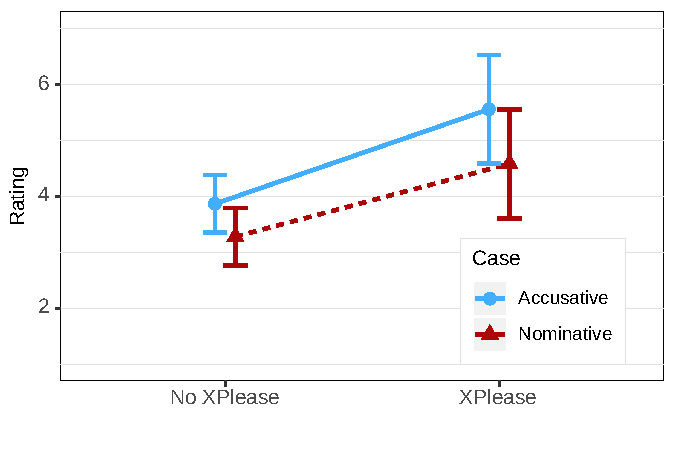
\includegraphics[width=10cm]{figures/ex1_case_estimates}
 \caption{Mean ratings and 95\% confidence intervals across conditions in experiment \ref{exp:case}. \label{fig:case-estimates}}
\end{figure}

I analyzed the data with CLMMs as described in Section \ref{sec:intro-stats}. The full model contained fixed effects for \textsc{Case} (binary), \textsc{XPlease} (binary) and the \textsc{Position} of the trial in the time-course of the experiment (numeric). The model included by-subject and by-item random intercepts and by-subject random slopes for \textsc{Case}, \textsc{XPlease} and their interaction. For items, I included only random slopes for \textsc{Case}, as \textsc{XPlease} was not varied systematically across token sets. The only fixed effects in the final model were those for \textsc{Case} and \textsc{XPlease} (see Table \ref{tab:case-estimates}): The main effect for \textsc{Case} shows that nominative\is{Nominative case} fragments were rated\is{Acceptability rating task} significantly as worse than accusative\is{Accusative case} fragments \clmmLR{7.39}{0.01}. The \textsc{XPlease} effect shows that fragments that could be paraphrased with an \textsc{XPlease} construction were significantly more acceptable than the others \clmmLR{7.3}{0.01}. There was no significant interaction between both predictors.

\begin{table}[t]
\begin{tabular}{l l l l l l}
\lsptoprule
Predictor & Estimate & SE & $\chi^2$ &  $p$-value &  \\   
\midrule
\textsc{Case} & -0.828 &  0.286 &7.39 & \textless 0.01 & ** \\
\textsc{XPlease} &    \phantom{-}1.875 &     0.632 &   7.30 &  \textless 0.01 & **\\
\lspbottomrule
\end{tabular}
\caption{Fixed effects in the final CLMM for experiment \ref{exp:case}. \label{tab:case-estimates}}
\end{table}

\subsubsection{Discussion}
Experiment \ref{exp:case} investigated case connectivity effects\is{Case connectivity} in German\is{German} accusative\is{Accusative case} DP\is{Determiner phrase} fragments, which would indicate unarticulated structure in fragments and hence provide evidence for a sentential theory of fragments. The data suggest that structural (accusative\is{Accusative case}) case marking is possible in fragments. Even in the absence of an explicit linguistic antecedent, accusative\is{Accusative case} DP\is{Determiner phrase}s are rated\is{Acceptability rating task} at least as acceptable as nominative\is{Nominative case} ones. In fact, the significant main effect of \textsc{Case} shows that accusative\is{Accusative case} is rated\is{Acceptability rating task} even better than nominative\is{Nominative case} if a full sentence requiring accusative\is{Accusative case} is accessible in context. This pattern is unexpected under the nonsentential account\is{Nonsentential account}, according to which accusative\is{Accusative case} is ungrammatical, but predicted by sentential accounts. From a sentential perspective, the acceptability of accusative\is{Accusative case} is analyzed as a case connectivity effect: Accusative case marking on the DP\is{Determiner phrase} is also required in the sentential alternative to the fragment, whose salience the pretest confirmed. If the data are to be explained by case connectivity\is{Case connectivity}, the lower ratings for nominative\is{Nominative case} indicate that a sentence that requires nominative\is{Nominative case} is unavailable, or at least less accessible in the case of my materials. 

This assumption has not been tested in the pretest, though. Even if the full sentence that requires accusative\is{Accusative case} was rated\is{Acceptability rating task} as perfectly natural in the pretest, this does not exclude the possibility that there is an equally accessible sentence that requires nominative\is{Nominative case}. In such a situation, the sentential account would predict no difference in acceptability between accusative\is{Accusative case} and nominative\is{Nominative case} fragments for my materials: No matter in which case the fragment appears, an antecedent for ellipsis resolution is accessible. If this was the case, the preference for accusative\is{Accusative case} in experiment \ref{exp:case} would still challenge the nonsentential account\is{Nonsentential account}, but neither would be in line with the case connectivity\is{Case connectivity} explanation that would provide evidence for sentential accounts of fragments. I address this issue with experiment \ref{exp:case-production}.

The \textsc{XPlease} predictor ensures that the overall preference for accusative\is{Accusative case} is not driven by only a few influential data points that might result from a conventionalized usage of accusative\is{Accusative case} fragments in contexts of ordering. In fact, the significant main effect of \textsc{XPlease} shows that these items are perceived as more acceptable than the remaining fragments. However, they were rated\is{Acceptability rating task} better in both \textsc{Case} conditions, and the absence of an interaction between \textsc{XPlease} and \textsc{Case} evidences that the preference for accusative\is{Accusative case} is independent of this construction. Possibly, in the potential \textsc{XPlease} construction the QuD\is{Question under Discussion} was easier to figure out or it is socially more appropriate to communicate with a fragment in such situations.

\largerpage
Table \ref{tab:ex-case-theories} summarizes different fragment theories' predictions on structural case-marking. If accusative\is{Accusative case} is structural case\is{Structural case} in German\is{German}, i.e. a purely linguistic device marking a structural relationship between the verb and its complement, the preference for accusative\is{Accusative case} clearly supports a sentential analysis. This holds even in the absence of explicit linguistic context\is{Context, linguistic}. Consequently, it is not an option to claim that short answers\is{Fragment, short answer} are elliptical and thus exhibit connectivity effects\is{Case connectivity}, while discourse-initial fragments\is{Fragment, discourse-initial} are genuine nonsententials and do not. %

\begin{table}[t]
\begin{tabular}{l l l }
\lsptoprule
 & Nominative\is{Nominative case} & Accusative\is{Accusative case} \\
\midrule
Nonsentential account\is{Nonsentential account} & \phantom{(}\ding{51}\phantom{)} & \ding{55}\\
Sentential account\is{In situ deletion account}\is{Movement and deletion account} & (\ding{51}) & \ding{51}\\
Ungrammatical\is{Ungrammaticality of fragments} & (\ding{51}) & \ding{51}\\
\hline
Experiment \ref{exp:case} & \phantom{(}\ding{55}\phantom{)} &\ding{51} \\
\lspbottomrule

\end{tabular}
\caption{Summary of the predictions of fragment theories on structural case marking. \label{tab:ex-case-theories}}
\end{table}

Of course, the conclusion that the data challenge the nonsentential account\is{Nonsentential account} relies strongly on the theoretical distinction between structural, default\is{Default case} and inherent\is{Inherent case} case assumed by \citet{barton.progovac2005}: If accusative\is{Accusative case} was analyzed as inherent\is{Inherent case} case, the data would not conflict with the nonsentential account\is{Nonsentential account}. However, in Section \ref{sec:theories-predictions-case} I showed that the diagnostics presented by \citet{progovac.etal2006} as evidence that the Serbian\is{Bosnian/Croatian/Serbian} accusative\is{Accusative case} is indeed inherent\is{Inherent case} case yield the opposite result for German\is{German}.

\noindent So far, the data are in line with \citepos{bergen.goodman2015} view that fragments are \textit{per se} ungrammatical but can be used as long as it is relatively easy to retrieve the omitted material. Any cue that guides the hearer toward the intended meaning will be useful for this purpose, and accusative\is{Accusative case} is definitely such a cue, because parsing the accusative\is{Accusative case} DP\is{Determiner phrase} rules out all possible meanings that require it to appear in a different case. Furthermore, as \citet{progovac.etal2006} note, accusative\is{Accusative case} DP\is{Determiner phrase}s will be relatively likely to be assigned the patient \texttheta-role. Furthermore, any case functions as a cue toward the associated \texttheta-role to some extent, as even the relatively unmarked nominative\is{Nominative case} reduces the likelihood of the DP\is{Determiner phrase} being a recipient (which usually receives dative\is{Dative case} case marking). However, this reasoning cannot reconcile the data with the nonsentential account\is{Nonsentential account} by \citet{barton.progovac2005}, who emphasize the categorical distinction between default\is{Default case}, inherent\is{Inherent case} and structural case.

\refstepcounter{expcounter}\label{exp:case-production}
\subsection{Experiment \ref{exp:case-production}: Default case, production study}
\label{sec:fragments-case-followup}
\subsubsection{Motivation}

Experiment \ref{exp:case-production} tested whether a sentential alternative that requires accusative\is{Accusative case} is indeed more salient in the context of the materials tested in experiment \ref{exp:case} than one that requires nominative\is{Nominative case}. Only in that case, the preference for accusative\is{Accusative case} in experiment \ref{exp:case} can be attributed to case connectivity\is{Case connectivity} and hence be interpreted as evidence for a sentential theory of fragments.

From a sentential perspective, the preference for accusative\is{Accusative case} in experiment \ref{exp:case} is explained by the availability of a linguistic antecedent for ellipsis which contains a verbal node licensing accusative\is{Accusative case} case marking on the fragment DP\is{Determiner phrase}. The salience of such an antecedent is confirmed by the high naturalness of sentential alternatives to the DP\is{Determiner phrase} fragments evidenced in the pretest. This line of reasoning, however, implies that a sentence that requires nominative\is{Nominative case} on the DP\is{Determiner phrase} is less accessible, because nominative\is{Nominative case} was perceived as less acceptable in experiment \ref{exp:case}. Since the pretest investigated only sentences containing accusative\is{Accusative case} DP\is{Determiner phrase}s, it is still possible that a sentence requiring nominative\is{Nominative case} is equally likely and the acceptability ratings\is{Acceptability rating task} call for a different explanation. Experiment \ref{exp:case-production} addresses this issue with a production study\is{Production task} using the same materials as experiment \ref{exp:case}. In contrast to the rating study, subjects produced the target utterance themselves. I then quantified the preference for full sentences that required accusative\is{Accusative case} or nominative\is{Nominative case} case marking on the fragment based on the aggregated responses.

\subsubsection{Materials}
The context stories of experiment \ref{exp:case} were used as stimuli in a production task\is{Production task}. Instead of reading a fragment, as in experiment \ref{exp:case}, subjects saw a hand-drawn image of the object referred to by the DP\is{Determiner phrase} fragment (see Figure \ref{fig:production-stim}%
\footnote{\copyright Julia Stark. This image is released under a CC-BY license.}\afterfn%
%
for an example). Subjects were asked to read the story and to produce an utterance by the specified character that referred to the depicted object. The use of graphical stimuli avoided the problem that some (but not all) of the nouns in the DP\is{Determiner phrase} fragments tested in experiment \ref{exp:case} morphologically distinguish accusative\is{Accusative case} and nominative\is{Nominative case}, so that a written presentation would have introduced a case bias.

\begin{figure}[t]
 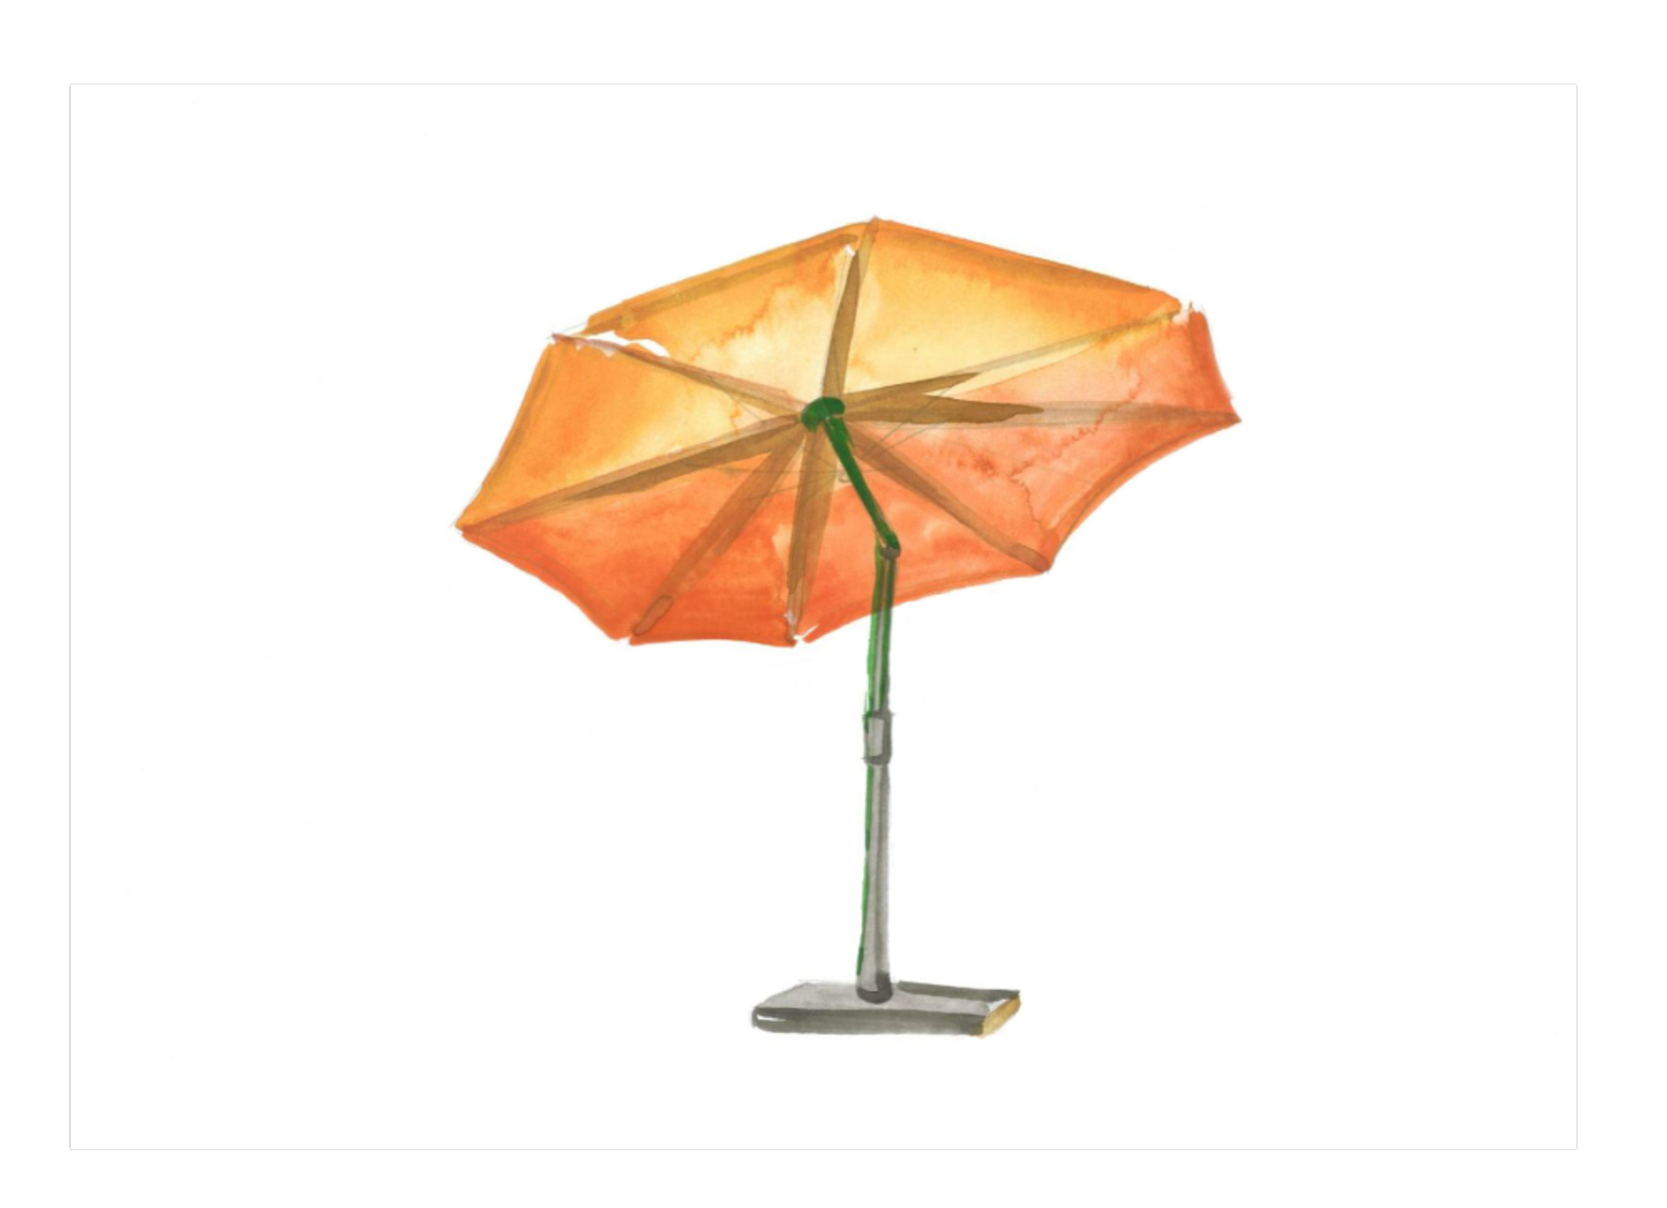
\includegraphics[scale=.3]{figures/production_sunshade.pdf}
 \caption{Sample graphical stimulus used in experiment \ref{exp:case-production}.\label{fig:production-stim}}
\end{figure}

\subsubsection{Procedure}
The experiment was conducted over the Internet using the LimeSurvey survey presentation software and completed by 38 undergraduate students of Saarland University. They were rewarded with the participation in a lottery of 5 $\times$ \currencyEuro{30} among all participants. Subjects read the context story, which was presented above a hand-drawn image that depicted the object referred to by the corresponding DP\is{Determiner phrase} fragment in experiment \ref{exp:case}. They were asked to enter an utterance that was likely to be said by a specified character and that referred to the depicted object into a text field. As there was only one condition, all subjects saw the same materials. The experiment was presented to the same subjects as the acceptability rating\is{Acceptability rating task} study for \ref{exp:mvb} and the follow-up to experiment \ref{exp:ccs-german}. As the context stories contained no specifically biasing patterns that might prime subjects, there were no fillers, so that each subject produced 20 responses. The stimuli were presented in individually fully randomized order. The responses were manually annotated for the \textsc{Case} of the DP\is{Determiner phrase} referring to the image and the noun used in the DP\is{Determiner phrase} by the subjects. It was also annotated whether the subjects used the same lemma as tested in experiment \ref{exp:case}, a synonym, or whether they did not mention the lemma or a synonym at all. Responses that did not refer to the object depicted by the image (14.96\% of the data) were excluded from further analysis.

\subsubsection{Results}
There was a strong overall preference for accusative\is{Accusative case} (88.78\% of all trials) over nominative\is{Nominative case} (5.03\% of trials). The remaining 6.19\% of trials used other constructions that contained a DP\is{Determiner phrase} in dative\is{Dative case} or prepositional case\is{Prepositional case}.%
%
\footnote{In this context, prepositional case\is{Prepositional case} was always dative\is{Dative case} or accusative\is{Accusative case}. I distinguish prepositional case\is{Prepositional case} from other uses of dative\is{Dative case} and accusative\is{Accusative case} because e.g. \citet{zwarts2005} shows that prepositional case\is{Prepositional case} is in part determined by the preposition and not related to structure (accusative\is{Accusative case}) or a \texttheta-role (dative\is{Dative case}).}\afterfn%
%
The noun lemma produced by the subjects was the same as tested in experiment \ref{exp:case} in 49.7\% of the trials, a synonymous one in another 38.4\% and a closely related one (e.g. \textit{salad} instead of \textit{pasta salad}) in 11.9\% of the trials.

\begin{table}[t]
\begin{tabular}{l l l l l l}
\lsptoprule
Predictor & Estimate & SE & $\chi^2$ &  $p$-value &  \\   
\midrule
Intercept & -2.657 & 0.245 & 37.58 & \textless \highsig & *** \\
\lspbottomrule
\end{tabular}
\caption{Fixed effects in the final GLM for experiment \ref{exp:case-production}. \label{tab:case-production-estimates}}
\end{table}

Since the purpose of the experiment was to investigate the relative likelihood of accusative\is{Accusative case} and nominative\is{Nominative case} when referring to the target DP\is{Determiner phrase} and there were no predictors, I analyzed the data with an intercept-only logistic regression conducted with the \texttt{lme4} \citep{bates.etal2015} package in \texttt{R} \citep{rcoreteam2019}. The intercept of such a model indicates the likelihood of an observation to fall into one of the two categories, so that a significant intercept will show that these categories are not equally likely. The model in Table \ref{tab:case-production-estimates} shows that this is the case \glmer{37.58}{\highsig}. 

\subsubsection{Discussion}
Experiment \ref{exp:case-production} investigated whether a full sentence that requires accusative\is{Accusative case} case marking on the DP\is{Determiner phrase} fragment is indeed more likely than a sentence requiring nominative\is{Nominative case}. If this was the case, the pattern found in experiment \ref{exp:case} would indicate case connectivity\is{Case connectivity} and support a sentential theory of fragments. The production study\is{Production task} shows that accusative\is{Accusative case} was used significantly more often than nominative\is{Nominative case} in order to name the object referred to by the DP\is{Determiner phrase} fragment in experiment \ref{exp:case}. This is expected if the preference for accusative\is{Accusative case} or nominative\is{Nominative case} in experiment \ref{exp:case} is due to case connectivity\is{Case connectivity}: Accusative is preferred, because a full sentence that requires accusative\is{Accusative case} is the most salient antecedent for ellipsis that is made available through the context story. Taken together, experiments \ref{exp:case} and \ref{exp:case-production} provide clear evidence for unarticulated structure in fragments. First, fragments \textit{can} exhibit structural case morphology, and second, they \textit{do so} preferably when a fully sentential structure requiring structural case is salient in context.

\refstepcounter{expcounter}\label{exp:scripts-rating-case}
\subsection{Experiment \ref{exp:scripts-rating-case}: Mixed accounts?}  \label{sec:scripts-rating-case}
\subsubsection{Background}
\is{Mixed account|(}

Experiments \ref{exp:case} and \ref{exp:case-production} show that in contexts where a DP\is{Determiner phrase} appears in accusative\is{Accusative case} (structural case) in full sentences in German\is{German}, accusative\is{Accusative case} DP\is{Determiner phrase} fragments are also preferred over nominative\is{Nominative case} (default case\is{Default case}) DP\is{Determiner phrase} fragments. This finding is unexpected under the nonsentential account\is{Nonsentential account} by \citet{barton.progovac2005}, but it indicates case connectivity effects\is{Case connectivity}, which sentential accounts predict.

This result does not imply that \textit{all} fragments are generated by ellipsis. \citet{barton2006} raises the possibility of a \textit{mixed} account\is{Mixed account} of fragments, which derives some fragments  by ellipsis, whereas others are genuine nonsententials. Such an account would be motivated by the observation that the properties of fragments cannot be captured by a single syntactic mechanism alone. For instance, there might be both instances of case connectivity\is{Case connectivity} and anticonnectivity\is{Case connectivity}, so that both the nonsentential\is{Nonsentential account} and a sentential derivation would have to be assumed.

From a theoretical perspective, even that a mixed account\is{Mixed account} might account for the relevant data, Occam's Razor requires us to adopt one of the simpler accounts, unless a mixed captures the empirical picture better. To my knowledge, few serious attempts have been made to work out a mixed account\is{Mixed account} of fragments in detail. \citet{barton2006} cites \citet{morgan1989} and herself \citep{barton1998} as mixed account\is{Mixed account}s, but notes considerable differences between both with respect to the scope attributed to the sentential and nonsentential\is{Nonsentential account} generation mechanisms\is{Nonsentential account}. According to \citet{barton2006}, \citeauthor{morgan1989} adopts the nonsentential analysis\is{Nonsentential account} only for fragments that (arguably) cannot be explained by the sentential accounts, such as case-less Korean \is{Korean} DPs\is{Determiner phrase}, whereas \citet{barton1998} analyzes only those fragments that cannot be derived as genuine nonsententials as elliptical sentences. 

No matter how many of the empirically observed fragments are attributed to either derivation mechanism, spelling out a mixed account\is{Mixed account} necessarily involves explaining why the (non)sentential derivation is (not) available or (dis)\-preferred in a specific context. A straightforward implementation of a mixed account\is{Mixed account} could assume that a trade-off between the effort\is{Processing effort} required to find an antecedent that licenses ellipsis and a cost for pragmatic enrichment \citep{sperber.wilson1986, sperber.wilson1995,breheny.etal2006,  chevallier.etal2008} determines whether ellipsis resolution or pragmatic enrichment is used in order to interpret a fragment.%
%
\footnote{This is obviously the perspective of the hearer. However, since I assume that the speaker performs audience design\is{Audience design} \citep{bell1984}, the speaker will adapt her utterance to expectations about the interpretive behavior of the hearer.}\afterfn%
%
If pragmatic inference is effortful\is{Processing effort}, syntactic ellipsis resolution will be preferred when it is easy to retrieve an antecedent. The more difficult this retrieval becomes, the more promising might be the nonsentential derivation\is{Nonsentential account} that requires pragmatic inference by the hearer. A mixed account\is{Mixed account} based on this idea predicts case connectivity\is{Case connectivity} if there is a salient antecedent for ellipsis resolution and the generation of genuine nonsententials in case no salient antecedent is available.%
%
\footnote{The mixed account\is{Mixed account} would obviously have to explain why a fragment is used at all if there is no salient antecedent that guides toward the meaning intended by the speaker.}\afterfn%
%

In experiment \ref{exp:case} I investigated only fragments that have a salient antecedent. Since the mixed account\is{Mixed account} predicts that such fragments are better resolved by ellipsis, it agrees with the sentential account in this case. However, if no salient antecedent is available, the mixed account\is{Mixed account} predicts that fragments are generated as nonsententials\is{Nonsentential account}. If genuine nonsentential utterances do not exhibit case connectivity\is{Case connectivity}, the predictions of sentential and nonsentential accounts diverge here: Sentential accounts predict strict case connectivity\is{Case connectivity}, and under the mixed account\is{Mixed account} sketched above structural case should be unavailable.

\begin{table}[t]
\begin{tabular}{l c c c c}
\lsptoprule
 & \multicolumn{2}{c}{Predictable} & \multicolumn{2}{c}{Unpredictable} \\
 & Nom. & Acc.& Nom. & Acc.\\
\midrule
Nonsentential account &\ding{51} & \ding{55} & \ding{51} & \ding{55}\\
Sentential account & (\ding{51}) & \ding{51} & (\ding{51}) & \ding{51}\\
Mixed account & (\ding{51}) &\ding{51} & \ding{51} & \ding{55} \\
\lspbottomrule
\end{tabular}
 
\caption{Summary of the predictions of the nonsentential, sentential and mixed account with respect to experiment \ref{exp:scripts-rating-case}. \label{tab:scripts-case-theories}}
\end{table}

In experiment \ref{exp:scripts-rating-case} I therefore compared the acceptability\is{Acceptability rating task} of accusative\is{Accusative case} and nominative\is{Nominative case} fragments in predictable and unpredictable contexts in a 2$\times$2 design crossing \textsc{Predictability} and \textsc{Case} in an acceptability rating study\is{Acceptability rating task}. The predictions of the sentential, nonsentential\is{Nonsentential account} and mixed account\is{Mixed account} are summarized in Table \ref{tab:scripts-case-theories}. The nonsentential accounts\is{Nonsentential account} again predicts that accusative\is{Accusative case} is ungrammatical and that nominative\is{Nominative case} default case\is{Default case} is preferred. The sentential account predicts case connectivity\is{Case connectivity}: If there is a salient full sentence that requires accusative\is{Accusative case}, accusative\is{Accusative case} will be preferred. Finally, the mixed account\is{Mixed account} matches the behavior of the nonsentential account\is{Nonsentential account} for unpredictable fragments and that of the sentential account for predictable fragments. Fragments can be generated by ellipsis in predictive contexts, but are genuine nonsententials if no salient antecedent is available. 

\is{Mixed account|)}

\subsubsection{Materials}
The materials were derived from those used in experiment \ref{exp:scripts-rating} (see Section \ref{sec:scripts-rating}).The predictability of fragments was manipulated with context stories\is{Context, extralinguistic} based on event chains\is{Event chain} derived from the DeScript \citep{wanzare.etal2016} corpus\is{Corpus} of script knowledge\is{Script knowledge}.%
%
\footnote{In experiment \ref{exp:scripts-rating} some DPs\is{Determiner phrase} were ambiguous between accusative\is{Accusative case} and nominative\is{Nominative case} case. I replaced these DPs\is{Determiner phrase} by a semantically similar masculine singular noun that distinguishes accusative\is{Accusative case} and nominative\is{Nominative case} or chose a different event sequence from the same script.}\afterfn%
%
This ensures that the \textsc{Predictability} manipulation is founded on empirically observed event probabilities. In very simplified terms, the corpus\is{Corpus} allows for the estimation of the likelihood of an event in a script-based scenario given the previous events. For instance, a person who is cooking pasta will be likely to pour the pasta into the pot after the water is boiling. Under the assumption that likely events are more likely to be talked about than unlikely ones,%
%
\footnote{See Sections \ref{sec:scripts-rating-discussion} and \ref{sec:scripts-production-background} for a discussion.}\afterfn%
%
the likelihood of utterances in context can be quantified and manipulated based on the corpus\is{Corpus} data (see Section \ref{sec:infotheory-script-event-chains} for details). The stimuli consisted of short context stories of three sentences each and a fragment uttered by one of the characters introduced in the story \Next. The fragments were DPs\is{Determiner phrase} that referred to an event that was either predictable \Next[a,b] or unpredictable \Next[c,d] given the corpus\is{Corpus} data. 

\ex. Today, Marie and Jonas want to cook themselves a large serving of pasta with tomato sauce. As soon as the water started to boil, Jonas has added the pasta. After ten minutes, he says to Marie:
\ag. Der Topf mit den Nudeln.\\
     the.\textsc{nom} pot with the.\textsc{acc} pasta\\ 
     \exsourcefrombelow{Predictable, nominative}
\bg. Den Topf mit den Nudeln.\\
     the.\textsc{acc} pot with the.\textsc{acc} pasta\\
     \trans{The pot with the pasta.}  \exsourceraised{Predictable, accusative}
\cg. Der Küchentisch.\\
     the.\textsc{nom} kitchen.table\\ \exsourcefrombelow{Unpredictable, nominative}
\dg. Den Küchentisch.\\
     the.\textsc{acc} kitchen.table\\
     \trans{The kitchen table.} \exsourceraised{Unpredictable, accusative}

In both cases, in the corresponding full sentence \Next with default word order\is{Word order} the fragment appears in a post-verbal position and exhibits accusative\is{Accusative case} case morphology. In the predictable condition, the underlying sentence \Next[a] refers to the most likely event to follow the sequence of events underlying the context story, which is \textit{remove the pot from the stove} in the example. The context story refers to the events\is{Event chain} \textit{water starts to boil}, \textit{add pasta to the water} and \textit{cook pasta}. In the unpredictable condition, the event that the target utterance \Next[b] referred to (\textit{set table}) was not mentioned in the corpus\is{Corpus} data, but it is intuitively not fully implausible.     
     
\ex. \ag. Nimm  den Topf mit den Nudeln vom Herd.\\
	  take.\textsc{imp} the.\textsc{acc} pot with the.\textsc{acc} pasta off-the.\textsc{dat} stove\\
	  \trans{Take the pot with the pasta off the stove.}
     \bg. Deck doch schonmal den Küchentisch.\\
	  set.\textsc{imp} \textsc{prt} already the.\textsc{acc} kitchen.table\\
	  \trans{Set the kitchen table, please.}

In principle, it would have been desirable to keep the target utterance as constant as possible across conditions and to vary only those properties that are related to the variables that are investigated by presenting a single fragment in an unpredictive and a predictive context. However, if an unpredictive context for the fragment in \LLast[a] that is not based on the corpus\is{Corpus} data had been constructed from scratch, it would have been impossible to quantify the likelihood of the \textit{remove pot} event in the same fashion as in the predictable condition. This likelihood could also be measured in a norming study, but this would have required considerably more effort than relying on the corpus\is{Corpus}-based probabilities that were available from experiment \ref{exp:scripts-rating}. Alternatively, the fragment could have been presented with a different corpus\is{Corpus}-based context story for which it is known that the corresponding event does not happen (e.g. describing the train ride scenario) in the unpredictable condition. In this case though, the target utterance would not only be unlikely, but actually implausible and therefore probably highly degraded in any \textsc{Case} condition.

\subsubsection{Procedure}
The experiment, which was conducted on the Internet via LimeSurvey, was completed by 47 native speakers of German\is{German}, who were recruited through the crowdsourcing platform \textit{clickworker}. Subjects were paid \currencyEuro{4} for participating in the study. They were asked to rate the naturalness of the italicized target utterance in the context of the story on a 7-point Likert scale (7 = fully natural). Subjects were randomly assigned to one of four lists, to which the materials were distributed according to a 2$\times$2 Latin square design. Each subject saw each token set once and only in one condition. Each subject rated\is{Acceptability rating task} 24 items (six per condition), which were mixed with 16 items from an unrelated experiment and 44 fillers. Materials were presented in a pseudorandomized order that ensured that no two items of the same experiment followed each other. Fillers consisted of context stories followed by an utterance by one of the characters or a question-answer pair. In the latter case, subjects rated\is{Acceptability rating task} the answer, which was presented in italicized font. Six fillers with ungrammatical word order\is{Word order} served as attention checks. Three subjects who rated\is{Acceptability rating task} 50\% or more of the attention checks as acceptable (6 or 7 points on the scale) were excluded from further analysis.

\begin{figure}[t]
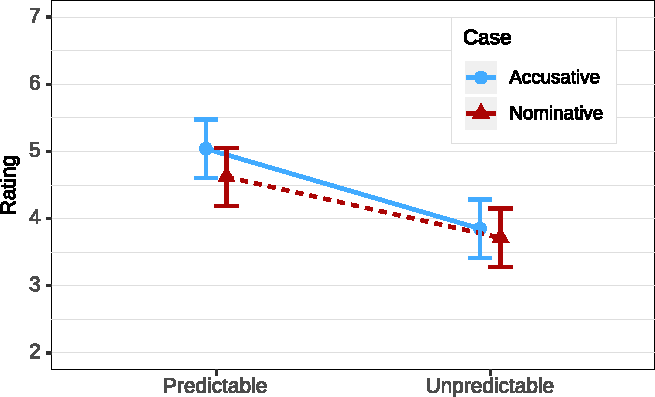
\includegraphics[scale=1]{figures/scripts_case_estimates}
\caption{Mean ratings and 95\% confidence intervals across conditions in experiment \ref{exp:scripts-rating-case}. \label{fig:scr-case-estimates}}
\end{figure}

\subsubsection{Results}
Figure \ref{fig:scr-case-estimates} shows the averaged ratings across conditions. The data were analyzed with CLMMs following the procedure described in Section \ref{sec:intro-stats}. The full model contained main effects for \textsc{Case}, \textsc{Predictability} and the \textsc{Position} of the item in the time-course of the experiment, as well as by-subject and by-item random intercepts and slopes for \textsc{Case}, \textsc{Predictability} and their interaction. Random effects of \textsc{Position} and its interaction with the other predictors were removed because models did not converge otherwise. The final model (see Table \ref{tab:scripts-case-estimates}) contained only a significant main effect for \textsc{Predictability} \clmmLR{10.04}{0.01}. Neither the main effect of \textsc{Case} \clmmLRnonsig{2.5}{0.1} nor its interaction with \textsc{Predictability} \clmmLRnonsig{1.78}{0.1} were significant.

\begin{table}[t]
\begin{tabular}{l l l l l l}
\lsptoprule
Predictor & Estimate & SE & $\chi^2$ &  $p$-value &  \\   
\midrule
\textsc{Predictability} & -1.25 &  0.35 & 10.04 & \textless 0.01 & ** \\
\lspbottomrule
\end{tabular}
\caption{Fixed effects in the final CLMM for experiment \ref{exp:scripts-rating-case}. \label{tab:scripts-case-estimates}}
\end{table}

\subsubsection{Discussion}
The purpose of experiment \ref{exp:scripts-rating-case} was to test a mixed account\is{Mixed account} of fragments. Mixed accounts assume that speakers use two different mechanisms to interpret (and produce) fragments, which differ in their predictions with respect to case marking: If fragments are generated by ellipsis from full sentences, they can exhibit structural case marking\is{Case connectivity}, but if they are base-generated as genuine nonsententials\is{Nonsentential account}, they cannot. It is a natural assumption that speakers resort to ellipsis when there is a salient antecedent that allows resolution and to pragmatic inference when there is no such antecedent. Consequently, the mixed account\is{Mixed account} predicts that nominative\is{Nominative case} is rated\is{Acceptability rating task} as better than accusative\is{Accusative case} in the unpredictable condition, where it is more difficult to retrieve an antecedent for ellipsis. The absence of a significant interaction between \textsc{Case} and \textsc{Predictability} shows that this prediction is not borne out. Unpredictable fragments are significantly worse than predictable fragments, but this holds independently of case.

In contrast to experiment \ref{exp:case}, there was no significant main effect of \textsc{Case}. This might be due to a reduced accessibility of antecedents that require nominative\is{Nominative case} in the materials for experiment \ref{exp:scripts-rating-case} as compared to those used in experiment \ref{exp:case}. Whether this is correct could be tested with a further production study\is{Production task}. However, this goes beyond the scope of this experiment, which was designed to test whether nominative\is{Nominative case} is relatively more acceptable in unpredictable fragments.

Taken together, experiment \ref{exp:scripts-rating-case} provides further evidence against the nonsentential account\is{Nonsentential account}. Unlike what the nonsentential account\is{Nonsentential account} predicts, fragments are not rated\is{Acceptability rating task} better in nominative\is{Nominative case} than in accusative\is{Accusative case}. The pattern observed in experiment \ref{exp:scripts-rating-case} is unexpected both under the nonsentential\is{Nonsentential account} and the mixed account\is{Mixed account}.

\subsection{General discussion: Structural case marking}
I presented three experiments that investigated whether fragments are derived from regular sentences by ellipsis or whether they are genuine nonsententials\is{Nonsentential account}. The experiments used structural case marking on discourse-initial\is{Fragment, discourse-initial} DP\is{Determiner phrase} fragments as a diagnostic for unarticulated structure. In minimalism\is{Minimalist program}, the framework that underlies both the nonsentential and most of the sentential accounts discussed in Chapter \ref{sec:chapter-theories}, structural case\is{Structural case} must be checked\is{Case feature} by a verbal head. If, as nonsententialists argue, there is no unarticulated structure in fragments, structural case marking must be unavailable in fragments. In contrast, according to sentential accounts there is an unarticulated verbal head in DP\is{Determiner phrase} fragments, so that they are expected to appear in structural case\is{Structural case} whenever they do in the corresponding full sentence\is{Case connectivity}. Experiments \ref{exp:case}--\ref{exp:scripts-rating-case} investigated this using the example of German\is{German}, where accusative\is{Accusative case} is a structural case and nominative\is{Nominative case} the default case\is{Default case}, if such a concept is to be assumed at all. Experiment \ref{exp:case} showed that if there is a salient antecedent that licenses accusative\is{Accusative case}, DP\is{Determiner phrase} fragments can appear in accusative\is{Accusative case} case. In fact, accusative\is{Accusative case} was rated\is{Acceptability rating task} even better than nominative\is{Nominative case}. This disconfirms the prediction of the nonsentential account\is{Nonsentential account} and in turn supports sentential accounts. Experiment \ref{exp:case-production} showed that in the context of my materials a full sentence requiring accusative\is{Accusative case} on the DP\is{Determiner phrase} was indeed more likely than one requiring nominative\is{Nominative case}. This finding further strengthens the interpretation of experiment \ref{exp:case} as evidence for connectivity effects\is{Case connectivity}. Finally, experiment \ref{exp:scripts-rating-case} explored the predictions of a mixed account\is{Mixed account} that assumes that fragment generation by ellipsis is possible, but restricted to contexts where an antecedent is available. Therefore, I tested whether nominative\is{Nominative case} is more acceptable when the corresponding sentence is relatively unpredictable. Since there was no such effect, the data speak against the mixed account\is{Mixed account} that I sketched.

It must be emphasized that this interpretation of the data presupposes that the categorical difference between structural and inherent\is{Inherent case} case assumed by \citet{barton.progovac2005} is correct. This distinction is crucial to the nonsentential account\is{Nonsentential account}, since \citet{barton.progovac2005} rely on it to explain crosslinguistic differences between English\is{English} and Serbian\is{Bosnian/Croatian/Serbian} as well as acceptability contrasts within English\is{English}. Nonsentential accounts that do not rely on the inherent\is{Inherent case}/structural case distinction as heavily as \citet{barton.progovac2005} do, like analyses in the simpler syntax framework\is{Simpler syntax} \citep{culicover.jackendoff2005} or in HPSG\is{HPSG} \citep{ginzburg.sag2000, fernandez.ginzburg2002} might still be able to explain the data. The data are also in line with the idea that fragments are ungrammatical, but can point toward the meaning intended by a speaker, as suggested by \citet{bergen.goodman2015}\is{Ungrammaticality of fragments}. Since accusative\is{Accusative case} case in fragments might indicate that the DP\is{Determiner phrase} fragment is to be interpreted as patient or object, a preference for accusative\is{Accusative case} is expected under this account, if the DP\is{Determiner phrase} fragment is the object of a transitive verb in a corresponding complete sentence. 

Furthermore, the predictions of the nonsentential account\is{Nonsentential account} also rely on the classification of a particular case as structural or inherent\is{Inherent case}. \citet{barton.progovac2005} argue that nominative\is{Nominative case} is structural case in English\is{English}, but default case\is{Default case} in Serbian\is{Bosnian/Croatian/Serbian}, so that nominative\is{Nominative case} DP\is{Determiner phrase} fragments are predicted to be ungrammatical in English\is{English}, but not in Serbian\is{Bosnian/Croatian/Serbian}. The conclusions that I draw from my data rely on the assumption that accusative\is{Accusative case} is indeed structural case in German\is{German}. \citet{progovac.etal2006} argued that accusative\is{Accusative case} is inherent\is{Inherent case}, semantically interpretable, case in German\is{German}, and if this is correct, the nonsentential account\is{Nonsentential account} would correctly predict German\is{German} accusative\is{Accusative case} DP\is{Determiner phrase} fragments to be acceptable. I argued above that, given the tests used by \citet{progovac.etal2006} for Serbian\is{Bosnian/Croatian/Serbian}, accusative\is{Accusative case} must be classified as structural case in German\is{German}, so that the nonsentential account\is{Nonsentential account} makes incorrect predictions. 

Even though the experiments did not explicitly test the predictions of a con\-struc\-tion-\is{Construction grammar}based account, they suggest that the acceptability of accusative\is{Accusative case} case cannot be explained by the assumption of a conventionalized construction like e.g. $\langle$DP\is{Determiner phrase}$\rangle$\textsubscript{Acc}: Both in experiments \ref{exp:case} and \ref{exp:scripts-rating-case}, the acceptability of accusative\is{Accusative case} does not vary as a function of the predictability or degree of conventionalization of the fragment. Of course this does not rule out the possibility that some fragments are stored as constructions in the mental lexicon, but this cannot explain the acceptability of accusative\is{Accusative case} DP\is{Determiner phrase} fragments in my experiments.

\noindent Taken together, the experiments presented in this section support a sentential analysis of fragments against the nonsentential account\is{Nonsentential account} by \citet{barton.progovac2005}. They furthermore empirically confirm two properties of fragments that have to be taken into account in the investigation of fragment usage: Fragments exhibit case connectivity\is{Case connectivity} and that they can appear in structural case\is{Structural case}.

Having established that fragments are underlyingly sentential, this leads to my second main research question on the syntax of fragments, that is, whether the generation of fragments involves movement to the left periphery \citep{merchant2004}\is{Movement and deletion account} or whether fragments result from \textit{in situ} deletion \citep{reich2007}\is{In situ deletion account}.

\newpage
\section{Movement restrictions: Preposition omission}
\label{sec:pstranding}

The experiments in Section \ref{sec:experiments-case} provided evidence for unarticulated syntactic structure in fragments, in particular for a silent verbal head that checks accusative\is{Accusative case} structural case\is{Structural case} in DP fragments. In the remainder of this chapter I investigate which kind of structure underlies fragments. The main controversy with respect to this question is whether the derivation of fragments involves obligatory movement to the left periphery. In Sections \ref{sec:theories-sentential} and \ref{sec:theories-predictions-movement} I outlined the positions: On the one hand, there is \citepos{merchant2004} influential movement and deletion\is{Movement and deletion account} account, which has been more recently adopted and partially modified by other researchers \citep[see e.g.][]{aelbrecht2009, sato2011,weir2014, doring2016, saab.liptak2016,  murphy2018} and assumes that the derivation of fragments involves obligatory movement to the left periphery. On the other hand, \textit{in situ} deletion\is{In situ deletion account} accounts \citep{reich2007, ott.struckmeier2016, griffiths.etal2018} derive fragments from regular sentences without assuming this obligatory movement step.

Since the \textit{in situ} deletion\is{In situ deletion account} approach does not require an additional movement operation in fragments, it is derivationally simpler. Therefore, the movement and deletion account\is{Movement and deletion account} requires additional evidence for movement in fragments. Such evidence consists in effects of movement restrictions\is{Movement restriction} on the form of fragments, which are then taken to indicate that left dislocation is a necessary step in the generation of fragments. \citet{merchant2004} discusses a series of such similarities between fragments and dislocation constructions, but even the brief discussion in Section \ref{sec:theories-predictions-movement} showed that not all of these parallelisms constitute genuine evidence for movement, because some of them can be explained under a non-movement account as well. Since the \textit{in situ} deletion\is{In situ deletion account} account is derivationally less complex than movement and deletion\is{Movement and deletion account}, I assume that it is the null hypothesis.%
%
\footnote{Actually the nonsentential account\is{Nonsentential account} is even simpler, but I rejected it in the preceding section because it does not capture the empirical picture correctly.}\afterfn%
%
Consequently, the movement and deletion\is{Movement and deletion account} account is only superior to \textit{in situ} deletion\is{In situ deletion account} if there are parallelisms between fragments and left dislocation that cannot be explained by the \textit{in situ} deletion\is{In situ deletion account} account. In my experiments I focus on three movement restrictions\is{Movement restriction} that have been claimed to or that might constrain the form of fragments. This section investigates restrictions on preposition stranding\is{Preposition stranding} and omission\is{Preposition omission} in German\is{German}, in Section \ref{sec:ccs} I address complement clause\is{Complement clause} topicalization and in Section \ref{sec:mvb} multiple prefield\is{Prefield} constituents in German\is{German}.

\subsection{Preposition omission as evidence for movement}\label{sec:pstranding-background}

\is{P-Stranding Generalization|(}
\subsubsection{The P-Stranding Generalization}\label{sec:pstranding-background-psg}
Among the movement restrictions\is{Movement restriction} that \citet{merchant2004} presents as evidence for his theory, the most compelling one is his \textit{P-Stranding Generalization}\is{P-Stranding Generalization} (PSG, in what follows). In a nutshell, the PSG\is{P-Stranding Generalization} states that only in those languages that allow for P-stranding\is{Preposition stranding} under regular \textit{wh}-movement it is possible to omit prepositions\is{Preposition omission} under sluicing\is{Sluicing} and in fragments. \citeauthor{merchant2004} takes this as evidence that P-stranding is a necessary step in the derivation of preposition-less answers\is{Fragment, short answer} to questions where the \textit{wh}-phrase corresponding to the answer is embedded within a PP\is{Preposition phrase}. English\is{English} is a typical example of a P-stranding language \Next. 

\ex. Who was Peter talking with?\hfill\citep[685]{merchant2004}\\
Mary.

Originally, \citet{merchant2001} introduced the PSG\is{P-Stranding Generalization} as evidence for his movement and deletion\is{Movement and deletion account} account of sluicing\is{Sluicing}. He presents introspective data from a relatively large and typologically diverse sample of languages%
%
\footnote{The data are from Arabic\is{Arabic}, Basque\is{Basque}, Czech\is{Czech}, Danish\is{Danish}, English\is{English}, Frisian\is{Frisian}, German\is{German}, Greek\is{Greek}, Hebrew\is{Hebrew}, Icelandic\is{Icelandic}, Irish\is{Irish}, Norwegian\is{Norwegian}, Polish\is{Polish}, Russian\is{Russian},  Serbo\is{Bosnian/Croatian/Serbian}-Croatian, Slovene\is{Slovene}, Swedish\is{Swedish} and Yiddish\is{Yiddish}.}\afterfn%
%
that overall show the predicted pattern. The contrast between languages that allow for P-stranding\is{Preposition stranding} and those with obligatorily pied-piping\is{Pied-piping} is exemplified in \Next and \NNext for English\is{English} and German\is{German}, respectively: English\is{English} allows for P-stranding\is{Preposition stranding} in \textit{wh}-questions \Next[a] and preposition omission\is{Preposition omission} under sluicing\is{Sluicing} \Next[b], whereas in German\is{German} the preposition is always pied-piped\is{Pied-piping} in \textit{wh}-questions \NNext[a] and realized in sluices\is{Sluicing} \NNext[b].

\ex.
\a. Who was he talking with? \label{pst-english-question}\hfill \citep[666]{merchant2004}
\b. Peter was talking with someone, but I don’t know (with) who.

\ex. 
\ag. *Wem hat sie mit gesprochen?\label{ex:pst-german-q}\\
Who.\textsc{dat} has she with talked\\
\trans{With whom was she talking?}\exsourceraised{\citep[667]{merchant2004}}
\bg. Anna hat mit jemandem gesprochen, aber ich wei\ss {} nicht, *(mit) wem. \hfill\\
Anna has with somebody.\textsc{dat} spoken but I know not \mbox{~~}with who.\textsc{dat}\\
\trans{Anna was talking with somebody, but I don't know (with) who.}

\newpage
\noindent The reasoning behind the PSG\is{P-Stranding Generalization} is that, if sluicing\is{Sluicing} is generated by regular \textit{wh}-movement as discussed above, the preposition cannot be omitted\is{Preposition omission} in German\is{German}, because this would require P-stranding\is{Preposition stranding} to occur during the derivation \Next. As P-stranding\is{Preposition stranding} is available in English\is{English} \LLast[a], but not in German\is{German} \Last[a], the corresponding sluice \LLast[b]/\Last[b] is grammatical in English\is{English}, but not in German\is{German}.%
%
\footnote{In German\is{German}, there are a few constructions which are similar to P-stranding\is{Preposition stranding}. In \Next, the particle \textit{her} contained in the complex \textit{wh}-phrase \textit{woher} can be stranded\is{Preposition stranding}, but in contrast to the PPs\is{Preposition phrase} providing evidence for the PSG\is{P-Stranding Generalization}, the moved element appears to the left of \textit{her} if no extraction occurs. See e.g. \citet{vanriemsdijk1978} for an analysis of such extractions in Dutch\is{Dutch}.

\ex. \ag. Wo hast du das Buch denn her?\\
	  where have you the book PART \textit{her}\\ 
\bg. Woher hast du das Buch denn?\\
	  where.from have you the book PART \textit{her}\\ 
	  \trans{Where did you get the book from?}

}\afterfn%
%

\ex. Peter was talking with someone, but I don't know who\textsubscript{i} \sout{Peter was talking with \textit{t}\textsubscript{i}}.

In his \citeyear{merchant2004} article, \citeauthor{merchant2004} extends this analysis to fragments\is{Fragment, short answer}. He argues that only languages that have P-stranding\is{Preposition stranding} allow for the omission of the preposition\is{Preposition omission} in short answers to questions whose \textit{wh}-phrase is the complement of a preposition. Again, the observation is supported by crosslinguistic data.%
% 
\footnote{The data are from Bulgarian\is{Bulgarian}, Czech\is{Czech}, Danish\is{Danish}, English\is{English}, German\is{German}, Greek\is{Greek}, Hebrew\is{Hebrew}, Icelandic\is{Icelandic}, Norwegian\is{Norwegian}, Russian\is{Russian}, Swedish\is{Swedish} and Yiddish\is{Yiddish} \citep[685--687]{merchant2004}.}\afterfn%
%
The contrast is exemplified here for English\is{English} \Next and German\is{German} \NNext.

\ex. 
Who was Peter talking with? \hfill\citep[685]{merchant2004} \label{ex:pstranding-fragments-english}\\
(With) Mary.

\exg. Mit wem hat Anna gesprochen?\\
with whom has Anna spoken?\\
\trans{Who was Anna talking to?} \exsourceraised{\citep[686]{merchant2004} \label{ex:pstranding-fragments-german}}
\ag. Mit dem Hans.\\
with the.\textsc{dat} Hans\\
\trans{With Hans.}
\bg. *Dem Hans.\\
the.\textsc{dat} Hans\\
\trans{Hans.}

\newpage
\noindent \citeauthor{merchant2004}'s account of this pattern is parallel to his analysis of sluicing\is{Sluicing}. He assigns the underlying structures in \Next to the fragments in \LLast and \Last[b]. Since  he derives fragments by movement to the left periphery, the derivation of the DP\is{Determiner phrase} short answer\is{Fragment, short answer} requires P-stranding\is{Preposition stranding}, which is available in English\is{English} \Next[a], but not in German\is{German} \Next[b]. Note that fronting a non-contrastive object \Next[a] is marked in English\is{English}, so that a movement-based account\is{Movement and deletion account} probably has to assume exceptional movement\is{Exceptional movement account} \citep{weir2014}: The acceptability of the fragment does not pattern with the degradedness of the corresponding left dislocation.

\ex. \a. Mary\textsubscript{i} Peter talked to \textit{t}\textsubscript{i}.
    \b. *[Dem Hans]\textsubscript{i} hat Anna mit \textit{t}\textsubscript{i} gesprochen. 

Before going into further detail, it must be noted that the crosslinguistic correlation between the availability of P-stranding\is{Preposition stranding} and the acceptability of preposition omission\is{Preposition omission} under ellipsis is not perfect: There are languages which seem to allow for preposition omissions\is{Preposition omission} even though they lack P-stranding\is{Preposition stranding} and vice versa. However, for these data to constitute evidence against the PSG\is{P-Stranding Generalization}, it is necessary to rule out alternative sources for these fragments and sluices\is{Sluicing}, which do not require P-stranding\is{Preposition stranding}. For instance, \citet[176]{rodrigues.etal2009} show that in Spanish\is{Spanish} preposition omission\is{Preposition omission} under sluicing\is{Sluicing} can be acceptable \Next[a] even though P-stranding\is{Preposition stranding} in questions is not \Next[b].

\ex.
\ag. Juan ha hablado con una chica pero no sé cuál.\\
Juan has talked with a girl but not know which\\
\trans{Juan has talked with a girl but I don't know which one}
\bg. *¿Qué chica ha hablado Juan con?\\
what girl has talked Juan with\\
\trans{Which girl did John talk to?}

Since \Last[b] suggests that extraction out of PPs\is{Preposition phrase} is ungrammatical, the movement account cannot derive the grammatical sluice\is{Sluicing} \textit{cuál} `which one' by extraction out of a PP \textit{con cuál}. \citet[178]{rodrigues.etal2009} argue that \Last[a] can be derived from a cleft\is{Cleft} structure like \Next, which does not require the ungrammatical extraction out of a PP\is{Preposition phrase}. Similar accounts have been proposed by \citet{szczegielniak2008} for Polish\is{Polish}, \citet{vancraenenbroeck2010} for English\is{English} and \citet{sato2011} for Indonesian. More recently, it has been controversially debated whether \textit{all} of the data conflicting with the PSG\is{P-Stranding Generalization} can be explained by the cleft\is{Cleft} hypothesis.%
%
\footnote{See e.g. \citet{stigliano2018, stigliano2019} for Spanish\is{Spanish} and \citet{nykiel2013} for Polish\is{Polish}.}\afterfn%
%

\exg. Juan ha hablado con una chica pero no sé cuál es la chica con la que ha hablado Juan.\\
Juan has talked with a girl but not know which is the girl with the that has talked Juan\\
\trans{Juan has talked with a girl but I don't know which one was the girl with whom Juan talked.}

For German\is{German}, \citet{lemkeaccepted} shows that preposition omission in German are rated as more acceptable when the DP\is{Determiner phrase} is a proper noun, which is not headed by an overt article\is{Article omission} \Next than when the DP\is{Determiner phrase} has an article, like \ref{ex:pstranding-fragments-german}.

\exg. 
?(Mit) Hans.\label{ex:eigenname}\\
with Hans\\
\trans{(With) Hans.}

Given the discussion in the literature it is at least questionable whether the derivation from clefts\is{Cleft} is a crosslinguistically plausible explanation for the empirically observed apparent exceptions to the PSG\is{P-Stranding Generalization}. Furthermore, a movement-based theory of fragments\is{Movement and deletion account} that assumes that their derivation is possible both from regular leftward movement and clefts\is{Cleft} must explain why and when speakers pursue each of these strategies and hence produce the corresponding fragment. Providing an answer to these questions is beyond the scope of this book, since they presuppose a movement-based account\is{Movement and deletion account}, which I do not adopt \textit{a priori}. However, the possibility that preposition-less fragments or sluices\is{Sluicing} have been derived from clefts\is{Cleft} must be obviously taken into account. Following the line of reasoning that I pursue in order to investigate unarticulated structure, fragments that are derived by ellipsis from clefts\is{Cleft} must exhibit the morphosyntactic properties of the corresponding phrase in that cleft\is{Cleft}. In the case of preposition omission\is{Preposition omission}, this concerns morphological case marking on the DP\is{Determiner phrase} fragments that result from preposition omission\is{Preposition omission}. For instance, in German\is{German}, DP\is{Determiner phrase}s that are the complement of a preposition exhibit prepositional case\is{Prepositional case} marking (accusative\is{Accusative case}, dative\is{Dative case} or genitive\is{Genitive case}) \Next[a], whereas in a cleft\is{Cleft} the DP\is{Determiner phrase} appears obligatorily in nominative\is{Nominative case} case \Next[b]. The cleft\is{Cleft} account could thus potentially explain why proper nouns, which are not marked for case and can hence be interpreted as nominative\is{Nominative case} are acceptable in \ref{ex:eigenname}.%
%
\footnote{This prediction is specific to German\is{German} and does not necessarily hold for all languages with morphological case marking. For instance, \citet{szczegielniak2008} derives Polish\is{Polish} preposition-less DP\is{Determiner phrase} fragments from a cleft\is{Cleft} construction where the DP\is{Determiner phrase} appears in prepositional case\is{Prepositional case}. German\is{German} however has no such construction.}\afterfn%
%
\newpage
\noindent Consequently, if a DP\is{Determiner phrase} fragment cannot be derived from \Next[a] due to the unavailability of P-stranding\is{Preposition stranding} in German\is{German}, but from the cleft\is{Cleft} in \Next[b], it must always appear in nominative\is{Nominative case} case.%
%
\footnote{A similar empirical prediction is implied by the dicussion on \textit{that is}-ellipsis\is{That is-ellipsis} in \citet{merchant2004}, who argues that the copula and a pronoun like \textit{it} are inherently given and can be omitted in the absence of a corresponding \textit{linguistic} antecedent. Therefore in \ref{ex:package-cleft} a DP\is{Determiner phrase} fragment answer\is{Fragment, short answer} could be also derived from the sentence \Next. Like the cleft\is{Cleft} account, this analysis also predicts nominative\is{Nominative case} case on the DP\is{Determiner phrase} fragment.

\exg. Mein Vater war es.\\
      my.\textsc{nom} father was it\\
      \trans{My father it was.}
      
However, at least for sluicing\is{Sluicing} it seems doubtful that such a \textit{that is} construction is the structure underlying preposition omission\is{Preposition omission} data in German\is{German}. \citet{lemke.etalaccepted} show that in a production task\is{Production task} subjects frequently produce constructions like \Next[a], but not their sluiced counterparts in \Next[b]. In contrast, when the potentially reduced phrase was introduced by a PP\is{Preposition phrase} that matches the category of the antecedent \textit{mit jemandem}, like in \NNext, sluicing was relatively frequent. In an acceptability rating\is{Acceptability rating task} study \citet{lemke.etalaccepted} find that \Next[b] is heavily degraded as compared to the sluice derived from \NNext. This provides further evidence that such instances of preposition omission\is{Preposition omission} examples in German\is{German} are not derived from \textit{that is} constructions.

\ex. \ag. Hans hat mit jemandem getanzt, aber ich weiß nicht, wer das war.\\
          Hans has with somebody danced, but I know not who that was\\
          \trans{Hans danced with somebody, but I don't know who that was.}
      \bg. *Hans hat mit jemandem getanzt, aber ich weiß nicht, wer.\\
          Hans has with somebody danced, but I know not who\\
          \trans{Hans danced with somebody, but I don't know who.}     
          
\ex. Hans hat mit jemandem getanzt, aber ich weiß nicht, mit wem (Hans getanzt hat).\\
          Hans has with somebody danced, but I know not with who \phantom{(}Hans danced has\\
          \trans{Hans danced with somebody, but I don't know with whom Hans danced.}             
         
   }\afterfn%
%

\exg. Für wen ist das Päckchen?\label{ex:package-cleft}\\ 
      for who\textsc{acc} is the package\\
      \trans{For whom is the package?}
      \ag. Es ist für meinen Vater.\\
      it is for my.\textsc{acc} father\\
      \trans{It is for my father.}\exsourceraised{PP fronting}
      \bg. Es ist mein Vater, für den das Päckchen ist.\\ 
      it is my.\textsc{nom} father for who.\textsc{acc} the package is\\
      \trans{It is my father for whom is the present.}\exsourceraised{Cleft}
      
I return to this issue in experiment \ref{exp:pstranding-defaultcase}, which compares the acceptability\is{Acceptability rating task} of PP\is{Preposition phrase} short answers to that of nominative\is{Nominative case} and prepositional case\is{Prepositional case}-marked DP\is{Determiner phrase} short answers\is{Fragment, short answer}. Before turning to the empirical investigation of the predictions made by the PSG\is{P-Stranding Generalization}, I briefly discuss how the PSG\is{P-Stranding Generalization} can be theoretically motivated in a generative\is{Generative grammar} framework rather than just postulating it as a descriptively appropriate generalization. This is particularly important because some implementations of the PSG\is{P-Stranding Generalization} explain the relevant data without assuming movement at all, and this would weaken the status of the PSG as evidence for movement in fragments\is{Movement and deletion account}.

\is{Minimalist program|(}
\is{Pied-piping|(}

\subsubsection{P-stranding and pied-piping in minimalism}
\label{sec:pstranding-background-mp}
\citet{merchant2004} leaves open the question of why P-stranding\is{Preposition stranding} is possible in English\is{English}, but not in German\is{German}. In \citet{merchant2001}, he makes a tentative suggestion in terms of an analysis of prepositions as case markers, but the idea is not spelled out in detail. However, as I argued above, the processes underlying a movement restriction\is{Movement restriction} that is taken to support movement and deletion\is{Movement and deletion account} are not trivial, because they might also facilitate non-movement explanations for the data (which might also explain as well, but for independent reasons, why movement is blocked). In what follows, I briefly illustrate how the viability of specific accounts of fragments relies on the analysis that P-stranding\is{Preposition stranding}/pied-piping\is{Pied-piping} itself receives.

Pied-piping\is{Pied-piping} is specifically problematic in minimalism\is{Minimalist program}, because in this framework movement is in general assumed to be a feature-driven last resort operation. This implies that (i) movement is never optional (because it is the last resort to save derivations from crashing) and (ii) that the constituent that is moved hosts the feature that needs to be checked. However, in pied-piping\is{Pied-piping} not only this constituent itself, but a superordinate constituent is moved, which \textit{contains} the constituent hosting the feature. This is exemplified in Figure \ref{ex:pst-mp-pp} for \textit{wh}-movement in a question like \Next: Not only the \textit{wh}-phrase hosting the uninterpretable \textit{wh}-feature, but the complete PP\is{Preposition phrase} appears in [Spec, PP\is{Preposition phrase}]. Unless exceptional movement\is{Exceptional movement account} \citep{weir2014} is assumed, which is not feature-driven, this concerns the generation of fragments under the movement and deletion\is{Movement and deletion account} account, which needs to assume some kind of (probably focus-related) feature in order to motivate movement to [Spec, FP].

\ex. For whom is the present? \label{ex:pst-mp}

\begin{figure}[t]
 \Tree [.CP [.PP\textsubscript{i} [.P for ] [.DP\textsuperscript{\textit{u}wh} whom\textsuperscript{\textit{u}wh} ] ] [.C' C\textsuperscript{wh} [.TP \edge[roof]; {is the present \textit{t}\textsubscript{i}} ] ] ]
 
  \caption{Derivation of \ref{ex:pst-mp} under a pied-piping analysis. In this analysis, only the DP hosts the \textit{wh}-feature.\label{ex:pst-mp-pp}}
\end{figure}
%
One possible solution to this problem is the assumption of \textit{feature percolation}\is{Feature percolation} \citep{chomsky1973, grimshaw2000}. The idea is that under certain conditions syntactic features can  `percolate' to projections outside the maximal projection whose head hosts the feature. In \Last, for instance, the \textit{wh}-feature would percolate to the PP\is{Preposition phrase} level, so that the complete PP\is{Preposition phrase} is marked [\textit{u}wh] and must move to [Spec, CP\is{Complementizer phrase}]. As Figure \ref{ex:pst-mp-fp} shows, technically speaking, under this analysis there is no pied-piping\is{Pied-piping} in the proper sense, because the PP\is{Preposition phrase} as a whole just behaves like any other \textit{wh}-phrase. This idea has been explicitly applied to prepositional pied-piping\is{Pied-piping} in \textit{wh}-questions \citep{trissler.lutz1992, grimshaw2000,  trissler2000, yoon2001,  lasnik2006, sato2011}. As there is no reason to assume that a concept such as feature percolation\is{Feature percolation} is restricted to \textit{wh}-questions, it can be immediately applied to the movement operations that derive fragments according to \citeauthor{merchant2004}'s theory\is{Movement and deletion account}. If movement in frag\-ments is driven by some focus-related feature and the choice between P-stranding\is{Preposition stranding} and pied-piping\is{Pied-piping} depends on whether this feature percolates\is{Feature percolation} to PP\is{Preposition phrase}, the structures underlying P-stranding\is{Preposition stranding} and pied-piping\is{Pied-piping} would only differ in whether the complete PP\is{Preposition phrase}, or only the DP\is{Determiner phrase} has the focus feature \Next.
\largerpage

\begin{figure}[t]

\Tree [.CP {[For whom]}\textsuperscript{\textit{u}wh}\textsubscript{i} [.C' C\textsuperscript{wh} [.TP \edge[roof]; {is the present \textit{t}\textsubscript{i}} ] ] ]

 \caption{Derivation of \ref{ex:pst-mp} under a feature percolation analysis. In this analysis, the complete PP is marked as [+\textit{wh}] as the result of feature percolation.\label{ex:pst-mp-fp}}
\end{figure}
%

\ex. \label{ex:pst-focus-english}
\a. \sout{This package is} [for my father]\textsubscript{\textsc{F}}.
\b. \sout{This package is for} [my father]\textsubscript{\textsc{F}}.

Now, if the preposition is obligatorily pied-piped\is{Pied-piping} for whatever reason (see the references below and footnote \ref{fn:pstranding-alternatives} for some hypotheses), this indicates that the focus structure licensing P-stranding\is{Preposition stranding}, i.e. focusing the DP\is{Determiner phrase} only, is not available in German\is{German} \Next. This pattern however is exactly what the \textit{in situ} deletion\is{In situ deletion account} account requires in order to explain the contrast between English\is{English} and German\is{German}. Since it assumes that only the non-focused parts of the utterance may be deleted, the ellipsis of the preposition is never licensed in German\is{German}, because the corresponding focus structure \Next[b] is unavailable in this language. Taken together, if it is assumed that in such examples the PP\is{Preposition phrase} is marked with the feature triggering movement, the movement and deletion\is{Movement and deletion account} account makes exactly the same prediction as \textit{in situ} deletion\is{In situ deletion account} and therefore does not gain larger explanatory power. This holds for any version of the theory that assumes feature percolation\is{Feature percolation}.

\ex. \label{ex:pst-focus-german}
\a. \sout{Das Päckchen ist} [für meinen Vater]\textsubscript{F}. 
\b. *\sout{Das Päckchen ist für} [meinen Vater]\textsubscript{F}.

If the preposition omission\is{Preposition omission} data are taken to be evidence for movement, there must be a genuine movement restriction\is{Movement restriction}, which has no effect on the potential form of fragments if the PP\is{Preposition phrase} remains \textit{in situ}. Such a movement restriction\is{Movement restriction} could be the assumption that PP\is{Preposition phrase} is an island\is{Island} for extraction in German\is{German}, but not in English\is{English}, as has been first suggested by \citet{vanriemsdijk1978}. In simplified terms, he argues that the preposition can be reanalyzed in English\is{English} as forming a syntactic unit with the verb, so that it can be separated from the noun by movement.%
%
\footnote{This also predicts an asymmetry between prepositional objects and adjuncts\is{Adjunct}, because the preposition is subcategorized only in the case of the former. \citet{pullum.huddleston2002} observe that indeed extraction out of adjunct PPs\is{Preposition phrase} seems to be dispreferred as compared to prepositional objects. This is also empirically supported by my experiment \ref{exp:pstranding-production}, where the overall preference for omitting prepositions\is{Preposition omission} in short answers\is{Fragment, short answer} was reduced for adjunct\is{Adjunct} PPs\is{Preposition phrase} as compared to argument PPs\is{Preposition phrase}.}\afterfn%
%
More recently, \citet{abels2003} has picked up the idea of structural differences between the PP\is{Preposition phrase} in languages that have and those that lack P-stranding\is{Preposition stranding}. \citeauthor{abels2003} argues that PP\is{Preposition phrase} is a phase in German\is{German}, but not in English\is{English}. A phase can only be evacuated through its left edge, i.e. the specifier of the highest projection within this phase. From this perspective, extraction of the complement of P out of the PP\is{Preposition phrase} is possible in English\is{English}, but not in German\is{German}, because it would have to be first moved to [Spec, PP\is{Preposition phrase}] in German\is{German}. 

\newpage
\noindent Movement of the complement of a phrase head to its specifier is not possible, because movement occurs only for feature checking purposes and features can be checked in a head-complement relation.%
%
\footnote{In a later version of his theory, \citet{abels2012} argues that PP\is{Preposition phrase} is always a phase. In this theory, the preposition is the head of the phase, which can be evacuated only through its edge, [Spec, PP\is{Preposition phrase}]. The complement of P can never be moved to this position, because movement must be triggered by feature checking requirements in minimalism\is{Minimalist program}. The complement is already in a local configuration with the P head that allows for feature checking, so that no movement is required and consequently licensed. \citet[245-268]{abels2012} argues that the critical difference between languages that allow P-stranding\is{Preposition stranding} and those that do not is that the former involve additional structure (a projection headed by an empty morpheme) between the preposition and the DP\is{Determiner phrase}. Consequently, this morpheme, but not the DP\is{Determiner phrase} is the complement of P. Under this analysis, P-stranding\is{Preposition stranding} involves movement out of a more deeply embedded position within the PP\is{Preposition phrase}, which is also available in languages without P-stranding\is{Preposition stranding}, like German\is{German} \Next. \citeauthor{abels2012} motivates the assumption of the empty morpheme in languages that do not have P-stranding\is{Preposition stranding} with the argument that it has overt counterparts in some languages.

\exg. Was (für Bücher) hast du (für Bücher) gelesen (für Bücher)?\\
      what for books have you for books read for books\\
     \trans{What (kind of books) have you read?}\exsourceraised{\citep[255]{abels2012}}

}\afterfn%
%

Such structural differences between the German\is{German} and English\is{English} PP\is{Preposition phrase} might explain why extraction out of the PP\is{Preposition phrase} is blocked in German\is{German}, but it does not explain why the PP\is{Preposition phrase} can be moved as a whole. Under the assumption of feature-driven movement, if feature percolation\is{Feature percolation} is ruled out, this approach requires an additional explanation for why the PP\is{Preposition phrase} can be moved as a whole in case extraction is not possible. This could be modeled by integrating optimality-theoretic violable constraints on locality in the minimalist\is{Minimalist program} framework, as \citet{heck2008} suggests, but such additional assumptions clearly complicate the overall theoretical framework. The phase-based account is also compatible with \citepos{weir2014} assumption of exceptional movement\is{Exceptional movement account}. \citeauthor{weir2014}'s account in principle requires fronting the focused phrase in order to evacuate it from the ellipsis site, but according to the theory, it can carry along ``any material which it might need to pied-pipe'' \citep[186]{weir2014}. If the complement of the preposition cannot be extracted for independent reasons in languages which, like German\is{German}, do not have P-stranding\is{Preposition stranding}, pied-piping\is{Pied-piping} saves the derivation from crashing. Recall that this movement occurs only for PF reasons, specifically, the incompatibility of the pitch accent marking focus with ellipsis. The fact that the fragment is focused does not imply the existence a focus feature that needs to be checked, hence \citeauthor{weir2014} does not need to assume feature percolation\is{Feature percolation}.

\newpage
\noindent The brief discussion in this section showed that the theoretical analysis of P-stranding\is{Preposition stranding} and pied-piping\is{Pied-piping}%
%
\footnote{\label{fn:pstranding-alternatives}
Besides the accounts referred to so far, among the syntactic accounts, \citet{sato2011} assumes that in German\is{German} PPs\is{Preposition phrase}, but not in English\is{English} ones, the determiner\is{Determiner phrase} in D is head-moved to P. Other researchers,  as \citet{tokizaki2010} and \citet{philippova2014}, claim that P-stranding\is{Preposition stranding} is never syntactically blocked, but ruled out when it yields prosodically ill-formed structures.}\afterfn%
%
determines whether the correlation between preposition omission\is{Preposition omission} and P-stranding\is{Preposition stranding} in fragments evidences a movement restriction\is{Movement restriction} or whether it is expected under non-movement accounts as well. Advocates of movement and deletion\is{Movement and deletion account} would have to commit to one of these analyses but as for now there is no consensus about which of the analyses discussed so far is correct. The picture becomes even more complicated when the difference between acceptable and unacceptable instances of P-stranding\is{Preposition stranding} \textit{within} a P-stranding\is{Preposition stranding} language (see footnote \ref{fn:piedpiping-en-restrictions} below for English\is{English}) is taken into account. Finally, if the availability of P-stranding\is{Preposition stranding} and preposition omission\is{Preposition omission} in fragments is attributed to a structural difference between English\is{English} and German\is{German} PPs\is{Preposition phrase}, the apparent optionality of P-stranding\is{Preposition stranding} in contexts that allow for it in English\is{English} also calls for an explanation, because in minimalism\is{Minimalist program} syntactic operations are not optional. Consequently, before interpreting the P-stranding\is{Preposition stranding} generalization as evidence for movement, there should be a more explicit account of pied-piping\is{Pied-piping} and P-stranding\is{Preposition stranding}.

Solving this intricate theoretical problem is beyond the scope of this work. The discussion in this section showed that if pied-piping\is{Pied-piping} is explained through feature percolation\is{Feature percolation} or when the structured propositions approach by \citet{reich2002} (see Section \ref{sec:psg-alternatives-structured}) is pursued, movement and deletion\is{Movement and deletion account} and \textit{in situ} deletion\is{In situ deletion account} make the same empirical predictions. However, it also showed that if feature percolation\is{Feature percolation} is rejected and the PSG\is{P-Stranding Generalization} is explained with a ban on extraction out of PPs\is{Preposition phrase} in German\is{German}, as suggested by \citet{abels2003, abels2012}, the PSG\is{P-Stranding Generalization} provides evidence for the movement and deletion\is{Movement and deletion account} account. Therefore, in what follows I investigate first whether the general pattern that the PSG\is{P-Stranding Generalization} predicts for fragments holds in German\is{German} and English\is{English} (experiments \ref{exp:pstranding-german} and \ref{exp:pstranding-english}), before I explore potential non-movement explanations for the data. If the pattern found in experiments \ref{exp:pstranding-german} and \ref{exp:pstranding-english} can be explained without the assumption of movement, the assumption of the additional movement step is empirically unmotivated. Experiment \ref{exp:pstranding-defaultcase} tests a hypothesis that has been first mentioned in \citet{barton.progovac2005}, who attribute the impossibility of omitting the preposition\is{Preposition omission} in German\is{German} to its involvement in prepositional case\is{Prepositional case} checking. This prediction is not borne out. Experiment \ref{exp:pstranding-production} provides evidence for a nonsyntactic parallelism between question and answer, which can be accounted for in terms of processing\is{Processing effort} \citep{levelt.kelter1982, nykiel2017} or a structured proposition analysis of question semantics \citep{reich2002, reich2007}.
\is{P-Stranding Generalization|)}
\is{Pied-piping|)}
\is{Minimalist program|)}


\refstepcounter{expcounter}\label{exp:pstranding-german}
\subsection{Experiment \ref{exp:pstranding-german}: Preposition omission in German} 
\label{sec:pstranding-german}

\subsubsection{Background} \label{sec:pstranding-german-background}
Experiments \ref{exp:pstranding-german} and \ref{exp:pstranding-english} empirically test the predictions of the PSG\is{P-Stranding Generalization} for German\is{German} and English\is{English} respectively. If the PSG\is{P-Stranding Generalization} indeed is the result of a movement restriction\is{Movement restriction}, the movement and deletion\is{Movement and deletion account} account predicts that preposition omission\is{Preposition omission} in fragments is possible in English\is{English} but not in German\is{German}. Furthermore, experiment \ref{exp:pstranding-german} establishes a baseline for the follow-up experiment \ref{exp:pstranding-defaultcase}.

For German\is{German}, \citet{merchant.etal2013} conducted a similar experiment\is{Acceptability rating task} that confirms the introspective judgments for  question-answer pairs like \ref{ex:pstranding-fragments-german}, which I repeat here as \Next for convenience: Just like the movement and deletion\is{Movement and deletion account} account predicts, in this context, PP short answers\is{Fragment, short answer} are rated\is{Acceptability rating task} significantly better than DP short answers\is{Fragment, short answer} ($\mu_{PP}$ = 5.99 vs. $\mu_{DP}$ = 4.76 on a 7-point Likert scale where 7 = fully acceptable).%
%
\footnote{Given that the movement and deletion\is{Movement and deletion account} accounts predicts DP\is{Determiner phrase} short answers\is{Fragment, short answer} to be ungrammatical, their ratings are surprisingly high. The authors explain this with the fact that case-marked DP\is{Determiner phrase} fragments are not ungrammatical across the board in German\is{German}, but that they cannot be derived when the question asks for a PP\is{Preposition phrase}.}\afterfn%
%

\exg. 
Mit wem hat Anna gesprochen?\\
with whom has Anna spoken\\
\trans{Who was Anna talking to?} \exsourceraised{}
\ag. Mit dem Hans.\\
with the.\textsc{dat} Hans\\
\trans{With Hans.}
\bg. *Dem Hans.\\
the.\textsc{dat} Hans\\
\trans{Hans.}

\citet{merchant.etal2013} tested negative short answers\is{Fragment, short answer} to polar questions like \Next \citep[34]{merchant.etal2013}, where fragments were always contrastive foci\is{Focus, contrastive} in the sense of \citet{krifka2007}, i.e. they overtly negate a contextually given alternative. The intention was to improve the acceptability of fronting objects in sentential structures and to obviate the objection that the presumed underlying sentences involving fronting should be rejected across the board.

\ex. \ag. Willst du  auf den TORHÜTER verzichten?\\
want you on the goalkeeper do.without\\
\trans{Do you want to do without the goalkeeper?}
\bg. Nein,  *(auf) den STÜRMER.\\
no \mbox{~~}(on) the.\textsc{acc} striker\\
\trans{No, (without) the striker.}\hfill 

Like the experiment by \citet{merchant.etal2013} I contrasted PP\is{Preposition phrase} and prepositional case\is{Prepositional case}-marked DP\is{Determiner phrase} fragments in an acceptability rating\is{Acceptability rating task} task. The movement and deletion\is{Movement and deletion account} account predicts that PP\is{Preposition phrase}s should be rated\is{Acceptability rating task} significantly better than DP\is{Determiner phrase}s.

\subsubsection{Materials}
\label{sec:pstranding-german-materials}
A sample item is given in \Next. Unlike in the study by \citet{merchant.etal2013}, the short answers were always information foci, that is, answers to questions that do not belong to a limited set of contextually given alternatives. Information foci are more similar to the non-contrastive instances of short answer fragments\is{Fragment, short answer} discussed in the literature, like \LLast. All items contained a question-answer pair. In order to increase their naturalness, they were introduced by a two-sentence context story.

\ex. Martin is sitting at the kitchen table in his shared apartment and is wrapping a present. \label{ex:pstranding-ger-omission-ex}
\ag. Sein Mitbewohner Nils fragt ihn: Für wen ist das Päckchen?\\
     his roommate Nils asks him for who.\textsc{acc} is the package\\
    \trans{His roommate Nils asks him: For whom is the package?}
\bg. Martin sagt: (Für) meinen Vater.\\
     Martin says for my.\textsc{acc} father\\
     \trans{(For) my father.}
     
The preposition was always given in the question, because givenness is a requirement for ellipsis according to both families of sentential accounts of fragments.%
%
\footnote{This is not the case for all \textit{wh}-phrases that require a PP\is{Preposition phrase} answer\is{Fragment, short answer} in German\is{German}, as the locative example in \Next shows.

\ex. \ag. Wo ist Anna?\\
      where is Anna\\
      \trans{Where is Anna?}
      \bg. Auf einer Party / In der Disco / Bei einer Freundin / \dots\\
	on a party / in the disco / at a friend \mbox{} \mbox{}\\
	\trans{At a party / In the disco / At a friend's / \dots}

 }\afterfn%
%
Otherwise, the omission of the preposition\is{Preposition omission} in the answer would be blocked for this independent reason in English\is{English} as well. Finally, like in the study by \citet{merchant.etal2013}, all DP\is{Determiner phrase} fragments appeared in the case required by the corresponding preposition in the context question ($n_{Acc} = 7$, $n_{Dat} = 11$, $n_{Gen} = 2$).

\subsubsection{Procedure}
\label{sec:pstranding-german-method}
Materials were presented together with experiment \ref{exp:case} to 70 undergraduate students who were self-reported native speakers of German\is{German}. The study was conducted on the Internet using the LimeSurvey questionnaire presentation software. Subjects were compensated with the participation in a lottery of 10 $\times$ \currencyEuro{30.00} among all participants. Their task consisted in rating the naturalness of the answer, which was italicized, in the context of the preceding material on a 7-point Likert scale (7 = fully natural). Each subject rated\is{Acceptability rating task} 20 items (10 PP\is{Preposition phrase} and 10 DP\is{Determiner phrase} short answers\is{Fragment, short answer}), which were presented with 20 items from experiment \ref{exp:case} and 47 fillers. The fillers were also short dialogues with fragment answers. The fragment answer was never a PP\is{Preposition phrase} or a prepositional case\is{Prepositional case}-marked DP\is{Determiner phrase}. See Section \ref{sec:fragments-case-rating-method} for details on presentation, randomization and exclusions.
     
\begin{table}[t]
 \begin{tabular}{l l l}
 \lsptoprule
  Condition & Exp. \ref{exp:pstranding-german} & \citet{merchant.etal2013}\\
  \midrule
Preposition present (PP\is{Preposition phrase}) & 6.61 (0.99)& 5.99 (1.64)\\
Preposition omitted (DP\is{Determiner phrase}) &4.42 (2.05)& 4.76 (2.03)\\
\lspbottomrule
 \end{tabular}
 \caption{\label{tab:pstranding-german-means} Mean ratings (standard deviation) across conditions in experiment \ref{exp:pstranding-german} and in the corresponding experiment by \citet{merchant.etal2013}.}
\end{table}

\subsubsection{Results} 
\label{sec:pstranding-german-results}
Like in \citet{merchant.etal2013}, PP\is{Preposition phrase} fragments \descriptives{6.62}{0.99} were rated\is{Acceptability rating task} as more acceptable than DP\is{Determiner phrase} fragments \descriptives{4.42}{2.05}. Table \ref{tab:pstranding-german-means} shows that even the absolute ratings were relatively close to those in \citet{merchant.etal2013}. This replicates their findings with non-contrastive short answers\is{Fragment, short answer}. 

The data were analyzed with CLMMs in \texttt{R} following the procedure described in Section \ref{sec:intro-stats}. The full model contained fixed effects for \textsc{Preposition}, the prepositional \textsc{Case} (Accusative\is{Accusative case}/Dative\is{Dative case}/Genitive\is{Genitive case}) and the \textsc{Position} of the trial in the time-course of the experiment as well as all two-way interactions thereof. I included by-subject random intercepts and slopes for \textsc{Preposition}, \textsc{Case} and the interaction thereof, as well as by-item random intercepts and slopes for \textsc{Preposition}. As \textsc{Case} was not varied within items, there were no by-item random effects for this predictor. The final model (see Table \ref{tab:pstranding-german-estimates}) contained only fixed effects for \textsc{Position}, \textsc{Case} and \textsc{Preposition}. The \textsc{Position} effect \clmmLR{12.5}{0.001} shows familiarization with the task, which is factored out by including it in the model and is not of theoretical interest. The \textsc{Case} effects indicate acceptability\is{Acceptability rating task} differences between items, but the absence of \textsc{Preposition:Case} interactions indicates that \textsc{Case} had no specific effect on the acceptability\is{Acceptability rating task} of preposition omission\is{Preposition omission}. Therefore, and because prepositional case\is{Prepositional case} was not balanced and varied systematically across materials in this experiment, I consider it a further control predictor. The highly significant effect of \textsc{Preposition} \clmmLR{44.26}{\highsig} replicates the effect found by \citet{merchant.etal2013}: Omitting the preposition\is{Preposition omission} in short answers\is{Fragment, short answer} to questions asking for a PP\is{Preposition phrase} is strongly dispreferred in German\is{German}.

\begin{table}[t]
\begin{tabular}{l l l l l l}
\lsptoprule
Predictor & Estimate & SE & $\chi^2$ &  $p$-value &  \\   
\midrule
\textsc{Preposition} & -4.601 & 0.474 & 44.26 & \textless \highsig & ***\\
\textsc{Case (dat v acc)} & -1.247 & 0.398 & \phantom{1}8.21 & \textless 0.01 & **\\ 
\textsc{Case (gen v acc)} &-3.134 & 0.653 & 15.61 & \textless \highsig & ***\\
\textsc{Position} &  \phantom{-}0.009 & 0.003 & 12.5 & \textless 0.001 & ***\\
\lspbottomrule
\end{tabular}
\caption{Fixed effects in the final CLMM for experiment \ref{exp:pstranding-german}. \label{tab:pstranding-german-estimates}}
\end{table}

\subsubsection{Discussion}
Experiment \ref{exp:pstranding-german} replicates the effect for information focus that \citet{merchant.etal2013} report for contrastive focus\is{Focus, contrastive}. Table \ref{tab:pstranding-german-means} shows that the average ratings across \textsc{Preposition} conditions were relatively close to those reported by \citet{merchant.etal2013} even in absolute terms (6.61 vs. 5.99 in the PP\is{Preposition phrase} condition and 4.42 vs. 4.76 in the DP\is{Determiner phrase} condition). This clearly confirms the introspective acceptability judgements for examples like \ref{ex:pstranding-fragments-german}. From the perspective of the movement and deletion\is{Movement and deletion account} account, it might seem surprising that DP\is{Determiner phrase} fragments, which should be impossible to derive, are rated\is{Acceptability rating task} as relatively acceptable. \citet{merchant.etal2013} attribute this to the fact that they are not ungrammatical \textit{per se} in other contexts, such as the ones I tested in experiment \ref{exp:case}. Furthermore, \citet{merchant.etal2013} emphasize that in acceptability rating studies only the differences between conditions but not the absolute ratings can be interpreted, because there is no absolute reference level of (un)grammaticality on the 7-point scale. 
I return to this issue in the discussion of experiment \ref{exp:pstranding-defaultcase}, which compares the acceptability\is{Acceptability rating task} of PP\is{Preposition phrase} short answers\is{Fragment, short answer} to prepositional case\is{Prepositional case} and nominative\is{Nominative case} DP\is{Determiner phrase} short answers\is{Fragment, short answer}. For the time being, what matters is that the data show a strong preference for realizing the preposition in German\is{German} short answers\is{Fragment, short answer} to PP\is{Preposition phrase} questions and hence replicate the effect found by \citet{merchant.etal2013}.

\refstepcounter{expcounter}\label{exp:pstranding-english}
\subsection{Experiment \ref{exp:pstranding-english}: Preposition omission in English} \label{sec:pstranding-english}

\subsubsection{Background} \label{sec:pstranding-english-background}
Experiment \ref{exp:pstranding-german} shows that DP\is{Determiner phrase} short answers\is{Fragment, short answer} to PP\is{Preposition phrase} questions are degraded in a language which lacks P-stranding\is{Preposition stranding}, like German\is{German}, just like the PSG\is{P-Stranding Generalization} predicts. Experiment \ref{exp:pstranding-english} investigates the pattern for English\is{English}. Introspective examples from the literature like \ref{ex:pstranding-fragments-english}, which I repeat for convenience as \Next, and corpus\is{Corpus} data \citep{nykiel2017} suggest that it is possible to omit the preposition in English\is{English}, but \citet{merchant.etal2013} present no evidence on how subjects respond to this in an acceptability rating\is{Acceptability rating task} paradigm. The prediction of the PSG\is{P-Stranding Generalization} is that omitting the preposition\is{Preposition omission} in fragments as \Next should be (i) relatively more acceptable than in German\is{German} and (ii) at least as acceptable as realizing it.

\ex. Who was Peter talking with?\hfill \citep[685]{merchant2004}
\a. With Mary.\hfill Preposition realization
\b. Mary. \hfill Preposition omission\is{Preposition omission}

In addition to testing these predictions, experiment \ref{exp:pstranding-english} investigates whether the acceptability\is{Acceptability rating task} of fragments is reflected in the acceptability\is{Acceptability rating task} of the left dislocation structures from which fragments are derived according to the movement and deletion\is{Movement and deletion account} account. This is predicted by the ``original'' version of the movement and deletion\is{Movement and deletion account} account of fragments \citep{merchant2004}, which underlies the reasoning of the experiments by \citet{merchant.etal2013}. In the case of preposition omission\is{Preposition omission}, the preference for omitting the preposition\is{Preposition omission} in a fragment should reflect the preference for P-stranding\is{Preposition stranding} in the corresponding full sentence: If the bare DP\is{Determiner phrase} \textit{Mary} was preferred over the PP\is{Preposition phrase} \textit{to Mary} in \Last, so should be P-stranding\is{Preposition stranding} \Next[a] over pied-piping\is{Pied-piping} \Next[b].

\ex. \a. Mary, Peter was talking with. \hfill P-stranding\is{Preposition stranding}
    \b. With Mary, Peter was talking. \hfill Pied-piping\is{Pied-piping}

Experiment \ref{exp:pstranding-english} tests this in a 2$\times$2 design crossing \textsc{Sententiality} with \textsc{Preposition} omission/realization (in fragments) or P-stranding\is{Preposition stranding}/pied-piping\is{Pied-piping} (in full sentences). Since the left dislocation structures in \Last contain a redundant matrix clause and the unmotivated fronting operation, I expected them to be overall degraded as compared to fragments. In order to avoid a potential floor effect, \textsc{Sententiality} was tested as a between subjects IV. In this setting, \citet{merchant2004} predicts the absence of a significant interaction between the two predictors, since he expects that expressions that are preferred in a left-peripheral position will be more acceptable to the same extent as fragments.

\subsubsection{Materials} \label{sec:pstranding-english-materials}
The stimuli were mostly identical to those used in the German\is{German} experiment \ref{exp:pstranding-german}, which were translated into American English\is{English} by a native speaker.%
%
\footnote{One item had to be replaced because its English\is{English} counterpart did not involve a preposition.}\afterfn%
%
Since English\is{English} allows for P-stranding\is{Preposition stranding} and P-stranding\is{Preposition stranding} has been argued to be preferred over pied-piping\is{Pied-piping} specifically in colloquial speech \citep[628]{pullum.huddleston2002},%
%
\footnote{\label{fn:piedpiping-en-restrictions}\citet[628--631]{pullum.huddleston2002} also note that the choice between pied-piping\is{Pied-piping} and P-stranding\is{Preposition stranding} in English\is{English} is not always totally unconstrained, as some contexts strongly favor or require either of the variants. For instance, they argue that P-stranding\is{Preposition stranding} is favored in case of prepositional verbs \Next, while pied-piping\is{Pied-piping} is in case of adjunct\is{Adjunct} PPs\is{Preposition phrase} \NNext.

\ex. \a. What\textsubscript{i} are you asking for \textit{t}\textsubscript{i}? \hfill \citep[629]{pullum.huddleston2002}
     \b. ?[For what]\textsubscript{i} are you asking \textit{t}\textsubscript{i}?
     
\ex. \a. *[What circumstances]\textsubscript{i} would you do a thing like that under \textit{t}\textsubscript{i}? 
     \b. [Under what circumstances]\textsubscript{i} would you do a thing like that \textit{t}\textsubscript{i}?\\\mbox{} \hfill \citep[631]{pullum.huddleston2002}
     
}\afterfn%
%
the preposition in the context question was always stranded\is{Preposition stranding}. This ensured that P-stranding\is{Preposition stranding} is not blocked due to semantic, pragmatic or processing reasons, such as the congruence between question and answer (see also Section \ref{sec:pstranding-production-background}). All materials were introduced by the same context story as in experiment \ref{exp:pstranding-german}. For the reasons discussed above, I tested not only fragments\is{Fragment, short answer}, but also the full sentences which underlie the fragments according to the movement and deletion\is{Movement and deletion account} account \Next. In German\is{German} this was not required, because P-stranding\is{Preposition stranding} is generally assumed to be ungrammatical.

\subsubsection{Procedure}
54 native speakers of American English\is{English} were recruited via the \textit{Prolific Academic} crowdsourcing platform for a web-based acceptability rating\is{Acceptability rating task} study, which was conducted using the LimeSurvey presentation software. Each participant received \currencyPound{2} for participation.%
%
\footnote{Since \textit{Prolific Academic} is a British platform, payments are made in pounds and transferred to the participants' PayPal accounts.}\afterfn%
%
Subjects were asked to read the materials and then rate the naturalness of the italicized target utterance in the context of the question on a 7-point Likert scale (7 = fully natural). They were assigned to one out of four lists. \textsc{Sententiality} was tested between subjects, because the markedness of the non-contrastive topic\is{Topic, contrastive}alization structures in \LLast could yield a floor effect otherwise. Consequently, the materials were distributed across four lists according to a 2$\times$2 Latin square design, so that each subject saw each token set in one \textsc{Preposition} condition, half of the subjects saw only sentences and half only fragments. Just like in experiment \ref{exp:pstranding-german}, each subject rated\is{Acceptability rating task} 20 items (10 per \textsc{Preposition} condition). Materials were mixed with 20 materials from experiment \ref{exp:ccs-english} and 45 fillers. All fillers consisted of context stories followed by a dialogue. The target utterance was always the last utterance in that dialogue, and fillers were adapted so that participants assigned to the fragment lists rated\is{Acceptability rating task} only fragments and those working on the sentential lists only sentences. Materials were presented in individually fully randomized order. Fillers included five ungrammatical controls, which contained e.g. wrong auxiliaries or voice. Four subjects who rated\is{Acceptability rating task} more than 50\% of these with 6 or 7 points on the scale, were excluded from further analysis.

\begin{figure}[t]
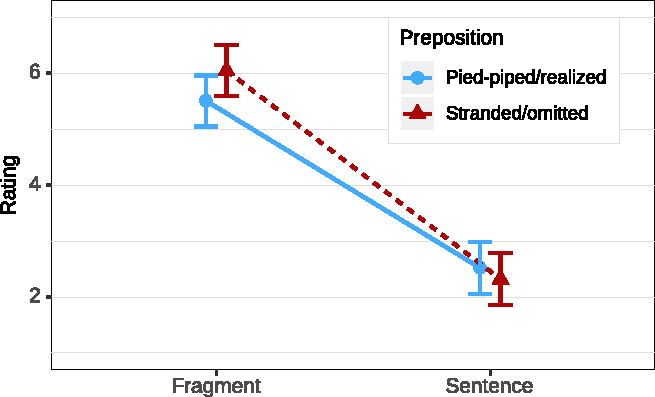
\includegraphics[scale=1]{figures/pst_en_estimates}
 \caption{Mean ratings and 95\% CIs for experiment \ref{exp:pstranding-english}. \label{fig:pstranding-english-estimates}}
\end{figure}

\subsubsection{Results} \label{sec:pstranding-english-results}

Figure \ref{fig:pstranding-english-estimates} provides a summary of the average ratings across conditions. The fragment data show that the omission of the preposition\is{Preposition omission} was slightly more acceptable in English\is{English} \descriptives{6.04}{1.55} than its realization \descriptives{5.5}{1.67}. The sentential left dislocation constructions were heavily degraded across the board no matter whether the preposition was stranded  \descriptives{2.32}{1.43} or pied-piped\is{Pied-piping} \descriptives{2.52}{1.52}. Like in the previous rating studies, the data were analyzed with CLMMs in \texttt{R} following the procedure described in Section \ref{sec:intro-stats}. The full model contained fixed effects for \textsc{Preposition}, \textsc{Sententiality} and \textsc{Position} of the trial in the experiment as well as all two-way interactions thereof. It also contained by-item random intercepts and slopes for \textsc{Preposition}, \textsc{Sententiality} and the interaction thereof and by-subject random intercepts and slopes for \textsc{Preposition}. By-subject random effects for \textsc{Sententiality} were not included, because this IV was tested between subjects. 

\begin{table}[t]
\begin{tabular}{l l l l l l}
\lsptoprule
Predictor & Estimate & SE & $\chi^2$ &  $p$-value &  \\   
\midrule
\textsc{Preposition} & 0.258 &  0.138 & \phantom{1}3.83 & \phantom{\textless}0.062 & \marginal \\
\textsc{Sententiality} & 2.997 &  0.322 & 54.94 & \textless \highsig & ***\\
\textsc{Preposition:Sententiality} & 0.499 &  1 & 11.73 & \textless 0.001 & ***\\
\lspbottomrule
\end{tabular}
\caption{Fixed effects in the final CLMM for experiment \ref{exp:pstranding-english}. \label{tab:pstranding-english-estimates}}
\end{table}

The final model (see Table \ref{tab:pstranding-english-estimates}) contains a significant main effect of \textsc{Sententiality} \clmmLR{54.94}{\highsig}, which shows that short answer fragments\is{Fragment, short answer} are rated\is{Acceptability rating task} better than the presumably underlying left dislocation structures. The marginal main effect of \textsc{Preposition} shows that across the board there is no significant difference between P-stranding\is{Preposition stranding}/PP\is{Preposition phrase} fragments and pied-piping\is{Pied-piping}/DP\is{Determiner phrase} fragments \clmmLR{3.38}{0.06}, but the significant interaction between the two predictors \clmmLR{11.73}{0.001} suggests that specifically in the fragment condition DP\is{Determiner phrase} fragments are more acceptable than PP\is{Preposition phrase} fragments.

\subsubsection{Discussion}
Experiments \ref{exp:pstranding-german} and \ref{exp:pstranding-english} had the purpose of empirically testing the pattern that the PSG\is{P-Stranding Generalization} predicts with respect to preposition omission\is{Preposition omission} in languages with and without P-stranding\is{Preposition stranding}. Taken together, the experiments empirically confirm the pattern that the PSG\is{P-Stranding Generalization} predicts for German\is{German} and English\is{English} short answer fragments\is{Fragment, short answer}. In German\is{German}, omitting the preposition\is{Preposition omission} in the answer is strongly degraded. In contrast, in English\is{English} both DP\is{Determiner phrase} and PP\is{Preposition phrase} fragments are rated\is{Acceptability rating task} as relatively acceptable, and the omission of the preposition\is{Preposition omission} is actually preferred over its realization. This is in line with the prediction that omitting the preposition\is{Preposition omission} in short answers\is{Fragment, short answer} is degraded in languages that lack P-stranding\is{Preposition stranding}, but at least as acceptable as realizing it in languages that allow for this syntactic operation.

The English\is{English} data from experiment \ref{exp:pstranding-english}, however, also show that all of the left dislocation structures that underlie fragments according to movement and deletion\is{Movement and deletion account} are strongly degraded. Furthermore, there is a significant interaction between \textsc{Sententiality} and \textsc{Preposition}: Contrary to what \citet{merchant2004} predicts, the preference for omitting the preposition\is{Preposition omission} in fragments does not match the acceptability of the corresponding left dislocation structures. This observation can be reconciled with the PSG\is{P-Stranding Generalization} if the exceptional movement\is{Exceptional movement account} version of the theory \citep{weir2014} is assumed, which, however, does not predict a strict parallelism between fragments and left dislocation. Given the discussion on pied-piping\is{Pied-piping} in the introduction to this section, \citet{weir2014} would have to explain pied-piping\is{Pied-piping} as the result of a ban on extracting PPs\is{Preposition phrase} which are the complement of a preposition \citep{abels2003, abels2012}. In that case, fronting the complete PP is the only way to evacuate focused constituents from the ellipsis site \citep{heck2008}.

The PSG\is{P-Stranding Generalization} does not explain why omitting the preposition\is{Preposition omission} is preferred in my materials in English\is{English}. A possible reason for this could be that this is due to P-stranding\is{Preposition stranding} in the question. This could either reflect a general preference for omitting the preposition\is{Preposition omission} whenever it is given in the question (this is not possible in German\is{German}), or be an effect of question-answer congruence, as already hinted at above. I return to this question in experiment \ref{exp:pstranding-production}.

The data also have implications for the other theories of fragments discussed in Chapter \ref{sec:chapter-theories}. For the nonsentential and \textit{in situ} deletion\is{In situ deletion account} accounts, the challenge is to provide an explanation for the data from experiments \ref{exp:pstranding-german} and \ref{exp:pstranding-english} that does not rely on movement. Experiments \ref{exp:pstranding-defaultcase} and \ref{exp:pstranding-production} test such non-movement accounts of the preposition omission\is{Preposition omission} data, which are based on case checking\is{Case feature} (experiment \ref{exp:pstranding-defaultcase}) and a nonsyntactic parallelism between question and answer (experiment \ref{exp:pstranding-production}). Empirical evidence for either of these hypotheses would leave movement-based accounts\is{Movement and deletion account} without an explanatory benefit over the simpler \textit{in situ} deletion\is{In situ deletion account} account.

The results also tentatively speak against the claim by \citet{bergen.goodman2015}\is{Ungrammaticality of fragments} that fragments are ungrammatical. Since the missing preposition\is{Preposition omission} (as well as the other omitted material) was unambiguously retrievable from the question, their account does not predict a crosslinguistic difference between English\is{English} and German\is{German} with respect to the acceptability of DP\is{Determiner phrase} fragments. In fact, if all that matters is whether the hearer can retrieve the omitted material, preposition omission might be expected to be \textit{more} acceptable in German\is{German} than in English\is{English}, because the German\is{German} DP\is{Determiner phrase} has prepositional case\is{Prepositional case} marking which restricts the set of possible prepositions. For instance, a hearer who encounters a dative\is{Dative case} DP\is{Determiner phrase} fragment can figure out that the missing preposition must be among those requiring dative\is{Dative case}, whereas such a cue is not available in English\is{English}. This prediction is therefore disconfirmed by the data. This argument of course does not neglect the relevance of information-theoretic\is{Information theory} and processing-based\is{Processing effort} factors to the acceptability and usage of fragments. The experiments in Chapter \ref{sec:chapter-infotheory-experiments} show that predictability plays an important role in the choice between omitting and realizing words.

\refstepcounter{expcounter}\label{exp:pstranding-defaultcase}
\subsection{Experiment \ref{exp:pstranding-defaultcase}: Preposition omission and case}
\label{sec:pstranding-defaultcase}
\subsubsection{Background}
Experiment \ref{exp:pstranding-defaultcase} investigates how acceptable\is{Acceptability rating task} nominative\is{Nominative case} DP\is{Determiner phrase} short answers\is{Fragment, short answer} are as compared to PP\is{Preposition phrase} and prepositional case\is{Prepositional case}-marked DP\is{Determiner phrase} short answers\is{Fragment, short answer} in German\is{German}. This tests two predictions by movement and deletion\is{Movement and deletion account} and the nonsentential account\is{Nonsentential account} of fragments:  First, movement and deletion\is{Movement and deletion account} predicts that nominative\is{Nominative case} DP\is{Determiner phrase} fragments are grammatical as answers to PP\is{Preposition phrase} questions when they can be derived from a cleft\is{Cleft}. Second, the nonsentential account\is{Nonsentential account} also predicts nominative\is{Nominative case} fragments to be acceptable in such contexts: Nominative is the default case\is{Default case} in German\is{German} and does not need to be checked by a preposition. Under both of these lines of reasoning it is expected that PP\is{Preposition phrase} fragments are grammatical, that nominative\is{Nominative case} DP\is{Determiner phrase} fragments are relatively acceptable because they are grammatical, and that prepositional case\is{Prepositional case}-marked DP\is{Determiner phrase} fragments are ungrammatical. According to movement and deletion\is{Movement and deletion account}, their derivation involves ungrammatical P-stranding\is{Preposition stranding}  and according to the nonsentential account\is{Nonsentential account}, prepositional case\is{Prepositional case}-marked DP\is{Determiner phrase} fragments contain a strong uninterpretable case feature\is{Case feature}.

\citet{barton.progovac2005} do not explicitly discuss the status of the PSG\is{P-Stranding Generalization} as evidence for movement, but they observe a crosslinguistic difference between English\is{English} and Serbian\is{Bosnian/Croatian/Serbian} with respect to the possibility of omitting prepositions \is{Preposition omission} in telegraphese utterances. At the example of \Next, \citet[88,89]{barton.progovac2005} show that prepositions can be omitted in English\is{English} sentences like \Next[a], whereas they are obligatory in the Serbian\is{Bosnian/Croatian/Serbian} example \Next[b]. As Serbian\is{Bosnian/Croatian/Serbian} lacks P-stranding\is{Preposition stranding} \citep[667--668]{merchant2004}, this pattern resembles the PSG\is{P-Stranding Generalization}. However, preposition omission\is{Preposition omission} occurs \textit{in situ} in \Next, so the pattern cannot be explained by a restriction\is{Movement restriction} on extracting a DP\is{Determiner phrase} out of the PP\is{Preposition phrase}, like \citet{merchant2004} proposes for preposition omission\is{Preposition omission} in short answers\is{Fragment, short answer}. Whatever blocks the omission in Serbian\is{Bosnian/Croatian/Serbian} must be independent from movement. Note also that these data are highly relevant to the \textit{in situ} deletion\is{In situ deletion account} account, because they show that omitting a preposition\is{Preposition omission} when the remnant is a prepositional case\is{Prepositional case}-marked DP\is{Determiner phrase} can be ruled out even \textit{in situ}.

\ex. \a. Please pick me up (at) Summerside Motel.
\bg. Vidimo se *(na) JFK aerodrom-u.\\
see.\textsc{1pl} Reflexive \phantom{*(}on JFK airport.\textsc{loc}\\
\trans{See you (at) JFK airport.}

\citet{barton.progovac2005} argue that the independent factor that blocks the omission of the preposition\is{Preposition omission} in Serbian\is{Bosnian/Croatian/Serbian} is case checking\is{Case feature}: English\is{English} case features\is{Case feature} are weak and can remain unchecked, whereas Serbian\is{Bosnian/Croatian/Serbian} has strong case features\is{Case feature}, which must be checked. According to \citeauthor{barton.progovac2005}, the strength of Serbian\is{Bosnian/Croatian/Serbian} case features is evidenced by the morphological marking of case. Note that this requires an analysis of prepositional\is{Prepositional case} locative case in \Last[b] as structural case\is{Structural case}, because inherent\is{Inherent case} case can always remain unchecked according to the nonsentential account\is{Nonsentential account}. I return to this issue below. In contrast to the ungrammatical \Last[b], \citeauthor{barton.progovac2005} observe that the preposition can be omitted\is{Preposition omission} in Serbian\is{Bosnian/Croatian/Serbian} when the DP\is{Determiner phrase} appears in nominative\is{Nominative case} case, which they argue is default case\is{Default case} \Next. As they pursue a nonsentential account\is{Nonsentential account}, they do not assume that examples like \Next or the English\is{English} \Last[a] involve the deletion of the preposition, but analyze the noun phrase\is{Noun phrase} as a bare NP\is{Noun phrase}, which simply appears in default case\is{Default case}. Omitting the preposition\is{Preposition omission} is licensed because it is recoverable ``from the verb and the rest of the clause'' \citep[89]{barton.progovac2005}.

\exg. Vidimo se, JFK aerodrom.  \\
see.\textsc{1pl} Reflexive  JFK airport.\textsc{nom}\\
\trans{See you, JFK airport.} \exsourceraised{\citep[89]{barton.progovac2005}}

\largerpage
If the contrast in \LLast could be generalized crosslinguistically, these data would provide a non-movement explanation for the PSG\is{P-Stranding Generalization}: The preposition cannot be omitted\is{Preposition omission} in languages that have prepositional case\is{Prepositional case} marking, but it can in languages that do not, because prepositional case\is{Prepositional case} must be checked by an overt preposition. Interestingly, most of the languages that lack P-stranding\is{Preposition stranding} according to \citet{merchant2004}, such as German\is{German} and Slavonic languages, have prepositional case\is{Prepositional case} marking.%
%
\footnote{This is not true for all of the languages that allow DP\is{Determiner phrase} short answers\is{Fragment, short answer} to PP\is{Preposition phrase} questions according to \citet{merchant2004}. Icelandic\is{Icelandic} has morphological case marking and still allows for P-stranding\is{Preposition stranding} and omission in short answers\is{Fragment, short answer}, whereas Hebrew\is{Hebrew} has no morphological case marking and no P-stranding\is{Preposition stranding}. In the case of Hebrew\is{Hebrew} this could be due to the incorporation of the preposition by the noun. %
}\afterfn%
%
I anticipated above that this reasoning requires that prepositional case\is{Prepositional case} is analyzed as structural case.%
% 
\footnote{
This has been explicitly claimed by \citet[24]{dendikken2013}. In his minimalist\is{Minimalist program} approach, prepositional case\is{Prepositional case} is checked by the head of a functional projection in the PP\is{Preposition phrase} layer and not by P itself. The layer relies crucially on the presence of the preposition, hence prepositional case\is{Prepositional case} is licensed only if the preposition is present.}\afterfn%
%
At least in German\is{German}, this seems to be correct. In Section \ref{sec:theories-predictions-case} I defined structural case\is{Structural case} as a purely linguistic device that makes no significant contribution to meaning. In contrast, inherent\is{Inherent case} case makes such contributions by encoding a specific \texttheta-role. Whether a specific prepositional case\is{Prepositional case} encodes aspects of meaning is an empirical issue. In German\is{German} for instance, there is a tendency for dative\is{Dative case} prepositional case\is{Prepositional case} to mark locations or sources and for accusative\is{Accusative case} to mark goals \citep[8]{zwarts2005}. Still, this relationship is not systematic, because a dative\is{Dative case} DP\is{Determiner phrase} can encode a source \Next[a] as well as a goal \Next[b] and location \Next[c] depending on the preposition it appears with. Taken together, just like I argued in Section \ref{sec:theories-predictions-case} for accusative\is{Accusative case}, prepositional case behaves rather like structural than like inherent\is{Inherent case} case, because it is not strictly associated with a specific \texttheta-role. Even though in German the dative prepositional case\is{Dative case} might be likely to mark the location of an event, it does not always convey this aspect of meaning, unlike inherent\is{Inherent case} dative\is{Dative case}, which marks the recipient.

\ex. \ag. Er rannte aus dem Park.\\
he ran  out the.\textsc{dat} park\\
\trans{He ran out of the park.}  \exsourceraised{\citep[5]{zwarts2005}}
\bg. Er rannte zum Park.\\
he ran to-the.\textsc{dat} park\\
\trans{He ran to the park.} \exsourceraised{\citep[5]{zwarts2005}}
\cg. Er spielte im Park Badminton.\\
he played in-the.\textsc{dat} park badminton\\
\trans{He played badminton in the park.}

If prepositional case\is{Prepositional case} is thus not semantically interpretable, it requires an overt licensor just like other instances of structural case\is{Structural case} do in \citeauthor{barton.progovac2005}'s framework.%
%
\footnote{\citet[342]{progovac.etal2006} argue that a specific prepositional case\is{Prepositional case}, like accusative\is{Accusative case} in the Serbian\is{Bosnian/Croatian/Serbian} example \Next, is acceptable in fragments if it can also be used as inherent\is{Inherent case} case encoding a \texttheta-role. Nevertheless, non-prepositional accusative\is{Accusative case} is associated with the \textsc{Patient} \texttheta-role, so that the fragment is assigned a misleading interpretation if the preposition is omitted\is{Preposition omission}. 

\ex. \ag. Na čega je Stefan seo?\\
	      on what did Stefan sit\\
	      \trans{What did Stefan sit on?} \exsourceraised{\citep[342]{progovac.etal2006}}
	 \bg. *(Na) stolicu.\\
	      on chair.\textsc{acc}\\
	      \trans{(On) a chair.}
	      
Note however that this accounts only for prepositional case\is{Prepositional case} that is otherwise inherent\is{Inherent case}, such as dative\is{Dative case} and genitive\is{Genitive case} in German\is{German}. As I argued above in Section \ref{sec:theories-predictions-case}, there are good reasons not to analyze German\is{German} accusative\is{Accusative case} as inherent\is{Inherent case} (possibly in contrast to Serbian\is{Bosnian/Croatian/Serbian}), so that this explanation does not immediately concern my experiments.}\afterfn%
%
The nonsentential account\is{Nonsentential account} can hence explain at least a large part of the preposition omission\is{Preposition omission} data without assuming unarticulated linguistic structure, actually \textit{because} of the assumption that there is no unarticulated material in fragments that could check the uninterpretable case features\is{Case feature}.%
% 
\footnote{\citet{barton.progovac2005} do not discuss sluicing\is{Sluicing}, therefore it remains open whether they would make a similar prediction for the phenomenon that originally motivated the PSG\is{P-Stranding Generalization}.}\afterfn%
%

Experiment \ref{exp:pstranding-defaultcase} tests this prediction by collecting acceptability ratings\is{Acceptability rating task} for three types of short answer fragments\is{Fragment, short answer} in German\is{German}: PP\is{Preposition phrase} fragments, prepositional case\is{Prepositional case}-marked DP\is{Determiner phrase} fragments and default case-marked DP\is{Determiner phrase} fragments. German\is{German} does not allow for P-stranding\is{Preposition stranding}, it has prepositional case\is{Prepositional case} marking (accusative\is{Accusative case}, dative\is{Dative case} and genitive\is{Genitive case}) as well as nominative\is{Nominative case} default case that never appears as prepositional case\is{Prepositional case}. The nonsentential account\is{Nonsentential account} makes in principle the same predictions as the PSG\is{P-Stranding Generalization} does for PP\is{Preposition phrase} and prepositional case\is{Prepositional case}-marked DP\is{Determiner phrase} fragments: PP\is{Preposition phrase} fragments \Next[a] are expected to be acceptable and prepositional case\is{Prepositional case}-marked DP\is{Determiner phrase} fragments \Next[b] to be degraded. However, the theories disagree on the acceptability of default case DP\is{Determiner phrase} fragments \Next[c]. The nonsentential account\is{Nonsentential account} predicts them to be acceptable, because default case does not need to be checked and the preposition can be easily retrieved from the question. Any sentential account however predicts in principle that the form of the answer matches that of the question, so nominative\is{Nominative case} DP\is{Determiner phrase} fragments will be degraded as compared to PP\is{Preposition phrase} fragments. 

\exg.  Für wen ist das Päckchen?\label{ex:pstranding-defaultcase-sample-item}\\
     for who.\textsc{acc} is the package\\
    \trans{For whom is the package?}
    \ag. Für meinen Vater.\\
     for my.\textsc{acc} father\\
     \trans{For my father.}\exsourceraised{PP}
\bg. Meinen Vater. \\
     my.\textsc{acc} father\\
     \trans{My father.}\exsourceraised{DP, prepositional case}\is{Prepositional case}
 \cg. Mein Vater. \\
     my.\textsc{nom} father\\
     \trans{My father.}\exsourceraised{DP, nominative\is{Nominative case} case}

This does neither imply that the nonsentential account\is{Nonsentential account} predicts nominative\is{Nominative case} DP\is{Determiner phrase} fragments to be as acceptable as PP\is{Preposition phrase} fragments, nor that sentential accounts predict nominative\is{Nominative case} DP\is{Determiner phrase} fragments to be as degraded as prepositional case\is{Prepositional case}-marked DP\is{Determiner phrase} fragments. As for the nonsentential account\is{Nonsentential account}, \citet{progovac.etal2006} argue that even though default case\is{Default case} DP\is{Determiner phrase} fragments are grammatical, they might still be dispreferred for pragmatic reasons. They exemplify this with  \Next, for which they claim that nominative\is{Nominative case} is degraded, because the speaker could have chosen the matching accusative\is{Accusative case} fragment (recall that \citet{progovac.etal2006} claim that the Serbian\is{Bosnian/Croatian/Serbian} accusative\is{Accusative case} is inherent\is{Inherent case} case). Therefore, nominative\is{Nominative case} DP\is{Determiner phrase} fragments might be worse than PP\is{Preposition phrase} fragments, but the nonsentential account\is{Nonsentential account} predicts them to be better than structural case\is{Structural case}-marked DP\is{Determiner phrase} fragments, which are blatantly ungrammatical.

\ex. \ag. Koga je Ana posetila?\\
who.\textsc{acc} is Ana visited \\
\trans{Who did Ana visit?}\exsourceraised{\citep[340]{progovac.etal2006}}
\bg. Vera!\\
Vera.\textsc{nom}\\

In contrast, according to the sentential account, the acceptability of a fragment depends on the availability of a matching antecedent. For instance, nominative\is{Nominative case} would be acceptable if subjects formed a (highly marked) cleft\is{Cleft}ed structure, that requires nominative\is{Nominative case} on the DP\is{Determiner phrase}, as implicit antecedent. Anticipating the results of the experiment,  nominative\is{Nominative case} is rated\is{Acceptability rating task} as even worse than accusative\is{Accusative case}, so this theoretical possibility does not need to be further discussed.

\exg. Es ist mein Vater, für den das Päckchen ist.\\
      it is my.\textsc{nom} father for who.\textsc{acc} the package is\\
      \trans{It's my father, for whom the package is.}

\largerpage[2]
\subsubsection{Materials}
The stimuli were identical to those used in experiment \ref{exp:pstranding-german} except for the additional nominative\is{Nominative case} DP\is{Determiner phrase} fragment condition. The three conditions are exemplified in \ref{ex:pstranding-defaultcase-sample-item} above. As compared to experiment \ref{exp:pstranding-german}, one further item was added in order to present each of the three conditions equally often to the participants.

\subsubsection{Procedure}
The experiment was conducted over the Internet using the LimeSurvey presentation software and completed by 48 participants recruited on the \textit{clickworker} crowdsourcing platform. Each participant was paid \currencyEuro{4.00} for their participation. Subjects were asked to rate the naturalness of the italicized short answer fragment\is{Fragment, short answer} in the context of the question on a 7-point Likert scale (7 = fully natural). Materials were mixed with 24 items from experiment \ref{exp:scripts-rating} and 44 fillers. Both the materials from experiment \ref{exp:scripts-rating} and the fillers resembled the items of experiment \ref{exp:pstranding-defaultcase} in having a context story and an italicized target utterance which subjects rated\is{Acceptability rating task}. Subjects were assigned to one of six lists, to which materials were allocated by a Latin square so that each subject saw each token set only once and each condition equally often. Each two of these lists contained the same materials for experiment \ref{exp:pstranding-defaultcase}, but differed with respect to the materials from experiment \ref{exp:scripts-rating}. All lists were presented in an individually pseudo-randomized order that ensured that no two items or fillers of the same category immediately followed each other. Three subjects rated\is{Acceptability rating task} more than the previously established threshold of two out of five ungrammatical controls as natural (6 or 7 points) and thus were excluded from further analysis.

\subsubsection{Results} 
Table \ref{tab:p-case-means} summarizes the ratings for the three conditions. The ratings for PP\is{Preposition phrase} and prepositional case\is{Prepositional case}-marked DP\is{Determiner phrase} fragments replicate the previous studies. Nominative\is{Nominative case} DP\is{Determiner phrase} fragments are perceived as even less acceptable than prepositional case\is{Prepositional case}-marked DP\is{Determiner phrase}s.

\begin{table}[t]
 \begin{tabular}{l l l l}
 \lsptoprule
  Condition &  Exp. \ref{exp:pstranding-defaultcase} & Exp. \ref{exp:pstranding-german} & \citet{merchant.etal2013}\\
 \midrule
 PP\is{Preposition phrase} & 6.31 (1.18) & 6.61 (0.99)& 5.99 (1.64)\\
DP\is{Determiner phrase}, Structural case & 4.81 (1.99)&4.42 (2.05)& 4.76 (2.03)\\
DP\is{Determiner phrase}, Nominative\is{Nominative case} & 3.57 (1.96)& -- & -- \\
\lspbottomrule
 \end{tabular}
  \caption{Mean ratings (standard deviation) by condition in experiment \ref{exp:pstranding-defaultcase}, in experiment \ref{exp:pstranding-german} and in the P-stranding study by \citet{merchant.etal2013}\label{tab:p-case-means}. \textit{Structural case} refers to prepositional case in experiment \ref{exp:pstranding-defaultcase} and accusative in the other two studies.}
 \end{table}

The data were analyzed with CLMMs in \texttt{R} following the procedure described in Section \ref{sec:intro-stats}. In this case, the procedure slightly differed from that applied to previous studies, because the IV was a nominal-scaled factor with three levels. The likelihood ratio tests used for model selection only allow for the comparison of two models containing or lacking a factor and but not for pairwise comparisons between the individual levels. Therefore, I created two subsets from the complete data set in order to compare the factor levels  pairwise. I first compared only the PP\is{Preposition phrase} to the prepositional case\is{Prepositional case}-marked DP\is{Determiner phrase} fragments, thus replicating experiment \ref{exp:pstranding-german}. Then I tested whether the nominative\is{Nominative case} and prepositional case\is{Prepositional case}-marked DP\is{Determiner phrase} fragments differed significantly in acceptability\is{Acceptability rating task} by analyzing these conditions only. This procedure allows for pairwise comparisons between factor levels and not only for testing whether including a factor as a whole improves model fit. For both subsets I started with a full model containing fixed effects for \textsc{FragmentType}, the \textsc{Position} of the trial in the experiment and their interaction and by-item and by-subject random intercepts and random slopes for each predictor. The final models (see Tables \ref{tab:pst-case-estimates-pp-str} and \ref{tab:pst-case-estimates-str-def}) show that all contrasts between the levels of \textsc{FragmentType} are significant. PP\is{Preposition phrase}s are rated\is{Acceptability rating task} significantly better than case-marked DP\is{Determiner phrase}s \clmmLR{29.18}{\highsig} and nominative\is{Nominative case} case-marked DP\is{Determiner phrase}s are even worse than prepositional case\is{Prepositional case}-marked DP\is{Determiner phrase}s \clmmLR{15.37}{\highsig}. In the model that compared PP\is{Preposition phrase}s to prepositional case\is{Prepositional case}-marked DP\is{Determiner phrase} fragments there was also a significant \textsc{Position} effect, which did not interact with \textsc{FragmentType}.

\begin{table}[t]
\begin{tabular}{l l l l l l}
\lsptoprule
Predictor & Estimate & SE & $\chi^2$ &  $p$-value &  \\   
\midrule
\textsc{FragmentType} & 2.58 & 0.423 &  15.37 & \textless \highsig& ***\\
\textsc{Position} &  0.01 & 0.004 &  \phantom{1}4.34  &  \textless 0.05& *\\
\lspbottomrule
\end{tabular}
 \caption{Fixed effects in the final model comparing PP fragments to prepositional case-marked DP fragments.\label{tab:pst-case-estimates-pp-str}}
\end{table}

\begin{table}[t]
\begin{tabular}{l l l l l l}
\lsptoprule
Predictor & Estimate & SE & $\chi^2$ &  $p$-value &  \\   
\midrule
\textsc{FragmentType} & 1.838 & 0.414 & 29.18 & \textless \highsig &***\\
\lspbottomrule
\end{tabular} 
\caption{Fixed effects in the final model comparing prepositional case-marked DP fragments to nominative DP fragments.\label{tab:pst-case-estimates-str-def}}
\end{table}

\subsubsection{Discussion}
Experiment \ref{exp:pstranding-defaultcase} tested whether nominative\is{Nominative case} DP\is{Determiner phrase} fragments are more acceptable than prepositional case\is{Prepositional case}-marked DP\is{Determiner phrase} fragments, and how they are rated\is{Acceptability rating task} in comparison to PPs\is{Preposition phrase}. Both the nonsentential account\is{Nonsentential account} \citep{barton.progovac2005} and the movement and deletion\is{Movement and deletion account} account predict a preference for nominative\is{Nominative case} DP\is{Determiner phrase}s over case-marked ones, but for independent reasons. According to the nonsentential account\is{Nonsentential account}, prepositions can be omitted\is{Preposition omission} in short answer fragments\is{Fragment, short answer} only if they are not required for checking prepositional case\is{Prepositional case}. The nonsentential account\is{Nonsentential account} predicts fragments in nominative\is{Nominative case} default case to be acceptable under such circumstances. According to the movement and deletion\is{Movement and deletion account} account, DP\is{Determiner phrase} short answers might be grammatical as answers to PP questions in German\is{German} when they can be derived from a cleft\is{Cleft}. In that case, the DP\is{Determiner phrase} must exhibit nominative\is{Nominative case} case morphology. 

The experiment disconfirms these predictions: Nominative\is{Nominative case} DP\is{Determiner phrase} fragments are significantly less acceptable than prepositional case\is{Prepositional case}-marked ones. PP\is{Preposition phrase} short answers\is{Fragment, short answer} are even more strongly preferred than prepositional case\is{Prepositional case}-marked DP\is{Determiner phrase}s. This finding challenges the cleft\is{Cleft}-based analysis of apparent preposition omission\is{Preposition omission} under ellipsis in languages that lack P-stranding\is{Preposition stranding}. In a language with overt case marking, like German\is{German}, such an account predicts that DP\is{Determiner phrase} fragments derived from clefts\is{Cleft} by ellipsis appear in nominative, just like in the corresponding full sentences. Even though the movement and deletion\is{Movement and deletion account} account does not predict that the resulting nominative DP\is{Determiner phrase} fragments are as acceptable as PP\is{Preposition phrase}s (they might be degraded for pragmatic reasons), they are expected to be more acceptable than prepositional case\is{Prepositional case}-marked DP\is{Determiner phrase}s, which it analyzes as being derived only by ungrammatical P-stranding\is{Preposition stranding}. This prediction is clearly disconfirmed by the experiment, since this predicted acceptability\is{Acceptability rating task} pattern is inverted in the data.

\largerpage
From the perspective of the nonsentential account\is{Nonsentential account}, the contrast to the English\is{English} data from experiment \ref{exp:pstranding-english}, which revealed a preference for preposition omission\is{Preposition omission}, is particularly striking. If the explanation for the English\is{English} pattern is that the preposition can be omitted\is{Preposition omission} because it is given in the question and the resulting nominative\is{Nominative case} DP\is{Determiner phrase} fragment does not require case checking\is{Case feature}, the same pattern is expected for German\is{German} default case\is{Default case} (nominative\is{Nominative case}) DP\is{Determiner phrase} fragments. Therefore, experiment \ref{exp:pstranding-defaultcase} strongly suggests that the nonsentential case checking\is{Case feature} account should be rejected. Sentential accounts predict connectivity effects\is{Case connectivity} between question and answer, and consequently are in line with the preference for realizing the preposition in the answer as well. 

\noindent The gradual acceptability\is{Acceptability rating task} cline between the three short answer\is{Fragment, short answer} types is in line with the idea that fragments are ungrammatical but can be interpreted after applying a probabilistic repair mechanism, as \citet{bergen.goodman2015}\is{Ungrammaticality of fragments} suggest. The prepositional case\is{Prepositional case}-marked DP\is{Determiner phrase} fragments are clearly dispreferred in all three experiments and are therefore degraded in the context of PP\is{Preposition phrase} questions in German\is{German}. Nonetheless, prepositional case\is{Prepositional case} can function as a probabilistic cue that points toward the preposition that is missing. Since prepositional case\is{Prepositional case} is determined by the preposition, processing a dative\is{Dative case} DP\is{Determiner phrase} will restrict the range of possible prepositions to those requiring dative\is{Dative case}. Nominative\is{Nominative case} DP\is{Determiner phrase} fragments could be rated\is{Acceptability rating task} worse because they lack this cue. Under this perspective, both case-marked and default case\is{Default case} DP\is{Determiner phrase} fragments are ungrammatical, because they lack an appropriate antecedent. The acceptability difference between these ungrammatical utterances could be explained by the effort\is{Processing effort} required to figure out which part of the utterance is missing. However, the comparison between English\is{English} and German\is{German} in experiments \ref{exp:pstranding-german} and \ref{exp:pstranding-english} shows that the recoverability of the preposition cannot be the whole story. Its omission\is{Preposition omission} is less acceptable in German\is{German} despite the fact that English\is{English} lacks prepositional case\is{Prepositional case} as a cue toward in the omitted preposition\is{Preposition omission}. Consequently, the preference for prepositional case\is{Prepositional case} in comparison to default case\is{Default case} might be due to differences in recoverability of the omitted preposition\is{Preposition omission}, but the inverted preference for DP\is{Determiner phrase} and PP\is{Preposition phrase} short answer\is{Fragment, short answer}s between German\is{German} and English\is{English} must receive a different explanation. 

Taken together, experiment \ref{exp:pstranding-defaultcase} disconfirms the case checking\is{Case feature}-based account that follows from the discussion on preposition omission\is{Preposition omission} in \citet{barton.progovac2005}. The experiment also showed that nominative\is{Nominative case} DP\is{Determiner phrase} fragments, which might be derived from cleft\is{Cleft} structures according to movement and deletion\is{Movement and deletion account} are more strongly degraded than presumably ungrammatical DP\is{Determiner phrase}s in prepositional case\is{Prepositional case}. The relative acceptability of these DP\is{Determiner phrase}s as compared to nominative\is{Nominative case} ones, which all of the theories can derive, suggests that they might not be fully ungrammatical but dispreferred for independent reasons. Experiment \ref{exp:pstranding-production} addresses this issue.

\refstepcounter{expcounter}\label{exp:pstranding-production}
\subsection{Experiment \ref{exp:pstranding-production}: Question-answer parallelism}
\label{sec:pstranding-production}

\subsubsection{Background}
\label{sec:pstranding-production-background}

Experiment \ref{exp:pstranding-production} tests the hypothesis that the availability of P-stranding\is{Preposition stranding} and of preposition omission\is{Preposition omission} in a language often cooccur due to a nonsyntactic relationship between question and answer. If this hypothesis were confirmed, the data that \citet{merchant2004} interprets as evidence for movement\is{Movement and deletion account} in fragments could be explained without assuming that movement is required as an explanatory link between the acceptability of fragments and the availability of P-stranding\is{Preposition stranding}.

\is{Fragment, short answer|(}\is{Preposition omission|(}The data discussed so far are in line with the PSG\is{P-Stranding Generalization}: Experiments \ref{exp:pstranding-german} and \ref{exp:pstranding-english} confirm its predictions for English\is{English} and German\is{German} and experiment \ref{exp:pstranding-defaultcase} rules out the alternative nonsentential account\is{Nonsentential account} based on case checking\is{Case feature}. However, parallelisms between fragments and movement constructions support the movement and deletion\is{Movement and deletion account} account only if derivationally simpler theories, like the nonsentential\is{Nonsentential account} and \textit{in situ} deletion\is{In situ deletion account} accounts, cannot explain the data as well. In the case of the PSG\is{P-Stranding Generalization}, there are at least three possible explanations for the data: First, as \citet{merchant2004} argues, they could of course evidence a genuine movement restriction\is{Movement restriction}. Second, there could be an independent factor that blocks the omission of the preposition\is{Preposition omission} in languages that disallow P-stranding\is{Preposition stranding}. The nonsentential case checking\is{Case feature} hypothesis that I tested in the previous section is an example for this line of reasoning. Even though I rejected this explanation, the impossibility of omitting prepositions\is{Preposition omission} in German\is{German} (as compared to English\is{English}) in \textit{in situ} contexts might still evidence such a different independent factor other than the one I tested in experiment \ref{exp:pstranding-defaultcase}.%
%
\footnote{For instance, \citet[21]{zwarts2005} claims that preposition and case are ``not two semantically independent elements'' in German\is{German}, but that they are interpreted together. Another such factor could be crosslinguistic differences with respect to feature percolation\is{Feature percolation}. If a focus feature percolated from the DP\is{Determiner phrase} to PP\is{Preposition phrase} obligatorily in German\is{German} but not in English\is{English}, e.g. due to PP\is{Preposition phrase}-internal movement operations required for case checking\is{Case feature}, the \textit{in situ} deletion\is{In situ deletion account} account could explain why the omission of the preposition\is{Preposition omission} is blocked in languages that do not allow for P-stranding\is{Preposition stranding}.}\afterfn%
% 

A third possibility, which experiment \ref{exp:pstranding-production} explores, is that there is no structural difference between English\is{English} and German\is{German} PPs\is{Preposition phrase} that blocks the omission of the preposition\is{Preposition omission} in fragments, but that the form of the \textit{wh}-phrase in the question constrains that of the answer\is{Fragment, short answer}: If the preposition is pied-piped\is{Pied-piping} in the question, it must be realized in short answers\is{Fragment, short answer}, and if it is stranded in the question, it is omitted\is{Preposition omission} in the answer\is{Fragment, short answer}. From this perspective, preposition omission\is{Preposition omission} in German\is{German} short answers\is{Fragment, short answer} is not blocked by properties of the answer\is{Fragment, short answer}, but dispreferred because of the impossibility of stranding\is{Preposition stranding} the preposition in the question. In principle, both forms of the answer\is{Fragment, short answer} are possible, but one of them is strongly preferred for nonsyntactic reasons.

\noindent Experiment \ref{exp:pstranding-production} tests this hypothesis by eliciting answers to questions with pied-piping\is{Pied-piping} and P-stranding\is{Preposition stranding} in a production study\is{Production task} in English\is{English}, which allows for both forms of the answer. If subjects adapt their answer to the question, they must produce a higher ratio of preposition omission\is{Preposition omission} when the preposition is stranded\is{Preposition stranding} the question and realize it more often in the answer when it is pied-piped\is{Pied-piping}.

This raises the question of why such a mechanism would be observed at all. In the theoretical literature, there are at least two possible explanations that predict a nonsyntactic question-answer parallelism: First, a structured propositions account of question semantics \citep{vonstechow1981, reich2002a} relates the focus structure of question and answer. Second, structural persistence \citep{nykiel2017} between question and answer could result from speakers' tendency to reuse structure from previous discourse \citep{levelt.kelter1982, nykiel2017}. 

\subsubsubsection{Structured propositions}
\label{sec:psg-alternatives-structured}\largerpage[-1]

The central idea of the structured propositions account of question-answer parallelism is that the focus structure of the answer is determined by that of the question \citep{reich2002, reich2002a, reich2007}.%
%
\footnote{Note that this might also be expected under a movement and deletion\is{Movement and deletion account} account. However, if it were the case, the prediction of movement and deletion\is{Movement and deletion account} and \textit{in situ} deletion\is{In situ deletion account} with respect to preposition omission\is{Preposition omission} would be fully aligned: Both theories predict that only words which belong to the focus survive ellipsis, and no matter whether they are previously moved, the outcome is identical. In that case, the PSG\is{P-Stranding Generalization} would not provide genuine evidence for movement. As I showed in Section \ref{sec:pstranding-background-mp}, it does only if the focus structure of pied-piping\is{Pied-piping} and P-stranding\is{Preposition stranding} questions (and the corresponding) answers is identical and pied-piping\is{Pied-piping} occurs because extraction out of PP\is{Preposition phrase} is ungrammatical.}\afterfn%
%
If the preposition in the question is focused, it must also be focused in the answer and therefore cannot be omitted\is{Preposition omission} there. If the preposition is not focused in the question, it also not in the answer, and consequently it can be targeted by ellipsis.%
%
\footnote{See \citet{griffiths2019} for a similar account of the PSG\is{P-Stranding Generalization} data.}\afterfn%
%

\citet{reich2002a} models the semantics of questions as a set of structured propositions, which are sensitive to focus structure \citep{vonstechow1981}. For instance, \citet[82]{reich2002a} defines the semantics of \Next[a] as denoting the set of propositions in \Next[b], which is summarized as \Next[c]. The idea is that, instead of defining the semantics of \Next[a] as a set of unstructured propositions \NNext, the focus, i.e. the \textit{wh}-phrase in \Next, is separated from the background of the question. Congruent answers must match this focus-background structure.

\ex. \a. What did John drive? \hfill \citep[82]{reich2002a}
     \b. $\{\langle Mary's\;red\;convertible, \lambda x.John\;drove\;x \rangle,\\
     \langle Peter's\;Porsche, \lambda x.John\;drove\;x \rangle, \dots\}$
     \c. $\lambda p \exists x [thing'(x)\;\&\;p = \langle x,\;\lambda y.John\;drove\;y\rangle]$
     
\ex. $\lambda x. John\;drove\;x$

\citet{reich2002a} does not address pied-piping\is{Pied-piping}, but in \citet{reich2002} he develops a structured propositions analysis of complex \textit{wh}-phrases. He assumes that the pied-piped\is{Pied-piping} material belongs to the focus in complex \textit{wh}-phrases like \textit{whose book} in \Next[a], whose semantics he defines as \Next[b]. He argues that an answer that does not match this focus-background structure is incongruent, because it is not included in the denotation of the question. Applied to pied-piping\is{Pied-piping} of prepositions, the semantics of a question like \NNext[a] would be defined as \NNext[b], whereas that of the corresponding P-stranding\is{Preposition stranding} question is given in \ref{ex:structural-pstranding}. This requires congruent answers to \NNext and \ref{ex:structural-pstranding} to differ in their focus structure: \ref{ex:structural-pstranding-a-pp} is a congruent answer to \NNext, but \ref{ex:structural-pstranding-a-pst} is not. In the case of a P-stranding question like \ref{ex:structural-pstranding}, the opposite holds.

\newpage
\ex. \a. Whose book did you read?\hfill\citep{reich2002}
    \b. $\{\langle\langle x, \lambda z . z's book \rangle ,\;\lambda y . you\;read\;y \rangle;\; x \; is \; a \; person\}$
    
\ex. \a. With whom did you talk?
    \b. $\{\langle\langle x, \lambda z . with\; z \rangle ,\;\lambda y.\; you\;talk\;y \rangle;\; x \; is \; a \; person\}$

\ex. \label{ex:structural-pstranding}
\a. Who did you talk with?
    \b. $\{\langle\langle x,\;\lambda y.\; you\;talk\;with\;y \rangle;\; x \; is \; a \; person\}$

\ex. \a. \sout{I talked} [with John]\textsubscript{\textsc{F}}.\label{ex:structural-pstranding-a-pp}
     \b.  \sout{I talked with} [John]\textsubscript{\textsc{F}}.\label{ex:structural-pstranding-a-pst}

The assumption that relatively subtle differences in meaning can impact on the form of fragments has recently been reinforced by \citet{weir2018}. He observes that despite the questions in \Next and \NNext being relatively meaning-equivalent, fragments that do not match the semantics of the \textit{wh}-phrase are heavily degraded.\largerpage

\ex. \label{ex:weir-qa-ex1}
 Q: How many signals did the machine send? \hfill \citep[1289]{weir2018}
\a.  \a. It sent \textsc{two} signals.
\b. ?It sent a signal \textsc{twice}.
\z.
\b. \a. \textsc{two} (signals).
\b. *\textsc{twice}.
\z.

\ex. \label{ex:weir-qa-ex2}
Q: How many times did the machine send a signal? \hfill \citep[1289]{weir2018}
\a. \a. ?It sent \textsc{two} signals.
    \b. It sent a signal \textsc{twice}.
    \z.
\b.
\a.* \textsc{two} (signals).
\b. \textsc{twice}.
\z.

The structured propositions approach offers a straightforward explanation for the contrast between German\is{German} and English\is{English} with respect to the acceptability of preposition omission\is{Preposition omission} in fragments. Unlike English\is{English}, German\is{German} lacks P-stranding\is{Preposition stranding} in questions, hence questions always involve pied-piping\is{Pied-piping} and only answers where the complete PP\is{Preposition phrase} is focused are congruent. As the central assumption of the \textit{in situ} deletion\is{In situ deletion account} account is that focused expressions survive ellipsis, the preposition can never be omitted\is{Preposition omission} in those contexts. With respect to English\is{English}, where both P-stranding\is{Preposition stranding} and pied-piping\is{Pied-piping} are available, the structured propositions approach predicts a relatively strict congruence between the form of the question and that of the answer. As the contrast between \ref{ex:weir-qa-ex1} and \ref{ex:weir-qa-ex2} suggests, there should be a strong preference for the answer to match the form of the question: Pied-piping\is{Pied-piping} questions are expected to require PP\is{Preposition phrase} short answers\is{Fragment, short answer}, whereas P-stranding\is{Preposition stranding} questions require DPs\is{Determiner phrase}.
\newpage

\subsubsubsection{Structural persistence}
The second account of question-answer parallelism is based on processing\is{Processing effort}. The idea is that both DP\is{Determiner phrase} and PP\is{Preposition phrase} fragments can be derived by the syntax in the context of PP\is{Preposition phrase} questions in English\is{English} and German\is{German}, but that a tendency for speakers to reuse syntactic structure from previous discourse explains why short answer fragments\is{Fragment, short answer} often match the form of the preceding question. This has been proposed by \citet{nykiel2017}, who traces back the observation of a tendency to reuse syntactic structure from previous discourse to \citet{levelt.kelter1982}. \citet{levelt.kelter1982} conducted a series of experiments that investigated how and why speakers reuse structure in the example of the optional omission of prepositions\is{Preposition omission} in Dutch\is{Dutch} questions and answers like \Next, from \citet[80]{levelt.kelter1982}. For this language, they argue that the preposition \textit{aan} `to' can be freely omitted\is{Preposition omission} in the question and the short answer\is{Fragment, short answer} fragment without changing its meaning.

\ex. \ag. (Aan) wie laat Paul zijn viool zien?\\
      to  whom allows Paul his violin see\\
      \trans{Who allows Paul to see his violin?}
      \bg. (Aan) Toos.\\
      to Toos\\
      \trans{Toos.}

Throughout their experiments, \citet{levelt.kelter1982} find an effect of the form of the question on the form of the answer: The preference for omitting the preposition\is{Preposition omission} in the answer is stronger when it is been omitted\is{Preposition omission} in the question and vice versa. Note that \Last does not involve P-stranding\is{Preposition stranding}, but the general idea straightforwardly applies to P-stranding\is{Preposition stranding} data. If speakers reuse the structure given in a P-stranding\is{Preposition stranding} question, they should prefer DP\is{Determiner phrase} fragments, whereas PP\is{Preposition phrase} fragments would be preferred in case of pied-piping\is{Pied-piping} questions. 

This prediction is supported by English\is{English} corpus\is{Corpus} data \citep{nykiel2014, nykiel2017}. \citet{nykiel2017} shows that despite an overall preference for omitting the preposition\is{Preposition omission} in the remnant,%
%
\footnote{\citet{nykiel2017} investigated a more extensive range of antecedents, instead of looking only into question answer pairs. In the case of the latter, the remnant is the short answer\is{Fragment, short answer}.}\afterfn%
%
the rate of DP\is{Determiner phrase} fragments (90\%) is significantly higher when the preposition is stranded\is{Preposition stranding} or omitted\is{Preposition omission} than when the preposition is pied-piped\is{Pied-piping} or appears adjacent to its object (58.8\%). Even though her corpus studies\is{Corpus} are concerned only with English\is{English} data, \citet[41-42]{nykiel2017} argues that her observations for English\is{English} also provide an explanation for the crosslinguistic pattern: If the form of the antecedent (e.g. the PP\is{Preposition phrase} in the question) determines the form of the fragment, DP\is{Determiner phrase} short answers\is{Fragment, short answer} to questions where the \textit{wh}-phrase is the complement of a preposition are only possible when there are DP\is{Determiner phrase} antecedents. In German\is{German} there are never such antecedents because German\is{German} has no P-stranding\is{Preposition stranding}. Consequently, the preposition is never omitted\is{Preposition omission} in the answer.

\subsubsubsection{Predictions of question-answer parallelism}
Both the structured pro\-positions and the structural persistence accounts provide a non-movement explanation for the data that \citet{merchant2001, merchant2004} presents as evidence for the PSG\is{P-Stranding Generalization}. Besides explaining the crosslinguistic data, such an approach predicts that within a language that allows for an alternation between P-stranding\is{Preposition stranding} and pied-piping\is{Pied-piping}, the form of the answer will match that of the question, like \citet{levelt.kelter1982} showed for preposition omission\is{Preposition omission} in Dutch\is{Dutch}.\is{Fragment, short answer|)}

Since the goal of experiment \ref{exp:pstranding-defaultcase} is to investigate whether question-answer parallelism can explain the preposition omission\is{Preposition omission} data without having to assume movement in fragments\is{Movement and deletion account}, the experiment does not need to differentiate between the semantic and the processing accounts. However, the structured propositions account predicts a relatively strict match between question and answer, whereas this relationship might be looser if the structural persistence account is correct. From a semantic perspective, if focusing the preposition in the question blocks its omission\is{Preposition omission} in the answer, the form of the question would strictly determine that of the answer. The tendency to reuse structure might interact with and be overridden by other constraints, such as the tendency to be brief and to omit redundant material.%
%
\footnote{See Section \ref{sec:infotheory-uid} for discussion.}\afterfn%
%
The conclusions on this issue will only be tentative.\largerpage

In contrast to question-answer parallelism, the movement and deletion\is{Movement and deletion account} account does not necessarily predict a correlation between the form of the question and the answer: As I discussed above, if the alternation between DP\is{Determiner phrase} and PP\is{Preposition phrase} short answers\is{Fragment, short answer} is traced back to different focus structures, it does not provide evidence specifically for movement\is{Movement and deletion account}. Consequently, movement and deletion\is{Movement and deletion account} implies that P-stranding\is{Preposition stranding} and pied-piping\is{Pied-piping} questions do not differ with respect to their focus structure. It is important to note that a syntactic theory like the movement and deletion\is{Movement and deletion account} account does not conflict with the assumption of processing constraints\is{Processing effort}, like the structural persistence account. Processing constraints can determine the choice for a particular utterance when grammar allows for various options. However, if an independently evidenced processing constraint can explain the data that the syntactic theory was designed to account for, this syntactic theory yields no explanatory benefit over simpler theories. In that case, the preposition omission\is{Preposition omission} data would lose their status as evidence for movement in fragments\is{Movement and deletion account}.\is{Preposition omission|)}

\subsubsubsection{Approach}
Experiment \ref{exp:pstranding-production} uses a production task\is{Production task} to investigate whether subjects adapt answers to the form of the question. I conducted the study in English\is{English}, which allows for both P-stranding\is{Preposition stranding} and pied-piping\is{Pied-piping}. There is some previous experimental evidence that points into this direction: The corpus studies\is{Corpus} by \citet{nykiel2014, nykiel2017} and the experiments by \citet{levelt.kelter1982} suggest that there is question-answer parallelism, but \citet{levelt.kelter1982} investigate a related yet different phenomenon and \citet{nykiel2014, nykiel2017} considers very diverse antecedents and remnants, such as interrogative fragments and elliptical questions. An experimental study allows for controlling this variance and for testing only pied-piping\is{Pied-piping} and P-stranding\is{Preposition stranding} questions, which are the relevant antecedents given the above discussion on question-answer parallelisms.

In the experiment, subjects read a context story followed by a question with a stranded\is{Preposition stranding} \Next[a] or a pied-piped\is{Pied-piping} \Next[b] preposition and are asked to produce a natural answer to that question. Question-answer parallelism predicts a (relatively) higher rate of DP\is{Determiner phrase} fragments for P-stranding\is{Preposition stranding} questions \Next[a] and a higher rate of PP\is{Preposition phrase} fragments for questions with pied-piping\is{Pied-piping} \Next[b]. 

\ex. Molly and Cooper are colleagues and talk about football during a break. Because this evening there is an important match, Cooper asks Molly:
\a. Who are you rooting for? \hfill P-stranding\is{Preposition stranding}
\b. For whom are you rooting? \hfill Pied-piping\is{Pied-piping}

If subjects provide sentential answers, I expected them to follow the unmarked SVO word order\is{Word order} in \Next[a], because experiment \ref{exp:pstranding-english} suggests that non-con\-tras\-tive object fronting \Next[b,c] is at least highly marked, if not ungrammatical, in English\is{English}.

\ex. \a. I'm rooting for the Packers.
     \b. *For the Packers, I'm rooting.
     \c. *The Packers, I'm rooting for.

\subsubsection{Materials}
All materials followed the pattern given in \LLast: A short context story consisting of two sentences introduced two characters and was followed by a question asked by one of these characters. This question was always a \textit{wh}-question, where the \textit{wh}-phrase was the complement of a preposition. The question was presented in one of two conditions, P-stranding\is{Preposition stranding} \LLast[a] and pied-piping\is{Pied-piping} \LLast[b]. %

\newpage
\noindent I investigated three different types of questions, which differ in the status of the PP\is{Preposition phrase} with respect to the verb. The reason for this is that the choice between the two constructions is not fully unconstrained, but depends on syntactic properties of the PP\is{Preposition phrase}. For instance, \citet[26]{vanriemsdijk1978} argues that P-stranding\is{Preposition stranding} is not possible in adjunct\is{Adjunct} PP\is{Preposition phrase}s, and \citet{nykiel2017} shows that pied-piping\is{Pied-piping} is less frequent the stronger the semantic connection between verb and preposition is. Investigating the reason underlying these contrasts is beyond the goal of the experiment,%
% 
\footnote{But see \citet{vanriemsdijk1978}, \citet{chomsky1981}, \citet{pullum.huddleston2002} and \citet{nykiel2017}.}\afterfn%
%
but if P-stranding\is{Preposition stranding} was blocked or triggered by some syntactic property of the PP\is{Preposition phrase} and this remained uncontrolled it could mask effects of the form of the question. Therefore, I tested questions with non-locative PP\is{Preposition phrase}s which are subcategorized by the verb \LLast, locative complement PP\is{Preposition phrase}s (source / goal / location) \Next[a] and adjunct\is{Adjunct} PP\is{Preposition phrase}s \Next[b]. This will (i) show whether the type of the PP\is{Preposition phrase} affects the preference for P-stranding\is{Preposition stranding} or pied-piping\is{Pied-piping}, and (ii), if this was the case, these preferences can be taken into account in the statistical analysis.

\ex. \a. Where do you come from? \hfill Locative
     \b. For whom did you buy it? \hfill Adjunct\is{Adjunct}

Finally, note that the difference between adjunct\is{Adjunct} and complement is also potentially relevant to the movement and deletion\is{Movement and deletion account} account. If there are movement restrictions\is{Movement restriction} on some PPs\is{Preposition phrase} in English\is{English}, \citet{merchant2004} predicts the fragments derived via illicit movement operations to be less acceptable and therefore to be only rarely produced.

\subsubsection{Procedure} 
53 self-reported native speakers of American English\is{English} were recruited on the \textit{Prolific Academic} crowdsourcing platform. The experiment was conducted over the Internet and presented using the LimeSurvey survey presentation software. Subjects were rewarded \currencyPound{2} for participating. The task consisted in reading the context story and the question and entering the answer that the subject considered to be most natural into a text field. Form and meaning of the answer were totally unconstrained apart from this; specifically, subjects were told to produce an utterance, but there was no restriction with respect to sententiality. Subjects were assigned to one of two lists, to which the materials were distributed with a Latin square. There were 24 items, eight of which had locative PPs\is{Preposition phrase}, eight adjunct\is{Adjunct} PPs\is{Preposition phrase} and eight argument PPs\is{Preposition phrase}. Materials were balanced across lists, so that each subject saw 12 items per \textsc{Question} (P-stranding\is{Preposition stranding}/pied-piping\is{Pied-piping}) condition and within those 12 items per condition there were four of each of the PP types (argument / adjunct\is{Adjunct} / locative). Materials were mixed with 19 items of an unrelated experiment and 25 unrelated fillers and presented in individually pseudo-randomized order that ensured that no two items of the same experiment immediately followed each other. All fillers resembled the items in requiring subjects to produce an answer to a question. The \textit{wh}-phrase was the complement of a preposition in these questions.

The answers were annotated manually. First, it was recorded whether the answer was a direct answer to the question or not. An answer was classified as a direct answer when it contained or consisted in a DP\is{Determiner phrase} or PP\is{Preposition phrase} that corresponded to the \textit{wh}-phrase in the question. This excludes cases such as \Next.

\ex. Who are you rooting for?
\a. I don't really care, I just go for the excitement of it all. 
     \b. I'm a big Pats fan.
     \c. Not sure.
     
The restriction to direct answers excluded a total of 20.1\% of the data. Direct answers were then annotated for two further features. First, I tracked whether the answer was a complete sentence or a fragment\is{Fragment, short answer}. Second, it was annotated whether the preposition was omitted\is{Preposition omission} or realized in fragments and whether it was realized \textit{in situ}, pied-piped\is{Pied-piping} or stranded\is{Preposition stranding} in sentences.

\subsubsection{Results}
Figure \ref{fig:ex8_prod_relfrag} gives an overview of the complete data set. Within the direct sentential answers there was no structural variation at all: As I expected, the PP\is{Preposition phrase} always occurred in its postverbal base position and there was no instance of pied-piping\is{Pied-piping} or P-stranding\is{Preposition stranding}. Therefore, I restricted the further analysis to fragments. Across all conditions, direct fragment answers\is{Fragment, short answer} that could be statistically analyzed made up 55.3\% of the complete data.

\begin{figure}[t]
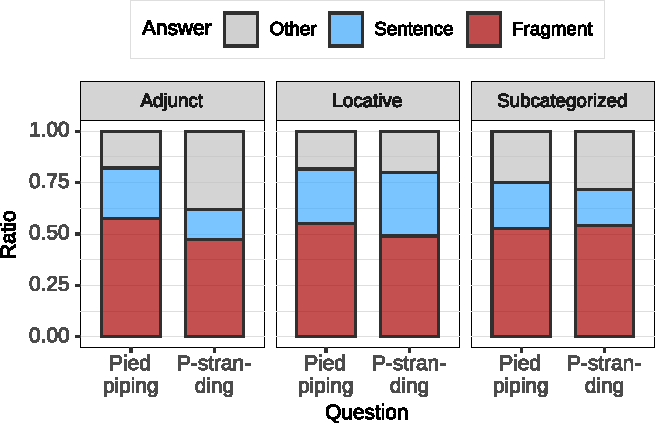
\includegraphics[scale=1]{figures/ex8_prod_answers}
 \caption{Ratios of answer categories in exp. 4. ``Other'' indicates indirect answers or constructions not involving P-stranding/Pied-piping\label{fig:ex8_prod_relfrag}.}
\end{figure}

Figure \ref{fig:ex8_prod_fragments} gives an overview of the direct fragment answers by condition and answer type. Across all conditions the preposition was omitted\is{Preposition omission} more often in the answer (82.4\%) than it was realized, both when the answer preposition was stranded\is{Preposition stranding} (84.1\%) in the question and when it was pied-piped\is{Pied-piping} (80.8\%). In order to test whether the form of the \textsc{Question} and the \textsc{PPType} (locative / adjunct\is{Adjunct} / subcategorized) had an effect on the likelihood of preposition omission\is{Preposition omission} in the answer, the data were analyzed with logistic mixed effects regressions fitted with the \texttt{lme4} \citep{bates.etal2015} package in \texttt{R} following the procedure described in Section \ref{sec:intro-stats}. The regressions predicted the likelihood of the \textsc{Omission} of the preposition in the answer. Ten subjects who produced less than five direct fragment answers were excluded from the analysis, this resulted in the loss of a further 3.3\% of the remaining data.

\begin{figure}[t]
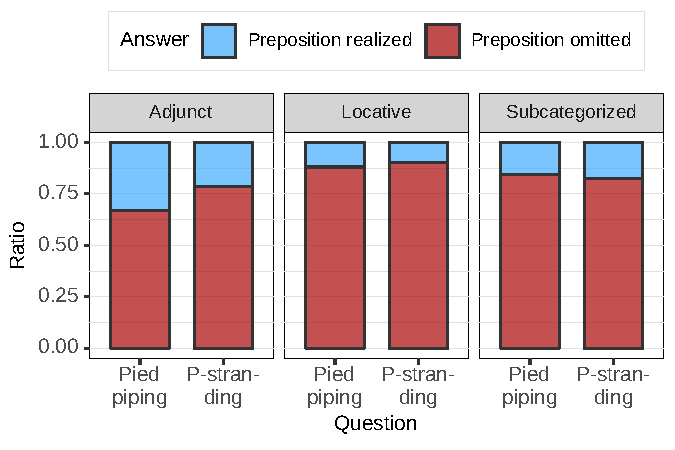
\includegraphics[scale=1]{figures/ex8_prod_relfrag_answers}
 \caption{Ratio of preposition omission/realization across conditions\label{fig:ex8_prod_fragments}.}
\end{figure}

\textsc{PPType} was a ternary factor, therefore the data had to be analyzed by conducting pairwise comparisons between factor levels just like in experiment \ref{exp:pstranding-defaultcase}. A first analysis compared the two types of complement PPs\is{Preposition phrase}, i.e. locative and subcategorized PPs, which each other. The initial model contained main effects for \textsc{Question}, \textsc{PPType}, \textsc{Position} (numeric) and all two-way interactions between these predictors. The model had only random intercepts for subjects and items, because it did converge with a more complex random effects structure. As the difference between locative and subcategorized PPs\is{Preposition phrase} did not turn out to be significant \glmernonsig{0.57}{0.5}, these conditions were pooled for further analysis and hence compared only adjunct\is{Adjunct} to complement PPs\is{Preposition phrase}. 

After pooling locative and subcategorized PPs\is{Preposition phrase}, the complete data set could be analyzed at once. 
The initial model contained main effects for \textsc{Question}, \textsc{PPType} (now binary), \textsc{Position} and all two-way interactions between these predictors. The model had only random intercepts for subjects and items and a by-subject random slope for \textsc{PPType}, because it did not converge with a more complex random effects structure. The final model (see Table \ref{tab:pstranding-production-estimates}) contains significant effects for both IVs: The preposition in the short answer fragment\is{Fragment, short answer} is more likely to be omitted\is{Preposition omission} when the PP\is{Preposition phrase} is a complement than when it is an adjunct\is{Adjunct} \glmer{5.23}{0.05}. What is more important with respect to the goal of the experiment is that the preposition is also more likely to be omitted\is{Preposition omission} in the answer when it is stranded\is{Preposition stranding} in the question \glmer{4.85}{0.05}. There is no significant interaction between the IVs  \glmernonsig{0.86}{0.3}.

\begin{table}[t]
\begin{tabular}{l l l l l l}
\lsptoprule
Predictor & Estimate & SE & $\chi^2$ &  $p$-value &  \\   
\midrule
\textsc{Question} & 0.719 &  0.308 & 4.85 & \textless 0.05 & * \\
\textsc{PPType} & 1.822 &     0.727 &   5.23 &  \textless 0.05 & *\\
\lspbottomrule
\end{tabular}
\caption{Fixed effects in the final GLMM for experiment \ref{exp:pstranding-production}.\label{tab:pstranding-production-estimates}}
\end{table}

\subsubsection{Discussion}
Experiment \ref{exp:pstranding-production} had the purpose of testing the nonsyntactic explanation for the crosslinguistic coincidence between the availability of preposition omission\is{Preposition omission} in short answers\is{Fragment, short answer} and of P-stranding\is{Preposition stranding} in questions: Speakers tend to match the form of the answer with that of the question, therefore, if a language has no P-stranding\is{Preposition stranding} in questions, preposition omission\is{Preposition omission} in the answer will be degraded. The experiment supports this hypothesis: If the preposition is stranded\is{Preposition stranding} in the question it is significantly more likely to be omitted\is{Preposition omission} than when it is pied-piped\is{Pied-piping}. This is the result that question-answer parallelism predicts.

In absolute terms, the effect seems to be less pronounced than the one found by \citet{nykiel2017} in her corpus study\is{Corpus}. This could be in part due to the restriction to P-stranding\is{Preposition stranding} and pied-piping\is{Pied-piping} questions as antecedents, whereas \citet{nykiel2017} investigated a larger variety of antecedents and remnants. Furthermore, the experimental design might have contributed to reducing the effect of the antecedent. First, although they were not told to do so, a few participants noted that some of the questions were not totally natural by adding a comment like ``the question sounds odd'' in the text field.%
%
\footnote{These responses were not analyzed.}\afterfn%
%
As I discussed above, P-stranding\is{Preposition stranding} is preferred in colloquial speech (recall that the experimental stimuli were presented as informal dialogues) for complement PPs\is{Preposition phrase} and dispreferred for adjunct\is{Adjunct} PPs\is{Preposition phrase}. Therefore, in each condition one of the questions is not perfectly natural, and in natural settings there is probably a higher ratio of P-stranding\is{Preposition stranding} in questions for complement than for adjunct\is{Adjunct} PPs\is{Preposition phrase}. Since the form of the question affects that of the answer, in corpus\is{Corpus} data this would probably increase the difference in counts of each of the answer variants as compared to the more controlled setting of the experiment. Second, even though the \textsc{Position} effect is not significant, subjects produced a relatively large amount of answers throughout the experiment and probably got used to the task and matched their answers to a lesser degree to the form of the question due to familiarization. This is tentatively supported by the observation that parallelism is most pronounced for the first item that each subject saw: Subjects who saw a complement PP in the question almost always omitted the preposition\is{Preposition omission} in the answer (90\% omission rate for pied-piping\is{Pied-piping} and 90.9\% for P-stranding\is{Preposition stranding}), but only 16.7\% of those who saw a pied-piped\is{Pied-piping} adjunct\is{Adjunct} PP in the question and all of those who saw a P-stranded\is{Preposition stranding} one did so. These numbers are not significant due to the reduced number of observations, but they suggest that a crowdsourced experiment with only one trial per subject might be a promising option to prevent such a familiarization effect.

\largerpage
The preference for preposition omission\is{Preposition omission} in all conditions is in line with the English\is{English} corpus\is{Corpus} data in \citet{nykiel2017}. She also reports that the preposition is omitted\is{Preposition omission} more often than it is realized both when it is pied-piped\is{Pied-piping} and stranded\is{Preposition stranding} in the antecedent. This overall preference for preposition omission\is{Preposition omission} is unexpected under the structured propositions account of question-answer parallelism. If pied-piping\is{Pied-piping} occurs because the preposition belongs to the focus of the question, and the focus structure of the answer is determined by that of the question, one would theoretically expect a perfect match between both. Such an effect can be reduced in experimental settings, but pied-piping\is{Pied-piping} in the question does not result in an inversion of participants' preferences in any of the conditions. The data are therefore tentatively more in line with the structural persistence account. From a processing\is{Processing effort} perspective, competing constraints introduce a probabilistic bias that can be overridden by others. Speakers might tend to omit the preposition\is{Preposition omission} because it is given, and this constraint might cancel out part of the effect of the tendency to reuse material given in context. Furthermore, the effect of constraints that are specifically relevant for oral on-line communication might be less prominent in experimental settings.%
%
\footnote{See e.g. \citet{zhan.etal2017}, who did not find effects of audience design\is{Audience design} in a production study\is{Production task}, even though such effects had been attested in related previous work.}\afterfn
%
Recall also that the relative acceptability of proper noun DP\is{Determiner phrase} fragments as short answers\is{Fragment, short answer} to PP\is{Preposition phrase} questions \citep{lemkeaccepted} also suggests that some deviation from question-answer congruence is possible even in German\is{German}. This is unexpected under a semantic account.

\noindent The main effect of \textsc{PPType} is in line with the observation by \citet{vanriemsdijk1978} that P-stranding\is{Preposition stranding} is less acceptable in adjunct\is{Adjunct} than in complement PPs\is{Preposition phrase}. However, this tendency does not override the preference for omitting the preposition\is{Preposition omission} in the experiment: The ratio of omitted prepositions\is{Preposition omission} is indeed the lowest observed throughout the experiment if the PP is an adjunct\is{Adjunct} and the preposition pied-piped\is{Pied-piping} in the question (see Figure \ref{fig:ex8_prod_fragments}). Still, even in this case, 67\% of prepositions are omitted\is{Preposition omission}. This might suggest that the syntactic relationship between the preposition and the verb at least affects preposition omission\is{Preposition omission} in fragments.

Taken together, the production study\is{Production task} supports a nonsyntactic question-answer parallelism. If the form of short answers\is{Fragment, short answer} follows that of questions, the absence of P-stranding\is{Preposition stranding} in German\is{German} questions explains straightforwardly why DP\is{Determiner phrase} fragments are degraded in such contexts. The experiment does not allow for a conclusion on why we observe this parallelism, but the strong overall preference for omitting the preposition\is{Preposition omission} in the answer seems to be more in line with a processing\is{Processing effort} account than with the structured propositions approach. This finding does not falsify the movement and deletion\is{Movement and deletion account} account. Movement and deletion\is{Movement and deletion account} is neither incompatible with the assumption of differing focus structures between pied-piping\is{Pied-piping} and P-stranding\is{Preposition stranding} questions nor with structural persistence. However, both of these accounts explain the pattern observed for fragments without assuming movement as an obligatory step\is{Movement and deletion account} in the derivation of fragments. This clearly weakens the status of the PSG\is{P-Stranding Generalization} as genuine evidence for movement.

\subsection{General discussion: Preposition omission} \label{sec:pstranding-discussion}
In section \ref{sec:pstranding} I presented four experiments that tested the predictions of the PSG\is{P-Stranding Generalization}, which is taken to be one of the central pieces of evidence for movement\is{Movement and deletion account} in fragments, and the viability of non-movement explanations for the data. Experiments \ref{exp:pstranding-german} and \ref{exp:pstranding-english} empirically support the predictions of the PSG\is{P-Stranding Generalization} for German\is{German}, where prepositions are obligatorily pied-piped\is{Pied-piping} in questions, and for English\is{English}, which allows for P-stranding\is{Preposition stranding}. Just like the PSG\is{P-Stranding Generalization} predicts, in German\is{German} there is a strong preference for realizing the preposition, whereas in English\is{English} its omission\is{Preposition omission} is acceptable, and actually preferred in the context of questions with P-stranding\is{Preposition stranding}.

A further result of experiment \ref{exp:pstranding-english} is that fronting the PP\is{Preposition phrase} in a complete sentence in English\is{English} is heavily degraded, as has been already noted by \citet{weir2014a}. This questions some of the arguments by \citet{merchant2004}, which are based on the idea that the acceptability of fragments patterns with that of left dislocation structures. The low ratings for both pied-piping\is{Pied-piping} and P-stranding\is{Preposition stranding} in the answer suggest that a movement and deletion\is{Movement and deletion account} account is viable only if exceptional movement\is{Exceptional movement account} is assumed, as \citet{weir2014} proposes. The exceptional movement\is{Exceptional movement account} account however requires an explanation for why the preposition is sometimes pied-piped\is{Pied-piping} in English\is{English}. If extraction out of the PP\is{Preposition phrase} is possible, and only the DP\is{Determiner phrase} complement of P is focused, there is no need to front the complete PP\is{Preposition phrase} in English\is{English}. For German\is{German} this is not a problem, because pied-piping\is{Pied-piping} is the only way to extract the focused DP\is{Determiner phrase} out of the ellipsis site if extraction out of PP\is{Preposition phrase} is blocked for independent reasons in this language.

Although the experiments \ref{exp:pstranding-german} and \ref{exp:pstranding-english} are in line with the PSG\is{P-Stranding Generalization}, they only provide evidence for movement\is{Movement and deletion account} if explanations under derivationally simpler accounts, such as the nonsentential\is{Nonsentential account} and \textit{in situ} deletion\is{In situ deletion account} accounts, must be ruled out. Experiments \ref{exp:pstranding-defaultcase} and \ref{exp:pstranding-production} tested two of these alternative explanations.

Experiment \ref{exp:pstranding-defaultcase} investigated the hypothesis that, as suggested by \citet{barton.progovac2005}, the preposition cannot be omitted\is{Preposition omission} in languages with strong case features\is{Case feature} because prepositional case\is{Prepositional case} is structural case\is{Structural case} and must always be checked. According to their theory, prepositional case\is{Prepositional case} cannot be checked in fragments because there is no unarticulated syntactic material that could do so (in this case, a preposition). Instead, they expect DPs\is{Determiner phrase} to appear in default case. The data clearly disconfirm this prediction: Default case\is{Default case} was rated\is{Acceptability rating task} even worse than the significantly degraded prepositional case\is{Prepositional case}-marked DPs\is{Determiner phrase}. Consequently, the case checking\is{Case feature} hypothesis, at least in the version suggested by \citet{barton.progovac2005}, must be discarded. Experiment \ref{exp:pstranding-defaultcase} also provides further evidence against the nonsentential account\is{Nonsentential account}, because presumably ungrammatical prepositional case\is{Prepositional case}-marked DP fragments are rated\is{Acceptability rating task} as more acceptable than grammatical, yet possibly pragmatically odd, nominative\is{Nominative case} DP fragments. Furthermore, the experiment questions the cleft\is{Cleft}-based analysis of preposition-less fragments in languages that lack P-stranding\is{Preposition stranding} \citep{szczegielniak2008, rodrigues.etal2009}. In German\is{German}, fragments derived from clefts\is{Cleft} must exhibit nominative\is{Nominative case} case morphology, but the experiment shows that nominative\is{Nominative case} DP fragments are degraded not only as compared to PPs\is{Preposition phrase} but also to presumably ungrammatical prepositional case\is{Prepositional case}-marked DP fragments.

Experiment \ref{exp:pstranding-production} addressed the hypothesis that the crosslinguistic variation found in fragments is the result of a tendency for answers to structurally match the corresponding questions. I discussed two possible explanations for this, one in terms of a structured propositions account of question semantics \citep{reich2002, griffiths2019} and one based on a tendency to reuse syntactic structure from previous discourse \citep{levelt.kelter1982}. Question-answer parallelism provides a straightforward account of the P-Stranding Generalization\is{P-Stranding Generalization}: If the preposition is pied-piped\is{Pied-piping} in the question, it is necessarily, or at least preferably, realized in the answer. Since the preposition is always pied-piped\is{Pied-piping} in languages like German\is{German}, it is never omitted\is{Preposition omission} in short answers\is{Fragment, short answer}. For languages that allow for both pied-piping\is{Pied-piping} and P-stranding\is{Preposition stranding}, the form of an answer would tend to match that of the question: Pied-piping\is{Pied-piping} in the question would yield a relatively higher ratio of PP\is{Preposition phrase} short answers\is{Fragment, short answer}, and P-stranding\is{Preposition stranding} more DP\is{Determiner phrase} short answers\is{Fragment, short answer}. Experiment \ref{exp:pstranding-production} provides evidence for such a preference using a production task\is{Production task}. The experiment could hence replicate the effect observed in a corpus study\is{Corpus} by \citet{nykiel2017} and the evidence for structural parallelism by \citet{levelt.kelter1982} in a controlled experiment that investigated specifically effects of P-stranding\is{Preposition stranding}/pied-piping\is{Pied-piping} in question on the form of the answer. However, despite a significant effect of the question's form, preposition omission\is{Preposition omission} was preferred in all conditions in absolute terms. The parallelism between question and answer seems to be weaker than expected under a structured propositions account, hence an explanation in terms of structural persistence tentatively seems to fit the observed pattern better.

The evidence for question-answer parallelism does not contradict the movement and deletion\is{Movement and deletion account} account, because syntactic theories do not neglect effects of processing\is{Processing effort} constraints but restrict the set of alternative expressions on which such constraints operate. However, experiment \ref{exp:pstranding-production} evidences that the form of the question affects the form of the answer in English\is{English}. If it does so in German\is{German} too, this provides a straightforward non-movement explanation for the preposition omission\is{Preposition omission} data: DP\is{Determiner phrase} short answers\is{Fragment, short answer} are not degraded in German\is{German} because they are ungrammatical, but because they never match the form of the question. As I argued above, it depends on the viability of non-movement accounts of the preposition omission\is{Preposition omission} data whether they constitute evidence for movement or not. The parallelism between question and answer evidenced in my experiment and in \citet{nykiel2017} provides such an explanation and consequently undermines the status of the preposition omission\is{Preposition omission} data as evidence for movement\is{Movement and deletion account}.

Taken together, preposition stranding\is{Preposition stranding} does not uniquely support the movement and deletion\is{Movement and deletion account} account as strongly as claimed by \citet{merchant2004}. Specifically, the data can be equally well explained in terms of question-answer parallelism under the assumption of and \textit{in situ} deletion\is{In situ deletion account} account. The nonsentential account\is{Nonsentential account} is of course also compatible with processing constraints\is{Processing effort}, however it predicts that prepositions cannot be omitted\is{Preposition omission} if the DP\is{Determiner phrase} is case-marked. This has been disconfirmed by experiment \ref{exp:pstranding-defaultcase}. In the next section I investigate a further movement restriction\is{Movement restriction} on complement clause\is{Complement clause} topicalization, which has been argued to hold crosslinguistically in Germanic languages \citep{webelhuth1992} and that has already been empirically investigated by \citet{merchant.etal2013}.


\section{Movement restrictions: Complementizer omission}
\label{sec:ccs}

\subsection{Complementizer omission as evidence for movement}\label{sec:ccs-background}
\subsubsection{Movement restrictions on complement clauses}
The second movement restriction\is{Movement restriction} that I investigate empirically is the (im)possibi\-lity of fronting complementizer-less\is{Complementizer omission} complement clauses\is{Complement clause} (in what follows, CCs\is{Complement clause}).%
%
\footnote{\citet[83--85]{webelhuth1992} argues that a similar pattern holds across all Germanic languages, the difference being that some do not allow for complementizer omission\is{Complementizer omission} \textit{in situ}.} %
%
This restriction is particularly relevant to the movement and deletion\is{Movement and deletion account} account because \citet{merchant2004} argues that it constrains the form of fragments and \citet{merchant.etal2013} present empirical evidence in support of this prediction.

According to \citet{merchant2004}, it was \citet{stowell1981} who first noted that only CCs\is{Complement clause} headed by an overt complementizer can appear in a sentence-initial position.%
%
\footnote{\citet{stowell1981} in turn attributes the observation to \citet{kayne1981}, but \citet[744]{morgan1973} makes a similar point even before that.}\afterfn%
%
\citet[396f]{stowell1981} observes that this holds for both subject CCs\is{Complement clause} \Next[a] and topicalized object CCs\is{Complement clause} \Next[b]. \Next[c] shows that omitting the complementizer\is{Complementizer omission} in object position is possible, hence the ungrammaticality must be attributed to the sentence-initial position of the CC.%
%
\footnote{
\citet[396]{stowell1981} explains the data by arguing that complementizer-less CCs\is{Complement clause} are headed by a phonetically null element, which c-commanded by the verb according to the Empty Category Principle \citep{chomsky1981}. This is possible only in the complement position, but not when the clause is base-generated in the subject position \Last[a] or moved to the topic position \Last[b].}\afterfn%
%

\ex. \a. *(That) the teacher was lying was hardly obvious.
      \b. *(That) the teacher was lying, Ben already knew.
 \c. Ben knew the teacher was lying.

\citet{merchant2004} cites \citet{morgan1973} with the observation that the same restriction holds for CP\is{Complementizer phrase} fragments, under the condition that the speaker ``does not believe or subscribe to [the meaning of the fragment, R.L.]'' \citep[690]{merchant2004}, i.e. when it is non-factive\is{Factivity} \Next[a]. The contrast between \Next[b] and \Next[c] shows that the complementizer is obligatory only when the CC\is{Complement clause} is topicalized \Next[c], but that it can be omitted\is{Complementizer omission} when the CC\is{Complement clause} remains \textit{in situ}. 

\ex.
\a. What does no one believe? \hfill \citep[690]{merchant2004}\\
\mbox{}\hspace{-.45em}\#(That) I’m taller than I really am.
\b. No one believes (that) I'm taller than I really am. \label{ex:merchant-cc-insitu}
\c. *(That) I’m taller than I really am, no one believes. \label{ex:merchant-cc-fronted}

\citeauthor{merchant2004} argues that this challenges \textit{in situ} deletion accounts\is{In situ deletion account} of fragments, which must explain why the complementizer cannot be omitted\is{Complementizer omission} in fragments even though this is possible in full sentences when the CC\is{Complement clause} appears \textit{in situ}.

Taken together, according to the literature the pattern seems to be robust for non-factive\is{Factivity} CCs\is{Complement clause} of verbs: Only CCs\is{Complement clause} with overt complementizers may be fronted. If the derivation of fragments involves regular A'-movement, as \citet{merchant2004} claims, this predicts fragment CCs\is{Complement clause} to always require overt complementizers. As I repeatedly noted above, if exceptional movement\is{Exceptional movement account} is assumed, it is crucial to determine whether this movement is available ``in principle'' or not, but \citet{weir2014} does not provide criteria that determine whether this is true for a specific movement operation. Since the literature on the phenomenon cites no acceptable instance of this beyond parenthetical uses,%
\footnote{\citet{webelhuth1992} argues that the following example is fine, provided an intonational break after the first clause:

\exg. [Hans ist krank gewesen] hat Peter gemeint.\\
Hans is sick been has Peter meant\\
\trans{Peter thought Hans had been sick.} \exsourceraised{\citep[89]{webelhuth1992}}

}\afterfn%
%
it is probably to be classified as not available in principle. Non-movement accounts in turn require an independent explanation for why the complementizer cannot be omitted\is{Complementizer omission}. However, the pattern is currently only partially empirically supported. Therefore, before any conclusions can be drawn it must be empirically investigated whether it actually holds. This is the goal of the experiments in Section \ref{sec:ccs}. 

\subsubsection{Previous experimental evidence}
\citet{merchant.etal2013} present first experimental evidence for an apparent parallelism between the movement restriction\is{Movement restriction} on complementizer-less\is{Complementizer omission} CCs\is{Complement clause} and the form of fragments. In their experiment 1, they tested short answer fragments\is{Fragment, short answer} like \Last[a] in an acceptability rating\is{Acceptability rating task} study. They find that fragments headed by an overt complementizer ($\mu$ = 4.25 on a 5-point scale, where 5 = perfect) are rated\is{Acceptability rating task} significantly better than complemen\-tizer-less ones ($\mu$  = 3.73) and interpret this as reflecting a movement restriction\is{Movement restriction} on comple\-mentizer-less CCs\is{Complement clause}. Since movement and deletion\is{Movement and deletion account} predicts that complementizer omission\is{Complementizer omission} is ungrammatical, the ratings for these fragments are surprisingly high. \citet{merchant.etal2013} suggest that this is due to the possibility of interpreting complementizer-less\is{Complementizer omission} CCs\is{Complement clause} as indirect answers. With an indirect answer, the speaker does not give a congruent answer to the question (as discussed in Section \ref{sec:theories-insitu}), but provides any piece of information that might help his interlocutor to figure out an answer. For instance, in \Next Mary does not commit herself to the claim that the defeat is the reason for John being angry, but she suspects that the defeat might be the reason for John's anger.

\ex. Bill: Why is John so angry?\\
    Mary: (I'm not sure, but) Barcelona lost to Liverpool yesterday.
    
The study by \citet{merchant.etal2013} leaves open several issues: (i) Acceptability ratings\is{Acceptability rating task} were collected only for fragments,  (ii) some items include CCs\is{Complement clause} of prepositions, (iii) some of the matrix verbs are factive\is{Factivity}, and (iv) they do not explore alternative explanations that do not imply movement for the data. In what follows I review these issues in greater detail.

First, \citet{merchant.etal2013} tested the acceptability\is{Acceptability rating task} of fragment CCs\is{Complement clause} but not of corresponding topicalization structures. The authors assume that the introspective contrast between \ref{ex:merchant-cc-insitu} and \ref{ex:merchant-cc-fronted}, which has been repeatedly cited in the literature since \citet{stowell1981}, accounts for the measured acceptability of the corresponding fragments. However, some native speakers of American English\is{English} that I consulted do not share the grammaticality judgments that \citet{merchant.etal2013} assign to the topicalized CCs\is{Complement clause}. Furthermore, \citet{featherston2007} notes that introspective data sometimes do not generalize to a larger population and withstand empirical investigation despite of being widely agreed on and repeatedly cited in the theoretical literature. The validity of the pattern in \LLast however is crucial to the experiment by \citet{merchant.etal2013}: If it was not confirmed, the judgments for fragments could not be attributed to those for the presumably underlying left dislocation structures. This calls for an empirical investigation of both the fragments and corresponding left dislocation structures.

Second, half ($n$~=~8) of the items tested by \citet{merchant.etal2013} involve CCs\is{Complement clause} which are embedded under a PP\is{Preposition phrase}, like \Next. These CCs\is{Complement clause} are always ungrammatical \textit{in situ} \Next[a], whereas they are acceptable when the complementizer is present in a fronted position \Next[b] and as a fragment \Next[c]. Even though \citet{merchant2004} argues that this speaks against the \textit{in situ} deletion\is{In situ deletion account} account, actually it does not: \textit{In situ} deletion\is{In situ deletion account} takes regular grammatical sentences as the input for ellipsis and analyzes ellipsis as a post-spellout phenomenon. If movement of the CC\is{Complement clause} is obligatory for whatever reason, it has to occur before ellipsis, so that the only grammatical input for \textit{in situ} deletion\is{In situ deletion account} is \Next[b] with an overt complementizer.

\ex. What are you ashamed of?
\a. *I am ashamed of (that) I ignored you.
\b. *(That) I ignored you, I am ashamed of.
\c. *(That) I ignored you.

\is{Factivity|(}Third, among the remaining eight items, some contained factive\is{Factivity} matrix verbs, like \textit{to regret} in \Next. Factive\is{Factivity} verbs, which presuppose the truth of their complement, as \textit{to regret} or \textit{to conceal} do, are widely assumed to require, or at least strongly prefer, CCs\is{Complement clause} with overt complementizers (see \citenob{kiparsky.kiparsky1970}; \citenob{hegarty1992}). \citet[689]{merchant2004} himself cites a related observation by \citet{morgan1973} that complementizers may not be omitted\is{Complementizer omission} when the speaker ``does not believe or subscribe'' to the content of the CC. Consequently, if the verb disprefers or even disallows complementizer-less\is{Complementizer omission} CCs\is{Complement clause} in general, any structure derived from it will be degraded, independently of whether the CC\is{Complement clause} is moved to the left periphery or whether the matrix clause is PF-deleted in situ.\is{Factivity|)}

\ex. What did John regret? \hfill \citep[31]{merchant.etal2013}\\
(That) he joined the Navy.

Finally, there are potential non-movement explanations for both the empirically observed fragment data and the introspective judgments on topicalization. As for fragments, a complementizer-less\is{Complementizer omission} answer can be interpreted both as a direct and as an indirect answer to a question, whereas a complementizer unambiguously marks the answer as direct. 
Therefore, the ratings reported by \citet{merchant.etal2013} possibly do not reflect grammaticality, but usage preferences. 
In what refers to complementizer omission\is{Complementizer omission} in full sentences, realizing the complementizer in fronted clauses could facilitate processing. When the hearer parses\is{Parser, human} a complementizer-less\is{Complementizer omission} CC, the complement clause\is{Complement clause} can be incorrectly analyzed as a matrix clause until the matrix verb is encountered. In contrast, the initial complementizer requires that the CC\is{Complement clause} is parsed\is{Parser, human} as the complement of a verb, and this will facilitate processing. This is also in line with corpus\is{Corpus} data by \cite{jaeger2010}, who shows that the likelihood of a CC\is{Complement clause} in a specific context predicts whether the complementizer will be omitted\is{Complementizer omission} or not.%
%
\footnote{The possibility of a processing account has already been discussed by \citet[397]{stowell1981}, who argues against the processing account based on data as \Next. The argument is that the CC\is{Complement clause} is very likely at the point where it occurs due to the subcategorization preferences of the predicate, and still the complementizer cannot be omitted\is{Complementizer omission}.

\ex. It surprises me *(that) you have heard about Roger.  \hfill \citet[397]{stowell1981}

}\afterfn%
%

\noindent In Section \ref{sec:ccs} I present experiments based on the study on complement clauses\is{Complement clause} by \citet{merchant.etal2013} in German\is{German} and English\is{English} (experiments \ref{exp:ccs-german} and \ref{exp:ccs-english}), which address these issues. In the I collect ratings for both topicalized and fragment CCs\is{Complement clause}, test only CCs\is{Complement clause} that are acceptable \textit{in situ} and use only non-factive\is{Factivity} matrix verbs. The goal of the experiments is two-fold. First, the data for fragment answers will show whether the preference for realizing the complementizer in fragments is replicated when controlling for factivity\is{Factivity}. Second, the data for left dislocation answers might provide empirical evidence for the movement restriction\is{Movement restriction} on complementizer-less\is{Complementizer omission} CCs\is{Complement clause} on which the experiment by \citet{merchant.etal2013} is based. Anticipating the results, the experiments suggest that the effect reported by \citet{merchant.etal2013} does not evidences a movement restriction\is{Movement restriction} on complementizer-less\is{Complementizer omission} CCs\is{Complement clause} but results from independent factors. The German\is{German} data replicate the preference for realizing the complementizer in fragments, but this effect is not reflected in the acceptability of the corresponding left dislocation structures. In English\is{English}, there is no significant difference between fragments at all and null complementizers are even preferred in full sentences.

\refstepcounter{expcounter}\label{exp:ccs-german}
\subsection{Experiment \ref{exp:ccs-german}: CC topicalization in German} 
\label{sec:ccs-german}

\subsubsection{Background}\label{sec:ccs-german-background}
Experiment \ref{exp:ccs-german} replicates experiment 1 in \citet{merchant.etal2013} in German\is{German} under more controlled conditions. As compared to the study by \citet{merchant.etal2013}, there were four main modifications: First, the experiment was conducted in German, second, I used a context story to preclude the possibility of an indirect answers interpretation, third, I tested both fragments and full sentences, and fourth, I added a third condition, subjunctive mood verb-second CCs\is{Complement clause}.

\noindent As for the first modification, in German I expected a similar pattern to the English data in \citet{merchant.etal2013}. \citet[83]{webelhuth1992} claims that subject CCs\is{Complement clause} require overt complementizers in all Germanic languages.%
%
\footnote{\citeauthor{webelhuth1992} presents \Next as evidence in favor of this claim. However, omitting the complementizer\is{Complementizer omission} in verb-last CCs\is{Complement clause} is also unacceptable \textit{in situ} and cannot be attributed to the prefield\is{Prefield} position \NNext[a]. In the case of the example, its verb-second counterpart \NNext[b] seems to be degraded as well. A further shortcoming of the example is that the predicate is factive\is{Factivity}, so that complementizer omission\is{Complementizer omission} seems to be dispreferred \textit{in situ} \NNext[c]. \NNext[c] is only acceptable with a break in intonation between the first and the second clause that marks that each clause is an independent sentence.

\exg. *(Da\ss) Hans nicht kommt, ist schade.\\
that Hans not comes is pity\\
\trans{It is a pity that Hans does not come.}\exsourceraised{\citep[83]{webelhuth1992}}

\ex. \ag. Es ist schade, *(dass) Hans nicht kommt.\\
	  it is pity that Hans not comes\\
     \bg. *Hans kommt nicht, ist schade.\\
	  Hans comes not is pity\\
    \cg.  *Es ist schade, Hans kommt nicht.\\
	  it is  pity Hans comes not\\
	  \trans{It is a pity (that) Hans does not come.}


}\afterfn %

The target sentence was introduced by a context story and a short dialogue with two turns per speaker \Next. The context story had the purpose of making an indirect answer less likely. \citet{merchant.etal2013} suggest that complementizer-less\is{Complementizer omission} CCs\is{Complement clause} were rated\is{Acceptability rating task} as relatively acceptable\is{Acceptability rating task} in their experiment due to their interpretation as indirect answers. In my experiment, the context stories ensured that this was not possible: For instance, in \Next, it is very unlikely that the reporter has sufficient knowledge about the crime to give an indirect answer. The CCs\is{Complement clause} were tested not only as fragments, but also in a left-peripheral position within a complete sentence in order to investigate whether the assumed movement restriction\is{Movement restriction} on complementizer-less\is{Complementizer omission} CCs\is{Complement clause} is empirically confirmed. Furthermore, acceptability differences between the sentential conditions allow me to test the prediction of the movement and deletion\is{Movement and deletion account} account that the acceptability of left dislocations matches that of the corresponding fragments.

Finally, besides the German\is{German} counterparts of the CCs\is{Complement clause} investigated by \citet{merchant.etal2013}, I added a third type of complement clause\is{Complement clause}, verb-second complement clause\is{Complement clause}s in subjunctive mood, to test the hypothesis that verb-second CCs\is{Complement clause} are rated\is{Acceptability rating task} as acceptable because they are interpreted as indirect answers.

\newpage
\ex. [Context story] This weekend a famous painting has been stolen from the museum. The newscaster is reporting on the investigation of the robbery.\\ \mbox{}[Newscaster:] What's the news about the art robbery?\\ \mbox{}[Reporter:] The investigators are discussing how the burglar got into the building.\label{ex:ccs-experiment-sample-item}
\ag. [N:] Was glaubt Kommissar Wagner?\\
\mbox{} what believes inspector Wagner\\
\trans{[N:] What does inspector Wagner believe?}
\bg. [R:] Dass der Täter durch  das Fenster  eingestiegen ist.\\
     \mbox{} that  the thief through the window  entered is\\
     \trans{[R:] That the thief entered through the window.}

The reason for this is that CCs\is{Complement clause} headed by \textit{dass}, the German\is{German} equivalent to \textit{that}, are verb-last, whereas complementizer-less\is{Complementizer omission} CCs\is{Complement clause} are always verb-second. Therefore, verb-second complement clause\is{Complement clause}s are ambiguous between a direct answer (a CC\is{Complement clause} fragment) and an indirect answer (a matrix clause). Since subjunctive mood encodes reported speech in German\is{German}, it enforces the interpretation as a direct answer. If indicative complementizer-less\is{Complementizer omission} CCs\is{Complement clause} were rated\is{Acceptability rating task} as more acceptable only because they can be interpreted as indirect answers, they would be more acceptable than subjunctive ones. Subjunctive might also provide some insights on the viability of the pragmatic and processing accounts of complementizer omission\is{Complementizer omission} that I sketched above. If complementizer-less\is{Complementizer omission} fragments are dispreferred due to their ambiguity\is{Ambiguity}, subjunctive should improve their acceptability because it excludes the possibility of an indirect answer. Similarly, in fronted CCs\is{Complement clause} the likelihood of an embedding matrix verb will increase as soon as the inflected verb in the CC\is{Complement clause} is encountered. Since the CC\is{Complement clause} is verb-second, this happens relatively early, hence processing\is{Processing effort} it should be easier in comparison to the indicative verb second clause. This setting yields a 2$\times$3 design that crosses \textsc{Sententiality} and \textsc{CCType}.\largerpage

The movement and deletion\is{Movement and deletion account} account predicts that, if complementizer-less\is{Complementizer omission} CCs\is{Complement clause} are degraded as full sentences, they will be as fragments, too. If the movement restriction\is{Movement restriction} on complementizer-less\is{Complementizer omission} CCs\is{Complement clause} was not empirically supported, \citet{merchant2004} predicts that whatever pattern is observed, there should be no interaction between \textsc{Sententiality} and \textsc{CCType}. The \textit{in situ} deletion\is{In situ deletion account} account makes no specific predictions with respect to this, because it does not assume that left dislocation structures are the input to the derivation of fragments. \textit{In situ} deletion\is{In situ deletion account} might predict a parallelism between the acceptability of complement clauses\is{Complement clause} as fragments and in their base position, but if both the realization and the omission of the complementizer is grammatical for non-factive\is{Factivity} matrix verbs it is unlikely that this results in a strong acceptability contrast.

\subsubsection{Materials}\label{sec:ccs-materials}
All materials follow the pattern in \Last. The target utterance is preceded by a two-sentence context story and a dialogue between two characters. The context story is always such that the character who produces the target utterance is not in the epistemic position to produce an indirect answer. The target utterance is the second turn by the second character. In the sentential conditions, the matrix clause in the target utterance (\textit{glaubt er}, `he believes') is given in the immediately preceding question. Table \ref{tab:ccs-german-materials} provides an overview of the conditions for the target sentence in \Last.

\begin{table}[t]
 \begin{tabular}{l l l}
 \lsptoprule
  Target utterance & Condition\\
\midrule
Dass der Täter durch  das Fenster  eingestiegen ist, glaubt er. &VL, sent.\\
Der Täter ist durch das Fenster  eingestiegen, glaubt er. & V2, ind, sent.\\
Der Täter sei durch das Fenster  eingestiegen, glaubt er. & V2, ind, sent.\\
Dass der Täter durch  das Fenster  eingestiegen ist. &VL, frag.\\
Der Täter ist durch das Fenster  eingestiegen. & V2, ind, frag.\\
Der Täter sei durch das Fenster  eingestiegen. & V2, ind, frag.\\

  \lspbottomrule
 \end{tabular}
\caption{Target sentences in experiment \ref{exp:ccs-german}. See example \ref{ex:ccs-experiment-sample-item} for glosses. The subjunctive  is distinguished from indicative only by the copula (\textit{sei} instead of \textit{ist}).\label{tab:ccs-german-materials}}
\end{table}

The issue that factive verbs\is{Factivity} prefer CCs\is{Complement clause} with overt complementizers according to the literature \citep{kiparsky.kiparsky1970, hegarty1992} was addressed by testing only three non-factive\is{Factivity} matrix verbs (\textit{glauben} `to believe’, \textit{meinen} `to mean' and \textit{sagen} `to say'). A corpus\is{Corpus} search on the German\is{German} newspaper corpus\is{Corpus} TüBa-D/Z \citep{telljohann.etal2004} confirms that each of the three verbs occurs with each of the CC\is{Complement clause} types investigated, but they seem to differ quantitatively in their subcategorization preferences, as Table \ref{tab:ccs-matrixv-frequency} shows. In order to factor out possible subcategorization preferences of specific verbs I included the \textsc{MatrixVerb} as a predictor in the statistical analysis. However, the analysis showed that the verb has no significant effect on acceptability.

\begin{table}[t]
 \begin{tabular}{l r l l}
 \lsptoprule
  verb & VL CC\is{Complement clause} & V2 indicative CC\is{Complement clause} & V2 subjunctive CC\is{Complement clause}\\
\midrule
  glauben & 50 (0.49) & 37 (0.36) & 15 (0.15)\\   
  sagen & 32 (0.27) & 34 (0.28) & 54 (0.45)\\  
  meinen & 8 (0.11) & 10 (0.14) & 52 (0.74)\\  
  \lspbottomrule
 \end{tabular}
\caption{Counts (ratio) in TüBa-D/Z of each type of CC for the three matrix verbs tested in experiment \ref{exp:ccs-german}.
\label{tab:ccs-matrixv-frequency}}
\end{table}
%
\subsubsection{Procedure}\label{sec:ccs-german-method}
The experiment was completed by 38 undergraduate students of Saarland University who were rewarded with the participation in a lottery of 10~$\times$~\currencyEuro{30.00}. All of them were native speakers of German\is{German}. The experiment was conducted over the Internet using the LimeSurvey presentation software. Subjects were asked to rate the naturalness of the critical utterance, which was italicized, in the context of the previous discourse on a 7-point Likert scale with labeled extremes (7 = totally natural). Subjects were assigned to one of six lists. As the topicalization structures are probably highly marked due to the redundant matrix clause and the heavy CC\is{Complement clause} in the initial position, that is dispreferred for processing reasons \citep{hawkins2004}, \textsc{Sententiality} was tested as a between subjects IV. Half of the subjects saw only topicalized CC\is{Complement clause}s and the other half only the corresponding fragments. Each subject thus rated\is{Acceptability rating task} 21 items (7 per \textsc{CCType} condition), which were mixed with 24 items from an unrelated experiment and 40 fillers. The materials were presented in individually fully randomized order. The fillers and items of the unrelated experiment had a similar structure as those of the current experiment. Subjects always rated\is{Acceptability rating task} an italicized target utterance that appeared at the end of a shot dialogue which was preceded by a context story. Three subjects who rated\is{Acceptability rating task} more than two out of five ungrammatical controls as acceptable (6 or 7 points on the scale) were excluded from further analyses.

\subsubsection{Results}\label{sec:ccs-german-results}

Figure \ref{fig:ccs-german-estimates} shows the averaged ratings across conditions. Fragments \descriptives{5.85}{1.54} were overall rated\is{Acceptability rating task} as better than sentences \descriptives{4.77}{1.75}.  Recall that \textsc{Sententiality} was tested between subjects, so that these figures cannot be directly compared to each other. Rather, they show that a floor effect for the topicalization conditions could be avoided by the between subjects design. Ratings for the verb-second conditions were very close to each other both within sentences ($\mu_{indicative} = 4.86$, $\mu_{subjunctive} = 4.9$) and fragments ($\mu_{indicative} = 5.72$, $\mu_{subjunctive} = 5.64$). Verb-last CCs\is{Complement clause} were rated\is{Acceptability rating task} slightly better than verb-second CCs\is{Complement clause} in the fragment \descriptives{6.21}{1.23} and slightly worse in the sentence condition \descriptives{4.56}{1.76}. 

\begin{figure}[t]
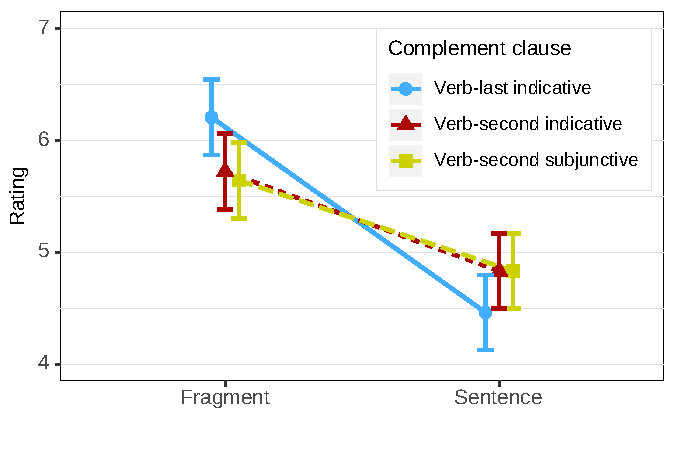
\includegraphics[scale=1]{figures/ex2b_ccs_de_lc_estimates}
 \caption{Mean ratings and 95\% confidence intervals across conditions in experiment \ref{exp:ccs-german}. \label{fig:ccs-german-estimates}}
\end{figure}
%
\noindent The data were statistically analyzed with CLMMs in \texttt{R} following the procedure described in Section \ref{sec:intro-stats}. Since \textsc{CCType} was a ternary factor, I first conducted an analysis on the data for verb-second CC\is{Complement clause}s only in order to test the conjecture that they did not differ significantly from each other. If this was confirmed, the two verb-second conditions could be pooled for further analysis and \textsc{CCType} treated as a binary predictor. The initial model for this analysis contained fixed effects for \textsc{CCType}, \textsc{Sententiality}, \textsc{Position} of the trial in the experiment and \textsc{MatrixVerb} in order to account for an effect of the verb's subcategorization preferences, as would be evidenced by a \textsc{MatrixVerb:CC\is{Complement clause}Type} interaction. As for random effects, I included by-subject and by-item random intercepts and random slopes for \textsc{Sententiality}, \textsc{MatrixVerb}, \textsc{CCType} and the interactions thereof.%
% 
\footnote{A by-subject random slope for \textsc{Sententiality} and the corresponding interactions were omitted as it would make no sense for a between subjects IV. Similarly, there was no by-item slope for \textsc{MatrixVerb} and interactions thereof, because \textsc{MatrixVerb} was not varied between items.}\afterfn%
%
Since the analysis of verb-second CCs\is{Complement clause} revealed no significant difference between subjunctive and indicative \clmmLRnonsig{0.19}{0.6} verb-second CCs, the verb-second conditions were pooled for further analysis. The full model fitted to the complete data set after pooling had the same effects structure as the model for verb-second CCs\is{Complement clause}.
\newpage

The final model is summarized in Table \ref{tab:ccs-german-estimates}. It contained significant main effects of both IVs and a significant interaction between them. The main effect of \textsc{Sententiality} \clmmLR{14.57}{0.001} confirms that fragments are rated\is{Acceptability rating task} better than left dislocations averaging over \textsc{CCType} conditions.%
%
\footnote{The significance of main effects of predictors that significantly interacted with others was assessed by the procedure described in \citet{levy2018}. I sum-coded the other predictor participating in the interaction and then compared a model that contains the predictor to be tested to one that does not with a likelihood ratio test.}\afterfn%
%
The main effect of \textsc{CCType} \clmmLR{6.02}{0.05} indicates that verb-last clauses were preferred over verb-second ones, and the significant \textsc{Sententiality:CC\is{Complement clause}Type} \clmmLR{25.75}{\highsig} interaction shows that this preference is specifically large for fragments. 
The \textsc{MatrixVerb} had no significant effect on acceptability and neither participated in any significant interaction. The significant main effect of \textsc{Position} \clmmLR{16.76}{\highsig} shows that items were perceived as more acceptable the later they appeared in the experiment, while the interaction with \textsc{Sententiality} \clmmLR{12.73}{0.001} suggests that this effect was stronger for fragments than for left dislocations. These predictors are not theoretically interesting, but their inclusion factors out the familiarization effects. 

\begin{table}[t]
\begin{tabular}{l l l l l l}
\lsptoprule
Predictor & Estimate & SE & $\chi^2$ &  $p$-value &  \\   
\midrule
\textsc{Sententiality}  & \phantom{-}0.834 &  0.231 &  14.57  &\textless 0.001 & ***\\
\textsc{CCType} & -0.19 &  0.067 & \phantom{1}6.02 &\textless 0.05 &* \\
\textsc{Position}   &   \phantom{-}0.009 &  0.002 &  16.76 & \textless \highsig & ***\\
\textsc{Sententiality:CC\is{Complement clause}Type} & -0.447 &  0.068 & 25.75 & \textless \highsig & ***\\
\textsc{Sententiality:Position}  &   \phantom{-}0.008 &  0.002 &  12.73 & \textless 0.001 & ***\\
\lspbottomrule
\end{tabular}
\caption{Fixed effects in the final CLMM for experiment \ref{exp:ccs-german}. \label{tab:ccs-german-estimates}}
\end{table}

In addition to the analysis of the complete data set, I performed an analysis of the sentential left dislocation conditions only in order to test the movement restriction\is{Movement restriction} on complementizer-less\is{Complementizer omission} CCs\is{Complement clause}. The full model had the same effects structure like the one in the main analysis, with the obvious exception that all effects for \textsc{Sententiality} were removed. The final model contained only a significant main effect of \textsc{CCType} \clmmLR{10.68}{0.01} evidencing that clauses headed by a complementizer were rated\is{Acceptability rating task} as significantly worse than their complementizer-less\is{Complementizer omission} counterparts.

\subsubsection{Discussion}
Experiment \ref{exp:ccs-german} investigated (i) whether fronting complementizer-less\is{Complementizer omission} CCs\is{Complement clause} is degraded as compared to CCs\is{Complement clause} headed by overt complementizers, and (ii) whether this movement restriction\is{Movement restriction} is reflected in the acceptability of fragments. 

The significant \textsc{Sententiality:CCType} interaction shows that the preference for realizing the complementizer\is{Complementizer omission} is stronger for fragments than for left dislocated CC\is{Complement clause}s. The analysis of the sentential conditions only shows that the preference for realizing the complementizer is even inverted in full sentences: In contrast to the claim by \citet{webelhuth1992}, who argues that this movement restriction\is{Movement restriction} is a property of ``all finite declarative argument clauses in the Germanic languages'' \citep[83]{webelhuth1992}, omitting the complementizer\is{Complementizer omission} is preferred in the full sentence. At least for German\is{German}, this undermines the reasoning upon which the interpretation of the data in \citet{merchant.etal2013} is based, since there is no evidence for a movement restriction\is{Movement restriction} on complementizer-less\is{Complementizer omission} CC\is{Complement clause}s. Furthermore, the sentential conditions seem to be grammatical across the board, as their mean ratings (for all conditions $\mu > 4.5$) are clearly above those for ungrammatical controls ($\mu = 2.4$). 

The fragment data alone resemble the pattern reported by \citet{merchant.etal2013}: Fragment CCs\is{Complement clause} are more acceptable when they are introduced by a complementizer than when they are not. However, since there is no evidence for the movement restriction\is{Movement restriction} stated in the literature, this effect cannot be attributed to constraints on movement. Furthermore, all three fragment conditions seem to be relatively acceptable, and even the dispreferred complementizer-less\is{Complementizer omission} fragments were rated\is{Acceptability rating task} much better than ungrammatical controls ($\mu = 2.18$). Unlike in the experiment by \citet{merchant.etal2013}, the explanation that they were interpreted as indirect answers is ruled out by the context story. Furthermore, there was no significant difference at all between subjunctive and indicative mood, even though the indirect answer interpretation is only possible in the indicative conditions. Since subjunctive encodes reported speech,  it cannot be interpreted as an indirect answer and they would have been preferred over indicative ones if the indirect answer explanation for the relatively high ratings for complementizer-less\is{Complementizer omission} CCs\is{Complement clause} in \citet{merchant.etal2013} was correct.

Taken together, the data indicate that, at least in German\is{German}, the preference for realizing the complementizer in short answer fragments\is{Fragment, short answer} observed by \citet{merchant.etal2013}, which my experiment replicates, seems not to be caused by a movement restriction\is{Movement restriction} on complementizer-less\is{Complementizer omission} CCs\is{Complement clause}. If this finding is robust and generalizes to English\is{English}, it would question the reasoning behind the experiment by \citet{merchant.etal2013}: If the movement restriction\is{Movement restriction} in question does not hold, no conclusions with respect to this can be drawn from the acceptability of the corresponding fragments. Experiment \ref{exp:ccs-english} will replicate this study in English\is{English} to investigate whether the difference between the results in \citet{merchant.etal2013} and my German\is{German} data evidences a cross-linguistic difference or whether it must be attributed to properties of the experiment design.

\subsubsection{Follow-up study with shorter contexts}

\subsubsubsection{Background and materials}
The stimuli tested in experiment \ref{exp:ccs-german} were relatively long and complex as compared to those used by \citet{merchant.etal2013}. Instead of a question-answer pair, they consisted of a context story and two turns per character. This might have biased subjects to base their ratings rather on the naturalness of the target utterance in discourse than on its grammaticality alone. In order to address this concern, I conducted a follow-up experiment using similar materials, but slightly longer context stories and two-turn dialogues which consisted only of the critical question-answer pair \Next.

\ex. [Context story] This weekend a famous painting has been stolen from the museum. The newscaster is reporting on the investigation of the robbery. The investigators are currently discussing how the burglar got into the building.\\\mbox{}[Newscaster:] Was glaubt Kommissar Wagner?\\\mbox{}[Reporter:]  Der Täter ist durch das Fenster eingestiegen(, glaubt er).

\subsubsubsection{Method}
The experiment was presented on the Internet using Lime\-Survey. Originally, it was conducted in the same session as the production study\is{Production task} on case marking (experiment \ref{exp:case-production}), where subjects were asked to produce utterances referring to graphical stimuli. The experiment was completed by 38 undergraduate students of Saarland University, who were rewarded with the participation in a lottery of 5 $\times$ \currencyEuro{30.00} among all participants.%
%
\footnote{Due to a technical problem, two out of the six lists (which included 10 subjects) were assigned experimental materials in the incorrect conditions. The corresponding participants were replaced by subjects recruited on the \textit{clickworker} crowdsourcing platform. These subjects rated\is{Acceptability rating task} the correct materials, which were mixed with the stimuli from experiment \ref{exp:mvb} and the same fillers as in the original lists. Each subject on the replacement lists was paid \currencyEuro{3.00} for participating. Since the distribution issue does not concern the stimuli of experiment \ref{exp:mvb}, in the case of experiment \ref{exp:mvb} I report the original data.}\afterfn%
%
The task and assignment to lists was identical to experiment \ref{exp:ccs-german} and \textsc{Sententiality} was tested between subjects again. Each subject rated\is{Acceptability rating task} 21 items (7 per \textsc{CCType} condition). Materials were presented together with 35 items of experiment \ref{exp:mvb} and 25 unrelated fillers including four ungrammatical controls in individually pseudo-randomized order. Pseudo-randomization ensured that no two items of the same experiment followed each other. One participant rated\is{Acceptability rating task} 50\% or more of the ungrammatical attention checks as acceptable (6 or 7 points on the scale) and was therefore excluded from further analysis.

\subsubsubsection{Results}
Figure \ref{fig:ccs-german-short-estimates} shows the aggregated ratings across conditions. The pattern is similar to experiment \ref{exp:ccs-german}, despite the slightly different ratings in absolute terms, which might be due to the differing materials that were tested together with the items in experiments \ref{exp:ccs-german} and the follow-up study.
%
\begin{figure}[t]
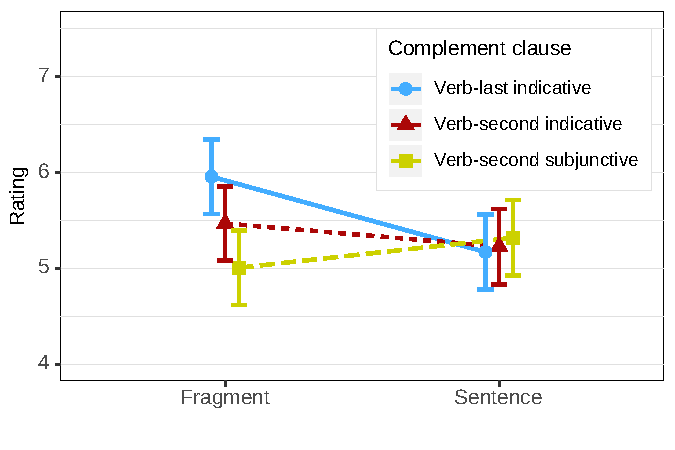
\includegraphics[scale=1]{figures/ex2b_ccs_de_sc_estimates}
 \caption{Mean ratings and 95\% confidence intervals across conditions in the follow-up to experiment \ref{exp:ccs-german}. \label{fig:ccs-german-short-estimates}}
\end{figure}
%
The statistical analysis followed the same procedure as for experiment \ref{exp:ccs-german}. First, pairwise analyses compared two of the three levels of \textsc{CCType} at a time. In all three analyses there were significant effects of \textsc{CCType} or significant interactions of \textsc{CCType} and \textsc{Sententiality}, therefore I did not pool the data. In all of the analyses, the full model contained main effects for \textsc{Sententiality}, \textsc{CCType} and \textsc{MatrixVerb} as well as all two-way interactions. I also included by-subject random intercepts and slopes for \textsc{CCType}, \textsc{MatrixVerb} and their interaction, as well as by-item random intercepts and slopes for \textsc{CCType}, \textsc{Sententiality} and their interaction. By-item random effects for \textsc{MatrixVerb} were not considered because the matrix verb was not varied between items. The same holds for by-subject \textsc{Sententiality} random effects.\largerpage

First, I analyzed only the data for the indicative (verb-second and verb-last) complement clauses\is{Complement clause}. The final model is summarized in Table \ref{tab:ccs-short-indicative-modeltab}. A significant effect of \textsc{Sententiality} \clmmLR{12.64}{\highsig} evidences an overall preference for fragments over sentences with sentence-initial CCs\is{Complement clause}. The \textsc{Sententiality:CCType} interaction \clmmLR{7.16}{0.01} shows that in the case of fragments there is a preference for verb-last CCs\is{Complement clause} with overt complementizers, which however is not observed for sentences, since the main effect of \textsc{CCType} is not significant \clmmLRnonsig{1.67}{0.1}. The \textsc{MatrixVerb} did neither have a significant main effect nor did it interact with any of the other predictors.

\begin{table}[t]
\begin{tabular}{l l l l l l}
\lsptoprule
Predictor & Estimate & SE & $\chi^2$ &  $p$-value &  \\   
\midrule
\textsc{Sententiality} & \phantom{-}1.315 & 0.37 & 12.64 & \textless \highsig & ***\\
\textsc{CCType}   & -0.347 & 0.263 & \phantom{1}1.67 & \textgreater 0.1 &\\  
\textsc{Sententiality:CC\is{Complement clause}Type} & -1.289 & 0.472 & \phantom{1}7.16 & \textless 0.01 & **\\\lspbottomrule
\end{tabular}
\caption{Fixed effects in the final CLMM for the verb-second and verb-last indicative conditions in the follow-up to experiment \ref{exp:ccs-german}. \label{tab:ccs-short-indicative-modeltab}}
\end{table}

In a second analysis I compared only the indicative and subjunctive verb-second conditions. In this case, the only significant effect in the final model (see Table \ref{tab:ccs-short-v2-modeltab}) is an interaction of \textsc{Sententiality} and \textsc{Condition} \clmmLR{4.81}{0.05}: Subjunctive verb-second CCs\is{Complement clause} are significantly degraded as compared to indicative ones as fragments as compared to the left dislocation conditions. The effects of \textsc{Condition}  \clmmLRnonsig{1.681}{0.1} and \textsc{Sententiality} \clmmLRnonsig{0.01}{0.9} are not significant but kept in the model due to the significance of the interaction. Again, there were no effects of \textsc{MatrixVerb}.

\begin{table}[t]
\begin{tabular}{l l l l l l}
\lsptoprule
Predictor & Estimate & SE & $\chi^2$ &  $p$-value &  \\   
\midrule
\textsc{Sententiality} & \phantom{-}0.035 & 0.533 & 0.01 & \textgreater 0.9 &\\
\textsc{CCType}   & -0.45 & 0.343 & 1.681 & \textgreater 0.1 & \\  
\textsc{Sententiality:CC\is{Complement clause}Type}  & -1.201 & 0.535 & 4.81& \textless 0.05 & *\\\lspbottomrule
\end{tabular}
\caption{Fixed effects in the final CLMM for the indicative and subjunctive verb-second conditions in the follow-up to experiment \ref{exp:ccs-german}. \label{tab:ccs-short-v2-modeltab}}
\end{table}

Finally, I compared only the data for the subjunctive and the verb-last CCs\is{Complement clause}, which cannot be interpreted as indirect answers. The final model is summarized in Table \ref{tab:ccs-short-embedded-modeltab}. The significant effect of \textsc{CCType} \clmmLR{7.24}{0.01} shows that subjunctive CCs\is{Complement clause} are overall dispreferred as compared to verb-last CCs\is{Complement clause}. In this analysis, the overall preference for fragments is only marginal \clmmLRnonsig{2.8}{0.05}. Like in the analysis of the indicative data, the \textsc{Sententiality:CCType} interaction \clmmLR{22.33}{\highsig} shows that verb-last CCs\is{Complement clause} are particularly preferred as fragments. Again, there were no effects of \textsc{MatrixVerb}.

\begin{table}[t]
\begin{tabular}{l l l l l l}
\lsptoprule
Predictor & Estimate & SE & $\chi^2$ &  $p$-value &  \\   
\midrule
\textsc{Sententiality} & \phantom{-}0.579 & 0.345 & \phantom{2}2.8 & \textgreater 0.05 &\\
\textsc{CCType}   & -0.971 & 0.351 & \phantom{2}7.24 & \textless 0.01 & **\\  
\textsc{Sententiality:CC\is{Complement clause}Type}  &-2.543 & 0.53 & 22.33 & \textless \highsig & ***\\
\lspbottomrule
\end{tabular}
\caption{Fixed effects in the final CLMM for the verb-second indicative and the verb-last subjunctive conditions in the follow-up to experiment \ref{exp:ccs-german}. \label{tab:ccs-short-embedded-modeltab}}
\end{table}

\subsubsubsection{Discussion}
The follow-up study finds relatively similar results to experiment \ref{exp:ccs-german} with shorter contexts. Again, there is evidence for the preference for verb-last CCs\is{Complement clause} with overt complementizers that \citet{merchant.etal2013} report in fragments, but not in complete sentences. Unlike in experiment \ref{exp:ccs-german}, the subjunctive verb-second fragments were slightly degraded as compared to indicative verb-second fragments, but this effect is also not reflected in left dislocation structures in full sentences.

\refstepcounter{expcounter}\label{exp:ccs-english}
\subsection{Experiment \ref{exp:ccs-english}: CC topicalization in English}

\subsubsection{Background}\largerpage
Experiment \ref{exp:ccs-german} replicated the pattern reported by \citet{merchant.etal2013} for fragments but found no difference between the corresponding topicalized CCs\is{Complement clause}. This could either indicate a crosslinguistic difference between German\is{German} and English\is{English} or be due to the absence of the movement restriction\is{Movement restriction}. In order to distinguish between these explanations I conducted an English\is{English} version of experiment \ref{exp:ccs-german} that would show whether there is evidence for the presumed movement restriction\is{Movement restriction} on complementizer-less\is{Complementizer omission} CCs\is{Complement clause} or whether English\is{English} patterns with my German\is{German} data. Since there were no meaningful differences between the main experiment \ref{exp:ccs-german} and the follow-up, the shorter stimuli tested in the follow-up were used.

\noindent The predictions of movement and deletion\is{Movement and deletion account} are identical to experiment \ref{exp:ccs-german}: If the data in \citet{merchant.etal2013} are due to a movement restriction\is{Movement restriction}, complementizer-less\is{Complementizer omission} CCs\is{Complement clause} should be degraded both as fragments and in a left-peripheral position.

\subsubsection{Materials}\label{sec:ccs-english-materials}
The materials were in principle identical to those from experiment \ref{exp:ccs-german} and were translated into American English\is{English} by a native speaker. A sample item is given in \Next (context story) and \NNext (target utterances). The most important difference to the German\is{German} experiment was the omission of the subjunctive conditions, because in English\is{English} subjunctive does not have the same status as a marker of reported speech that it has in German\is{German}. This resulted in a 2$\times$2 design that crossed \textsc{CCType} (\textit{that} vs. null complementizers) with \textsc{Sententiality}. Again, \textsc{Sententiality} was tested as a between subjects IV. Besides reducing the likelihood of a floor effect, this allowed for a comparison with my German\is{German} studies and the original experiment by \citet{merchant.etal2013}. The English\is{English} verbs used in the matrix clause that embedded the CC\is{Complement clause} in the sentential conditions were \textit{to believe}, \textit{to think}, \textit{to say} and \textit{to mean}.

\ex. [Context story] This weekend a famous painting has been stolen from the museum. The newscaster is reporting on the investigation of the robbery. The investigators are currently discussing how the burglar got into the building.\\\mbox{}[Newscaster:] What does inspector Wagner believe?


\ex. [Reporter:]
\a. That the criminal entered through the window.
\b. The criminal entered through the window.
\c. The criminal entered through the window, he believes.
\d. That the criminal entered through the window, he believes.

\subsubsection{Procedure}\label{sec:ccs-english-method}
The experiment was completed by 54 native speakers of American English\is{English}, who were recruited on the \textit{Prolific Academic} crowdsourcing platform. The study was run over the Internet using the LimeSurvey presentation software. Each participant received \currencyPound{2} for participation. Subjects were asked to rate the naturalness of the italicized target utterance in the context of the question. They were assigned to one out of four lists. As \textsc{Sententiality} was tested between subjects, two of the lists contained only fragment and two only sentential target utterances. The materials were distributed across four lists according to a Latin square, so that each subject saw each token set once and each \textsc{CCType} condition equally often. 
Each subject rated\is{Acceptability rating task} 20 items (10 per \textsc{CCType} condition).%
%
\footnote{One of the German\is{German} materials ($n$~=~21) was not used in order to obtain an even number of materials.}\afterfn%
%
The stimuli were mixed with 20 items from experiment \ref{exp:pstranding-english} and 45 fillers. All fillers consisted of context stories which were followed by a dialogue. The target utterance was always the last utterance in that dialogue, and fillers were adapted so that participants assigned to the fragment lists rated\is{Acceptability rating task} only fragments and those assigned to the sentential lists only sentences. The stimuli were presented in individually fully randomized order. The fillers included five ungrammatical controls, which contained e.g. wrong auxiliaries or voice. Four subjects who rated\is{Acceptability rating task} more than 50\% with 6 or 7 points on the scale were excluded from further analysis.

\subsubsection{Results}\label{sec:ccs-english-results}

Figure \ref{fig:ccs-english-estimates} shows the aggregated ratings across conditions. The ratings for fragments are almost identical independently of the presence of a complementizer ($\mu_{that} = 5.69$, $\mu_{null} = 5.8$). This suggests that the effect reported by \citet{merchant.etal2013} was not replicated. Furthermore, topicalized CCs\is{Complement clause} without overt complementizers ($\mu_{null} = 3.98$), appear to be more acceptable than those headed by \textit{that} ($\mu_{that} = 3.08$), in contrast to the introspective data reported in the literature.

\begin{figure}[t]
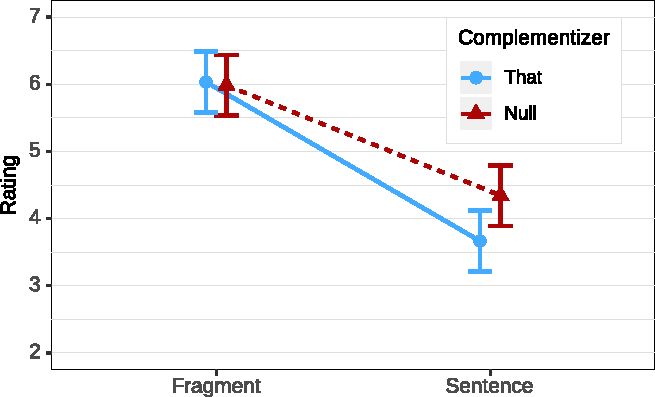
\includegraphics[scale=1]{figures/ex2b_ccs_en_estimates}
 \caption{Mean ratings and 95\% confidence intervals across conditions in experiment \ref{exp:ccs-english}. \label{fig:ccs-english-estimates}}
\end{figure}

The data were analyzed with CLMMs in \texttt{R} following the procedure described in Section \ref{sec:intro-stats}. I first fit a full model to the complete data set. The full model contained fixed effects for \textsc{Sententiality}, \textsc{CCType}, the \textsc{Position} of the trial in the time-course of the experiment and the \textsc{MatrixVerb} as well all two-way interactions between the IVs. The models had by-item random intercepts by-item random slopes for \textsc{Sententiality}, \textsc{CCType} and their interaction, as well as by-subject random intercepts and by-subject random slopes for \textsc{CCType}. By-subject random slopes for \textsc{Sententiality} were not considered, because \textsc{Sententiality} was tested as a between subjects IV. 

The final model (see Table \ref{tab:ccs-english-estimates}) contains significant main effects of \textsc{Sententiality}, \textsc{CCType}, \textsc{Position}, \textsc{MatrixVerb} and the \textsc{Sententiality:CC\is{Complement clause}Type} interaction. The main effect of \textsc{Sententiality} \clmmLR{29.85}{\highsig} confirms that fragments are preferred over topicalized CC\is{Complement clause}s. The main effect of \textsc{CCType} \clmmLR{10.58}{0.01} shows that, unlike it has been argued in the theoretical literature based on introspective data, complementizer omission\is{Complementizer omission} is overall preferred. Finally, the significant interaction between \textsc{Sententiality} and \textsc{CCType} \clmmLR{6.05}{0.05} shows that the preference for complementizer omission\is{Complementizer omission} is specifically strong for sentences. The \textsc{Position} effect \clmmLR{11.64}{0.001} reveals a slight overall improvement of ratings over time, but the absence of interactions with other predictors shows that this does not affect any condition in particular. The \textsc{MatrixVerb} main effect \clmmLR{7.6}{0.01} reveals a preference for materials with the matrix verb \textit{believe} as compared to other matrix verbs, for the other matrix verbs there was no such effect. Since the verb was not varied systematically across all items, this might be due to properties of individual materials, hence I consider this a control predictor. Just like in the German\is{German} experiments, I addressed the movement restriction\is{Movement restriction} with an analysis of the data for the full sentences only, following the same procedure as for the main analysis. The final model contains a \textsc{Position} effect \clmmLR{5.63}{0.05} and a main effect of \textsc{CCType} \clmmLR{13.7}{0.001} that confirms the preference for complementizer-less\is{Complementizer omission} clauses in a left-peripheral position.

\begin{table}[t]
\begin{tabular}{l l l l l l}
\lsptoprule
Predictor & Estimate & SE & $\chi^2$ &  $p$-value &  \\   
\midrule
\textsc{Sententiality} & \phantom{-}1.886 &  0.302 & 29.85 & \textless \highsig & *** \\
\textsc{CCType}  &  \phantom{-}0.443 &  0.13 & 10.58 & \textless 0.01 & ** \\
\textsc{MatrixVerb (believe)} &   \phantom{-}0.441 &  0.15  & \phantom{1}7.60 & \textless 0.01 & **\\ 
\textsc{Position}      &     \phantom{-}0.009 & 0.003   & 11.64 & \textless 0.001 & *** \\
\textsc{Sententiality:CC\is{Complement clause}Type} & -0.323 & 0.128  & \phantom{1}6.05 & \textless 0.05 & *\\
\lspbottomrule
\end{tabular}
\caption{Fixed effects in the final CLMM for experiment \ref{exp:ccs-english}. \label{tab:ccs-english-estimates}}
\end{table}

\newpage
\subsubsection{Discussion}
Like experiment \ref{exp:ccs-german}, experiment \ref{exp:ccs-english} investigated an assumed movement restriction\is{Movement restriction} on complementizer-less\is{Complementizer omission} CCs\is{Complement clause} that constrains the acceptability of the corresponding fragments according to \citet{merchant.etal2013}. The data do neither provide evidence for the assumed movement restriction\is{Movement restriction} nor for the effect that \citet{merchant.etal2013} report for fragments. The overall pattern in my English\is{English} data is similar to that found for German\is{German}: Short answers\is{Fragment, short answer} are preferred across the board and the overall difference in acceptability between \textsc{CCType} conditions is rather small in absolute terms. In English\is{English}, there was no difference in acceptability between both types of fragment CCs\is{Complement clause}. This contrasts with the study by \citet{merchant.etal2013}, who found such an effect, and suggests that the preference for CCs\is{Complement clause} with overt complementizers in their experiment was due to the use of factive\is{Factivity} matrix verbs, which disprefer complementizer-less\is{Complementizer omission} CCs\is{Complement clause}. Once more, there is no evidence for the movement restriction\is{Movement restriction} on which the study by \citet{merchant.etal2013} is based: Complementizer-less\is{Complementizer omission} CCs\is{Complement clause} were even rated\is{Acceptability rating task} as more acceptable that in the sentential conditions, whereas the opposite pattern has been repeatedly assumed in the theoretical literature based on introspective data.

\subsection{General discussion: Complementizer omission}
Experiments \ref{exp:ccs-german} and \ref{exp:ccs-english} investigated whether the presumed movement restriction\is{Movement restriction} on comple\-men\-tizer-less CCs\is{Complement clause} that \citet{merchant.etal2013} investigated indeed provides evidence for movement in fragments\is{Movement and deletion account}. The results suggest that it does not: First, there is no empirical evidence for the presumed movement restriction\is{Movement restriction} on complementizer-less\is{Complementizer omission} CCs\is{Complement clause}. Second, complementizer-less\is{Complementizer omission} CC\is{Complement clause} fragments are slightly degraded in German\is{German}, but this pattern is not reflected in the corresponding full sentences. In English\is{English}, there is no difference between fragments, and in full sentences the complementizer-less\is{Complementizer omission} CC\is{Complement clause} is even preferred. This suggests that \citet{merchant.etal2013} interpret their data based on incorrect assumptions and that the preference for realizing the complementizer in their materials is not related to movement restriction\is{Movement restriction}s.

The study by \citet{merchant.etal2013} differs from my experiments in three main aspects: First, the restriction to CCs\is{Complement clause} that are acceptable \textit{in situ}, that is complements of non-factive verbs\is{Factivity}, ensures that a possible preference for complementizer realization cannot be explained by \textit{in situ} deletion\is{In situ deletion account}. Degraded ratings for CCs\is{Complement clause} which are ungrammatical even \textit{in situ} are expected by \textit{any} ellipsis account. Second, the use of context stories ruled out the possibility of indirect answers, and third, I collected ratings for the left dislocation structures that \citet{merchant2004} assumes to be the source of fragments. \citet{merchant.etal2013} simply relied on the movement restriction\is{Movement restriction} on complementizer-less\is{Complementizer omission} CCs\is{Complement clause} reported in the literature. 

In both experiments, topicalized CCs\is{Complement clause} were rated\is{Acceptability rating task} as worse than fragments across the board, even though \textsc{CCType} was tested within subjects in order to attenuate this effect. None of the experiments confirmed the pattern reported in the literature with respect to topicalized CCs\is{Complement clause}: Both in English\is{English} and German\is{German} there were significant \textsc{Sententiality:CCType} interactions showing that the preference for realizing the complementizer is stronger in fragments than in left dislocation structures. The analyses of the sentential conditions in isolation show that complementizer-less\is{Complementizer omission} clauses were rated\is{Acceptability rating task} as more acceptable in the left-peripheral position in English\is{English}, and at least as acceptable in German\is{German} (in the follow-up to experiment \ref{exp:ccs-german} there was no significant difference). This is the opposite pattern to the one reported in the theoretical literature that underlies the interpretation of the data in \citet{merchant.etal2013}. If complementizer-less\is{Complementizer omission} CCs\is{Complement clause} are not dispreferred in a left-peripheral position, the preference for realizing the complementizer in fragments cannot be attributed to a movement restriction\is{Movement restriction}: No matter why we observe this pattern in fragments, it does not provide evidence for movement.

Rebecca Woods\ia{Woods, Rebecca} (p.c.) pointed out the possibility that the ratings for topicalized complementizer-less\is{Complementizer omission} CCs\is{Complement clause} improved because they were interpreted as parentheticals rather than as matrix clauses. Parentheticals do not subcategorize the embedding clause but can be inserted into regular verb-second clauses, hence it should be possible to omit the complementizer in that case. However, in the German\is{German} subjunctive conditions, which did not differ in acceptability\is{Acceptability rating task} from indicative, subjunctive mood marks the utterance as indirect speech. Since indirect speech is in general embedded under a matrix verb, a parenthetical reading of the matrix clause seems less appropriate in that case than with regular indicative verb-second clauses. If the indicative verb-second fragments were improved by the parenthetical interpretation, subjunctive should be to a lesser extent and hence rated\is{Acceptability rating task} worse. This is clearly not the case. In order to be completely sure however, the items would have to be modified in a way that rules out the parenthetical reading, for instance by including a negation in the matrix clause.

When only fragments are taken into account, the German\is{German}, but not the English\is{English}, data resemble those reported by \citet{merchant.etal2013}, even when controlling for factivity\is{Factivity}. In both German\is{German} experiments realizing the complementizer was preferred, whereas there was no significant effect of the complementizer on English\is{English} fragments. The difference in acceptability between conditions is smaller than in the experiment by \citet{merchant.etal2013} in absolute terms even though I used a 7-point scale instead of a 5-point scale. This might be due to the restriction to non-factive\is{Factivity} verbs, which are known to allow for complementizer omission\is{Complementizer omission}. Even though the results on sentence-initial CCs\is{Complement clause} do not evidence a movement restriction\is{Movement restriction}, a possible difference between German\is{German} and English\is{English} with respect to complementizer omission\is{Complementizer omission} might be investigated in future research.

Like the preposition omission\is{Preposition omission} data discussed in the previous section, my results do not \textit{falsify} the movement and deletion\is{Movement and deletion account} account. However, they challenge the interpretation of a relatively weak preference for realizing complementizers in short answer fragments\is{Fragment, short answer} when the experiment is replicated under more carefully controlled conditions as evidence for movement. The movement and deletion\is{Movement and deletion account} account can of course derive both fragment CCs\is{Complement clause} with and without complementizers from the corresponding left dislocations, which, unlike as has been argued in the literature, seem to be well-formed. However, there is no empirical evidence for the movement restriction\is{Movement restriction} assumed by \citet{merchant2004} and \citet{merchant.etal2013} that constrains the form of fragments. Therefore, even if the pattern predicted by \citet{merchant2004} is observed in some fragments (as it was by \citet{merchant.etal2013} and in experiment \ref{exp:ccs-german}), this cannot be traced back to a movement restriction\is{Movement restriction} on complementizer-less\is{Complementizer omission} complement clauses\is{Complement clause}. Since the movement and deletion\is{Movement and deletion account} account is derivationally more complex than \textit{in situ} deletion\is{In situ deletion account}, the absence of evidence for movement forces us to stick to the simpler \textit{in situ} deletion\is{In situ deletion account} account. If there is no movement restriction\is{Movement restriction} on complementizer-less\is{Complementizer omission} CCs\is{Complement clause}, this phenomenon may simply be the wrong testing ground for the movement and deletion\is{Movement and deletion account} account. For this reason, in Section \ref{sec:mvb} I explore whether a well-documented restriction on German\is{German} prefield\is{Prefield} configurations constrains the form of fragments.

\newpage
\section{Movement restrictions: The German prefield}\label{sec:mvb}
\subsection{The German prefield and movement in fragments}
The replications and extensions of the experiments by \citet{merchant.etal2013} question the assumption that preposition omission\is{Preposition omission} and complement clause\is{Complement clause} topicalization provide evidence for movement\is{Movement and deletion account}. In the case of preposition omission\is{Preposition omission}, the data can be explained without assuming movement by question-answer parallelism, and for complement clause\is{Complement clause} topicalization, there is no evidence for the presumed movement restriction\is{Movement restriction} itself. This section presents a last experiment on the syntax of fragments that investigates a well-documented movement restriction\is{Movement restriction} concerning the prefield\is{Prefield} position in German\is{German}. In a nutshell, the idea is that if the preverbal position in German\is{German} verb-second sentences is analyzed as the landing site for fragments, as \citet{merchant2004} suggests, only those constituents that can appear in this position are possible fragments.

\subsubsection{The prefield position in German verb-second clauses}
The German\is{German} declarative matrix clause is generally assumed to be strictly verb-second, so that only one constituent can precede the inflected verb. \is{Topological field model|(}Traditionally, this is modeled with the \textit{topological field model}\is{Topological field model} \citep{drach1937} of the German\is{German} sentence, which divides the sentence into three regions, the so-called \textit{fields}. These fields are delimited by two positions hosting verbal elements, the left and right \textit{brackets}. Table \ref{tab:feldermodell} shows how these fields are filled in declarative matrix clauses: The left bracket hosts the inflected verb and the right bracket the participle or infinitive, if the sentence contains such. The region left to the left bracket is called prefield\is{Prefield} and contains exactly one constituent, yielding the obligatory verb-second order. By default\is{Default case}, all other constituents appear in the middle field\is{Middle field}, the region between the brackets. In case of extraposition, constituents can be located in the postfield, i.e. in the region following the right bracket. \Next shows that, unlike in SVO languages, all arguments (including the subject) appear in the middle field\is{Middle field} if the prefield\is{Prefield} is filled by an adverbial\is{Adverbial}.\is{Topological field model|)}

\begin{table}[t]
\begin{tabular}{l l l l l l l l}
\lsptoprule
Prefield & LB & \multicolumn{2}{c}{Middle field} & RB & \multicolumn{3}{c}{Postfield}  \\   
\midrule
Peter & will & einen & Kuchen & backen & der & glutenfrei & ist\\
Peter & wants & a & cake & bake & that & gluten.free & is\\
\lspbottomrule
\end{tabular}
\caption{German topological fields model (LB = left bracket; RB = right bracket).\label{tab:feldermodell}}
\end{table}

\exg. Montag will Peter [einen Kuchen] backen, [der glutenfrei ist].\\
monday wants Peter a cake bake that gluten.free is\\
\trans{On Monday, Peter wants to bake a cake that is gluten-free.}

\newpage
\noindent In generative\is{Generative grammar} terms, the standard syntactic analysis of German\is{German} verb-second sentences assumes head movement of the verb from T to C followed by movement of the prefield\is{Prefield} constituent to [Spec, CP\is{Complementizer phrase}], as sketched in Figure \ref{ex:vorfeld-adv}.\largerpage[2]%
%
\footnote{This description is highly simplified. Furthermore, both the order of the movement operations and their motivation and casual connection (does one of them trigger the other, and if so, which?) have been controversially discussed (see \citet{brandner2004} for an overview of competing analyses of V2). In fact, Gereon \citet{muller2004} has argued that verb-second order is derived by remnant movement of the whole \textit{v}P to [Spec, CP\is{Complementizer phrase}] after the other constituents than the verb and the prefield\is{Prefield} constituents have been moved out for independent reasons. The resulting structure is given in \Next, taken from \citep[181]{muller2004}.

\ex. [\textsubscript{CP}\is{Complementizer phrase} [\textsubscript{vP}\textsubscript{5} Das Buch\textsubscript{2} \textit{t}\textsubscript{1} \textit{t}\textsubscript{4} hat\textsubscript{3} ] [\textsubscript{C'} C [\textsubscript{TP} Fritz\textsubscript{1} [\textsubscript{T'} [\textsubscript{VP}\textsubscript{4} \textit{t}\textsubscript{2} gelesen ] [\textsubscript{T'} \textit{t}\textsubscript{5} T]]]]]

\citeauthor{muller2004}'s account is not compatible with \citepos{merchant2004} version of movement and deletion\is{Movement and deletion account}. The E feature\is{E feature} on C would always cause the complete \textit{v}P to survive ellipsis, so that there would be no way of generating DP\is{Determiner phrase} fragments in German\is{German}. The corpus\is{Corpus} data by \citet{reich2017} and my previous experiments disconfirm this prediction. Note that this does not speak against \citeauthor{muller2004}'s analysis, unless movement and deletion\is{Movement and deletion account} is assumed.}\afterfn%
%

\begin{figure}[t]
 \Tree [.CP Montag\textsubscript{j} [.C' will\textsubscript{i} [.TP \edge[roof]; {Peter \textit{t}\textsubscript{j} einen Kuchen backen [\dots] \textit{t}\textsubscript{i}} ] ] ] 
 
 \caption{Following \citet{denbesten1989}, the verb-second word order of the German declarative matrix clause is the result of moving the inflected verb to C and another constituent to [Spec, CP].\label{ex:vorfeld-adv}}
\end{figure}

\subsubsection{The prefield position in the movement and deletion account}\label{sec:mvb-merchant}
\is{Complementizer omission|(}
In order to draw conclusions on the validity of the movement and deletion\is{Movement and deletion account} account from prefield\is{Prefield} configurations, it is crucial to assume that movement in fragments\is{Movement and deletion account} really targets the prefield\is{Prefield} according to \citeauthor{merchant2004}'s account. The structure in Figure \ref{ex:vorfeld-adv} differs from the one that \citet{merchant2004} assumes for English\is{English} because C and [Spec, CP]\is{Complementizer phrase} are always filled in regular German\is{German} declarative matrix sentences. In contrast, English\is{English} declarative matrix sentences are TPs\is{Tense phrase}, and the C head hosting E\is{E feature} is phonologically empty. Therefore, it is not immediately clear which position \citeauthor{merchant2004} identifies as the landing site for fragments in German\is{German}. In principle there are three options: First, like \citeauthor{merchant2004} suggested for English\is{English}, there could be an FP above CP\is{Complementizer phrase} and the E feature\is{E feature} could be located on C. Second, there could be an FP above CP\is{Complementizer phrase} and the E feature\is{E feature} be hosted by F. Finally, there could be no FP in German\is{German}, but an E feature\is{E feature} located on C that triggers movement of fragments to [Spec, CP]\is{Complementizer phrase}. All of these options are compatible with the theory, because \citet{merchant2004} suggests to account for crosslinguistic differences with respect to the availability and properties of ellipses by postulating differences in the specifications of the lexicon entries of the E feature\is{E feature}. 

For the German\is{German} verb-second clause, as the discussion in Section \ref{sec:theories-predictions-focus} showed, any analysis that locates the E feature\is{E feature} on C incorrectly predicts that the inflected verb survives ellipsis, because it is moved to C and only the complement of C is PF-deleted.%
%
\footnote{Note that this problem also concerns the exceptional movement\is{Exceptional movement account} version of the theory by \citet{weir2014}. \citeauthor{weir2014} can account better for the non-constituent fragments discussed in this section, because he simply adjoins\is{Adjunct} fragments to CP\is{Complementizer phrase} and there is no upper bound on the number of adjuncts. There might be constraints on the order of constituents in fragments, depending on whether the most deeply embedded focused constituents or the closest ones to the E feature\is{E feature} are fronted first. However, \citeauthor{weir2014} places the E feature\is{E feature} on C and consequently falsely predicts that finite verbs (which are also in C), as Figure \ref{ex:vorfeld-adv} shows, always survive ellipsis.}\afterfn%
%
In contrast, assuming an FP above CP\is{Complementizer phrase} and locating E\is{E feature} on F has the advantage of deleting the verb and thus being able to generate DP\is{Determiner phrase} fragments. However, it incorrectly predicts fragments to be insensitive to island\is{Island}s, because the defective trace\is{Trace (movement)} in [Spec, CP\is{Complementizer phrase}] would be deleted along the way. As for the third option, the assumption of an FP in German\is{German} lacks empirical support, because the prefield\is{Prefield} hosts only one constituent and fronted foci appear in the regular prefield\is{Prefield} \Next[a] instead of preceding other prefield\is{Prefield} constituents \Next[b]. If no FP is assumed in German\is{German}, this rules out the first two options listed above.

\ex. \ag. EINEN TOPF musst du nehmen, keine Pfanne!\\
	  a.\textsc{acc} pot must you take no pan\\
      \bg. *EINEN TOPF du musst nehmen, keine Pfanne!\\
	  a.\textsc{acc} pot you must take no pan\\
	  \trans{A POT you must take, not a pan!}
	 
\newpage
\noindent Furthermore, the identification of the landing site for fragments as [Spec, CP\is{Complementizer phrase}] is also implicitly adopted by \citet{merchant2004} himself. As I discussed in Section \ref{sec:theories-predictions-focus}, \citet[702]{merchant2004} presents parallelisms between the form of fragments in the prefield\is{Prefield} and in fragments as evidence for his account. This  implies that the presumed landing site for fragments is the regular prefield\is{Prefield}, that is, [Spec, CP\is{Complementizer phrase}].\is{Complementizer omission|)}

\refstepcounter{expcounter}\label{exp:mvb}
\subsection{Experiment \ref{exp:mvb}: Multiple prefield constituents}
\subsubsection{Background}\label{sec:mvb-background}
The German\is{German} prefield\is{Prefield} is a promising testing ground for movement and deletion\is{Movement and deletion account}: Since \citet{merchant2004} assumes it to be the landing site for fragments, only those expressions that can appear there in regular sentences can be grammatical fragments. Experiment \ref{exp:mvb} tested this hypothesis using the same method as in the experiments on CC\is{Complement clause} topicalization, i.e. by comparing the acceptability of fragments to that of the corresponding left dislocation structures.

Testing this prediction empirically requires establishing which expressions can and which ones cannot appear in the prefield\is{Prefield}. Since the prefield\is{Prefield} can be filled with most of the syntactic categories,%
%
\footnote{Only few expressions, such as modal particles, cannot appear there, as \Next shows.

\exg.*Wohl\textsubscript{i}/Ja\textsubscript{i} hat Peter \textit{t}\textsubscript{i} ein paar Leute eingeladen.\\
\textsc{prt} has Peter \mbox{} a few people invited\\
\trans{Peter has probably invited a few people.}\exsourceraised{\citep[227]{ott.struckmeier2016}}

}\afterfn%
%
the main restriction is that only a single constituent can precede the verb, because there is only one landing site in [Spec, CP\is{Complementizer phrase}]. In fact, the possibility of fronting an expression in verb-second clauses is often used as a constituency test in German\is{German}. 

Despite this, a corpus\is{Corpus}-based collection of multiple prefield\is{Prefield} constituents by Stefan Müller \citep{muller2002, muller2003, muller2005} shows that, at least superficially, the requirement of German\is{German} declarative matrix clauses to be verb-second is frequently violated. Three examples from \citet[32, 38, 59]{muller2003} are given in \Next. Some of these examples can probably be analyzed as single constituents, depending on the theoretical background that is assumed. However, in \Last[a], it seems odd to adjoin\is{Adjunct} a sentential adverb\is{Adverbial} to a DP\is{Determiner phrase}%
%
\footnote{But see \citet{bogal-allbritten2013} for an account of how modal adverbials\is{Adverbial} modify DPs\is{Determiner phrase}.}\afterfn%
%
and is it also not immediately clear that the locative and temporal adverbials\is{Adverbial} in \Last[b] are simply adjoined\is{Adjunct} to each other, as suggested by \citet{haider2000}. \Last[c] can be analyzed as VP\is{Verb phrase} fronting following movement of the verb to T or C, depending on where the adverbial \textit{des öfteren} is placed.%
%
\footnote{
\citeauthor{muller2003} excludes some apparent multiple prefield\is{Prefield} constituents from the set of problematic cases. For instance, \citet[21]{muller2003} argues that in \Next \textit{den Wagen} and \textit{zu reparieren} are not independent from each other, as accusative\is{Accusative case} on \textit{den Wagen} has to be licensed by the verb \textit{reparieren}. Therefore, what is fronted is a complete verbal projection and not two independent constituents. 

\exg. Den Wagen zu reparieren wurde versucht.\\
      the car to repair was tried\\
      \trans{It was intended to repair the car.} \exsourceraised{\citep[21]{muller2003}}

}\afterfn%
%
In fact, \citet[13--22]{muller2005} himself argues that such prefield\is{Prefield} configurations constitute a single constituent headed by a phonologically null verb. 

\ex. \ag. [Vermutlich] [vom    gleichen  Täter]    wurden zwei Tankstellen in Hemsbach und Heidelberg überfallen.\\
probably of.the  same criminal were two gas.stations in Hemsbach and Heidelberg assaulted\\
\trans{Probably by the same criminal two gas stations in Hemsbach and Heidelberg were assaulted.}
\bg. [Vor drei  Wochen] [in Memphis] hatte Stich noch in drei Sätzen gegen Connors verloren.\\ 
before three weeks    in Memphis  had   Stich  still   in three sets   against Connors lost\\
\trans{Three weeks ago in Memphis Stich had still lost in three sets against Connors.}
\cg. [Studenten] [einem Lesetest] unterzieht er des öfteren.\label{ex:muller-vf-doio} \\ 
students a reading.test  submits he the more.frequent\\
\trans{Students a reading test he submits frequently.}

From the perspective of an empirical investigation of movement and deletion\is{Movement and deletion account} however, it is irrelevant how apparent multiple prefield\is{Prefield} constituents are analyzed: If the German\is{German} prefield\is{Prefield} is the landing site for fragments, the movement and deletion\is{Movement and deletion account} account predicts that only those expressions that can somehow be moved there are possible fragments. Experiment \ref{exp:mvb} tests this prediction by comparing three instances of multiple prefield\is{Prefield} configurations that \citet{muller2003} classifies as acceptable to two of those he argues that are ungrammatical. Again, these prefield\is{Prefield} configurations are tested both as fragments and in sentences.\largerpage

\subsubsection{Materials}\label{sec:mvb-method}

Experiment \ref{exp:mvb} investigates five different prefield\is{Prefield} configurations in an acceptability rating\is{Acceptability rating task} study. Since multiple prefield\is{Prefield} configurations are restricted to specific information-structural\is{Information structure} contexts \citep{muller2005, bildhauer2011}, all critical utterances were preceded by a context that elicited the appropriate information structure\is{Information structure}. For instance, in  \Next, where both the direct and indirect object are fronted, \citet[59]{muller2003} notes that the first prefield\is{Prefield} constituent \textit{seinem Chef} `his boss' must be a contrastive topic\is{Topic, contrastive} \citep{buring1997} and the second one \textit{eine E-Mail} `an e-mail' a contrastive focus\is{Focus, contrastive}. 
The context question in \Next[a] intended to rule out the possibility that the utterance is inappropriate in out-of-the-blue contexts by information-structural\is{Information structure}ly licensing the marked word order\is{Word order}. Each item was tested as a fragment \Next[b] and in the prefield\is{Prefield} of a full sentence \Next[c].

\ex. Direct and indirect object \label{ex:mvb-item-doio}
\ag. Hätte  er  der Personalabteilung ein Fax schicken sollen?\\
has.\textsc{sbjv} he the HR.department a fax send shall\\
\trans{Should he have sent a fax to the HR department?}
\bg. Nein, seinem Chef eine E-Mail.\\
    no  his  boss an  e-mail\\
    \trans{No, his boss an e-mail.}
\cg. Nein, seinem Chef eine E-Mail hätte er schicken sollen.\\
	no his boss an  e-mail   has.\textsc{sbjv} he send shall\\
\trans{No, his boss an e-mail he should have sent.}

The experiment tested three prefield\is{Prefield} configurations that are grammatical according to \citet{muller2005} (direct + indirect object \Last, local + temporal adverbial\is{Adverbial} \ref{ex:mvb-item-loctemp} and argument + sentential adverb \ref{ex:mvb-item-sadvxp}) and two that are not (subject + other argument DP\is{Determiner phrase} \ref{ex:mvb-item-subjxp} and non-clausemates \ref{ex:mvb-item-diffcl}). Some of these conditions might be analyzed as involving a single constituent in the prefield\is{Prefield}: The cooccurrence of a locative and a temporal adverbial\is{Adverbial} \ref{ex:mvb-item-loctemp} could be analyzed as adjoined\is{Adjunct} to each other, but semantically both modify the remaining clause and not one of them the other one. In the sentential adverb and argument condition \NNext, the adverb\is{Adverbial} \textit{angeblich} `allegedly' takes scope over \textit{in seiner Stammkneipe} `in his favorite pub' only. This might indicate that it forms a constituent with the noun or DP\is{Determiner phrase}. \citet[31]{muller2003} nevertheless cites \ref{ex:muller-jacobs} by \citet[112]{jacobs1986} for evidence that sentential adverbs cannot occur inside a PP\is{Preposition phrase}. This indicates that they may be semantically associated with the noun, but not syntactically. After all, the purpose of the experiment is not to isolate prefield\is{Prefield} configurations that are equally acceptable but to investigate whether acceptability differences among them are reflected in the acceptability of fragments.

\newpage
\ex. Locative and temporal adverbial\is{Adverbial}\label{ex:mvb-item-loctemp}
\ag. Wann hast  du   Hans denn getroffen? \\
when have you Hans  then  met\\
\trans{So when did you meet Hans?}
\bg. [Heute morgen  in der U-Bahn] habe ich ihn getroffen.\\
today   morning in the subway  have I    him met\\
\trans{This morning in the subway I met him.}

\ex. Sentential adverb\is{Adverbial} and argument XP\label{ex:mvb-item-sadvxp}
\ag. Wo  war Herr Veit zum   Tatzeitpunkt?\\
    where  was Mr    Veit to.the time.of.crime\\
\trans{Where was Mr Veit at the time of the crime?}
\bg. [Angeblich in seiner  Stammkneipe] war er  zum  Tatzeitpunkt.\\
allegedly in his favorite.pub was he to.the time.of.crime\\
\trans{Allegedly in his favorite pub he was at the time of the crime.}

\exg. *Peter träumt von (vermutlich/ sogar/ nicht) (ihr/ Luise/ Geld).\\  
 Peter dreams of probably/ even/ not her/ Luise/ money\\
\trans{Peter dreams of probably/even/not her/Luise/money.}\label{ex:muller-jacobs}

The two ungrammatical prefield\is{Prefield} configurations are given in \Next and \NNext. As for \Next, \citet[59]{muller2003} notes that a preverbal subject and an additional argument cannot appear together in the prefield\is{Prefield}. The ungrammatical configuration in \NNext involves the extraction of two constituents from different clauses to the prefield\is{Prefield}. This violates the requirement of prefield\is{Prefield} constituents to be clause-mates \citep{fanselow1993}. In \NNext, \textit{den Hund} `the dog' is the direct object of the embedded verb \textit{ärgern} `to bother', while \textit{Paul} is the indirect object of the matrix verb \textit{verbieten} `to forbid'. Note that, unlike in \Next, there is no subject involved in the multiple prefield\is{Prefield} sequence in \NNext. The prefield\is{Prefield} configuration itself should thus be acceptable if the constituents were not extracted from different clauses, as in \ref{ex:mvb-diffcl-nondiff}, because it consists of the direct and the indirect object like the presumably grammatical \ref{ex:mvb-item-doio}.

\ex. Subject and argument XP \label{ex:mvb-item-subjxp}
\ag. Wer möchte welche Aufgabe übernehmen? \\
    who wants   which   task        take.on\\
	\trans{Who wants to take on which task?}
	\bg. *[Ich die Spülmaschine] möchte übernehmen.\\
   I  the dishwasher   want     take.on \\
	\trans{I want to take on the dishwasher.}
	
\ex. Extraction out of different clauses \label{ex:mvb-item-diffcl}
\ag. Wem   hast  du   verboten, wen zu ärgern?\\
    whom  have you forbidden who to  bother\\
	\trans{Who did you forbid to bother who?}
	\bg. *[Paul den Hund] habe  ich verboten, zu ärgern.\\
     Paul   the  dog     have  I     forbidden to bother\\
	\trans{I forbade Paul to bother the dog.}
	
\exg. Paul den Hund habe ich geschenkt. \label{ex:mvb-diffcl-nondiff}\\
    Paul the  dog    have I    given.as.present\\
   \trans{I gave Paul the dog (as present).}

It shall be noted that \citet[710--711]{merchant2004} briefly discusses the (introspective) observation that short answer fragments\is{Fragment, short answer} to multiple \textit{wh}-questions are relatively acceptable even though the corresponding multiply filled prefield\is{Prefield} is heavily degraded. Without going into details, he suggests that this also evidences repair effects by ellipsis. I address this in the discussion of this experiment.

\subsubsection{Procedure}
The experiment was completed by 38 undergraduate students of Saarland University. All were native speakers of German\is{German}. They were rewarded with the participation in a lottery of 5 $\times$ \currencyEuro{30.00} among all participants. The experiment was conducted in the same session as the production study\is{Production task} on case marking (experiment \ref{exp:case-production}), where subjects were asked to produce utterances referring to graphical stimuli. Subjects were asked to rate the naturalness of the italicized target utterance in the context of the question on a 7-point Likert scale (7= fully natural). In order to prevent possible floor effects, \textsc{Sententiality} was tested as a between subjects variable. Each subject rated\is{Acceptability rating task} 35 items (7 per \textsc{Prefield}\is{Prefield} configuration). The materials were presented together with 21 items of the follow-up to experiment \ref{exp:ccs-german} and 25 unrelated fillers including four ungrammatical controls in individually pseudo-randomized order. A pseudo-randomized presentation ensured that no two items of the same experiment followed each other. Fillers were adapted so as to match the \textsc{Sententiality} of the materials in the list, so that subjects saw either only sentential or only fragment target utterances. This also matched the design of the follow-up to experiment \ref{exp:ccs-german}, which had the same manipulation. One participant rated\is{Acceptability rating task} 50\% or more of the ungrammatical controls with 6 or 7 points on the scale and was therefore excluded from further analysis. 

\begin{figure}[t]
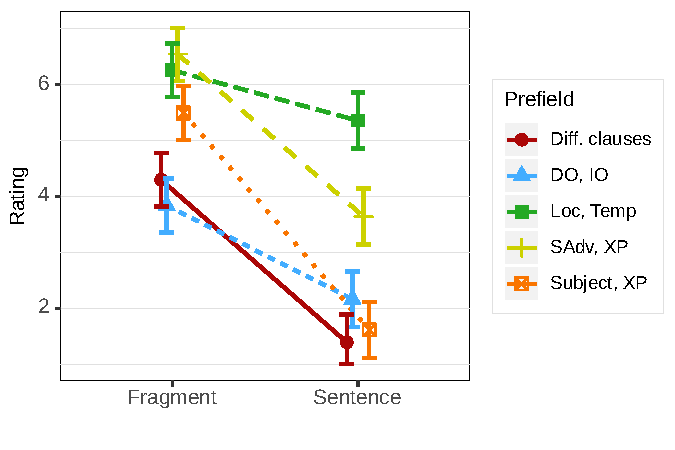
\includegraphics[scale=1]{figures/ex3_mvb_estimates}
 \caption{Mean ratings and 95\% confidence intervals across conditions in experiment \ref{exp:mvb}.\label{fig:mvb-estimates}}
\end{figure}

\subsubsection{Results}\label{sec:mvb-results}
Figure \ref{fig:mvb-estimates} shows that across all conditions fragments were rated\is{Acceptability rating task} better than sentences and that there was a large extent of variation between conditions. Specifically, the presumably ungrammatical conditions and grammatical conditions do not behave uniformly: The grammatical \textsc{SAdv, XP} and the grammatical \textsc{LocAdv, TempAdv} are both almost equally acceptable as fragments, but strongly differ as prefield\is{Prefield} configurations. Due to these differences, it would not be appropriate to pool the presumably ungrammatical and grammatical conditions. Instead, I conducted pairwise comparisons between each two of the conditions, yielding a series of 10 2$\times$2 contrasts (\textsc{Sententiality}$\times$\textsc{Prefield}) that I analyzed separately. For each of these contrasts I statistically analyzed a subset of the data containing only those data points belonging to the respective condition with CLMMs according to the procedure described in Section \ref{sec:intro-stats}.

\begin{table}[t]
  \begin{tabular}{p{2cm} p{2cm}p{2cm}p{2cm}p{2cm}p{2cm}}
   \lsptoprule
   & \textsc{Subj, XP} & \textsc{SAdv, XP} & \textsc{Loc, Temp} & \textsc{DO, IO}\\
      \midrule
  \textsc{Non-CM}  & n.s. & n.s. & \clmmLRbr{11.52}{0.001} & \clmmLRbr{15.77}{\highsig} \\
  \textsc{DO, IO}  & \clmmLRbr{15.73}{\highsig} & \clmmLRbr{10.95}{0.001} & n.s. & \greycell \\
  \textsc{Loc, Temp} & \clmmLRbr{14.66}{0.001} & \clmmLRbr{11.32}{0.001} & \greycell  & \greycell \\
  \textsc{SAdv, XP} &  n.s.\linebreak~~ & \greycell & \greycell& \greycell \\
  \lspbottomrule
 \end{tabular}
\caption{Significance of the pairwise comparisons between prefield configurations. P-values were Bonferroni-corrected, i.e. multiplied by the number of comparisons ($n = 10$).\label{tab:mvb-interactions}}
\end{table}

\newpage
\noindent The initial model for each data set contained main effects for \textsc{Sententiality} and \textsc{Prefield}\is{Prefield} as well as the interaction between these predictors. As for by-subject random effects I included only the intercept and a slope for \textsc{Prefield}\is{Prefield}, since \textsc{Sententiality} had been tested between subjects. Similarly, I included by-item random intercepts and slopes for \textsc{Sententiality}, because \textsc{Prefield}\is{Prefield} was not varied between items. The crucial predictor is the \textsc{Sententiality:Prefield}\is{Prefield} interaction, which indicates that the difference between conditions cannot be explained solely by a theoretically uninteresting overall preference for fragments or the markedness of a specific construction. Since the movement and deletion\is{Movement and deletion account} account predicts that only those prefield configurations which are acceptable as such yield grammatical fragments, it predicts no such interactions.

Table \ref{tab:mvb-interactions} summarizes the pairwise comparisons. Due to multiple comparisons, the reported p-values were Bonferroni-corrected, that is, multiplied by the number of comparisons ($n~=~10$). First of all, in most of the pairwise comparisons there are significant \textsc{Sententiality:Prefield}\is{Prefield} interactions. The pattern in Table \ref{tab:mvb-interactions} suggests that there is a split between conditions, but that this split does not occur between those prefield configurations that are grammatical and those that are ungrammatical according to \citet{muller2003}. The \textsc{Sententiality:Prefield}\is{Prefield} interactions are significant for any comparison between \textsc{Loc, Temp} and \textsc{DO, IO} and the remaining three predictors, but not between these two predictors. There are no significant interactions in the comparisons between the other three predictors. This suggests that the preference for the fragment is stronger in the two presumably ungrammatical prefield conditions and in \textsc{SAdv, XP}.

\subsubsection{Discussion}\label{sec:mvb-discussion}
Experiment \ref{exp:mvb} tested whether movement restrictions\is{Movement restriction} on German\is{German} multiple prefield\is{Prefield} configurations, which have not been investigated from this perspective previously, constrain the form of fragments. The idea underlying the experiment is that, if the movement and deletion\is{Movement and deletion account} account is correct, only those expressions that may appear in the preverbal position in German\is{German} verb-second clauses yield acceptable fragments. Statistically, this would be reflected in the absence of \textsc{Sententiality:Prefield} interactions between conditions.

As Table \ref{tab:mvb-interactions} shows, however, there are significant interactions in six out of ten pairwise comparisons. These interactions are unexpected under a movement and deletion\is{Movement and deletion account} account, but they do not ultimately falsify it, because some of the data points are close to the extremes of the scale and thus could reflect ceiling and floor effects, respectively. However, there are three conditions which are close to the mean rating for ungrammatical controls ($\mu = 1.79$) for sentences and ($\mu = 2.25$) for fragments,%
\footnote{\textsc{Sententiality} was tested between subjects, so that I present separate mean ratings for ungrammatical controls in each of the two groups.}\afterfn%
%
and among these specifically the \textsc{Subj, XP} condition yields acceptable fragments.

These interactions arise specifically when comparing the presumably grammatical prefield\is{Prefield} conditions (which involve the fronting of at least one adverbial\is{Adverbial}) to the ungrammatical ones (which involve the fronting of more than one DP\is{Determiner phrase}) and show that fragments that \citet{merchant2004} would derive from ungrammatical prefield\is{Prefield} configurations are rated\is{Acceptability rating task} as better than expected based on the main effects only. This contradicts the prediction of the movement and deletion\is{Movement and deletion account} account and is specifically pronounced for the \textsc{Subj, XP} condition, which is as degraded as ungrammatical fillers in the sentence condition, but more acceptable than the grammatical \textsc{DO, IO} if it appears as a fragment. The \textsc{SAdv, XP} condition seems to be somehow special, as it patterns with the ungrammatical conditions with respect to the relative preference for fragments, but is based on a possibly grammatical prefield\is{Prefield} configuration. Taken together, the experiment shows that some prefield\is{Prefield} configurations which are clearly ungrammatical are the presumed underlying structure of well-formed fragments.

Although this seems to challenge the movement and deletion\is{Movement and deletion account} account, \citet[710--711]{merchant2004} argues that fragments derived from multiple prefield\is{Prefield} constituents evidence repair effects. The mechanism he proposes for the repair of island\is{Island} violations could potentially explain the data from the non-clausemates condition. If the embedded clause in \ref{ex:mvb-item-diffcl}, repeated here for convenience as \Next, is an island\is{Island}, extraction of the DP\is{Determiner phrase} \textit{den Hund} out of it will leave a defective trace\is{Trace (movement)}, in the [Spec, CP\is{Complementizer phrase}] of the embedded clause. This trace\is{Trace (movement)} is deleted by ellipsis on PF, so that the derivation is saved. Still though, it is unclear how \textit{Paul} and \textit{den Hund} would be merged to a single constituent that can appear in the prefield\is{Prefield}.

\exg.  *[Paul den Hund] habe  ich verboten, zu ärgern. \\
     Paul   the  dog     have  I     forbidden to bother\\
	\trans{I forbid Paul to bother the dog.}

The case of the \textsc{Subj, XP} condition is even harder to explain from a movement and deletion\is{Movement and deletion account} perspective, because deriving fragments from a verb-second sentence is intricate, as the discussion in Section \ref{sec:mvb-merchant} showed. Under a standard analysis of German\is{German} verb-second word order\is{Word order}, fragments cannot target the prefield\is{Prefield} in [Spec, CP\is{Complementizer phrase}] because this would falsely predict that the finite verb also survives ellipsis after raising to C. Furthermore, if the subject is fronted in a matrix clause, as it is in the \textsc{Subj, XP} conditions, there is no such defective trace\is{Trace (movement)} that would be deleted by ellipsis. The only solution in terms of movement and deletion\is{Movement and deletion account} is the stipulation of a functional projection above CP\is{Complementizer phrase}, whose head hosts the E feature\is{E feature} and whose specifier is the landing site for fragments. However, such a projection (i) would be specific to ellipsis, (ii) would predict fragments to be island\is{Island}-insensitive, and (iii) is not in line with \citet{merchant2004}, who identifies the regular prefield\is{Prefield} as the landing site for fragments. The more stipulations lacking independent evidence have to be made in order to reconcile the data with the predictions of the movement and deletion account\is{Movement and deletion account}, the less explanatory adequate is the theory.

If the movement and deletion\is{Movement and deletion account} account fails to account for the data, the obvious question is whether the other theories discussed so far do better. \citepos{reich2007} \textit{in situ} deletion\is{In situ deletion account} account can explain the observed pattern because the close relationship between question and answer in terms of focus structure is central to his theory. The constituents that survive ellipsis correspond to \textit{wh}-phrases in the context question and are therefore focused, or at least not given, as in case of the adverbials\is{Adverbial} which are not included in the question. In contrast, the part of the sentence that is omitted in the fragment is backgrounded by the question. \textit{In situ} deletion\is{In situ deletion account} hence predicts all fragments tested in experiment \ref{exp:mvb} to be grammatical. The observation that some of the prefield\is{Prefield} configurations are more acceptable than others does not concern \textit{in situ} deletion\is{In situ deletion account}, because it derives fragments from regular sentences with only one prefield\is{Prefield} constituent. \citepos{weir2014} exceptional movement\is{Exceptional movement account} account in principle makes a similar prediction, because he argues that all focused constituents are adjoined\is{Adjunct} to CP\is{Complementizer phrase} when they are moved out of the ellipsis site.

\noindent The nonsentential account\is{Nonsentential account} might be able to account for those of the fragments that can somehow be analyzed as forming a constituent. This concerns the conditions involving adverbials\is{Adverbial}, if adverbials\is{Adverbial} are analyzed as adjoined\is{Adjunct} to each other in the \textsc{Loc, Temp} condition and to the DP\is{Determiner phrase} in the \textsc{SAdv, XP} condition. It is unclear how \citet{barton.progovac2005} would account for the DP\is{Determiner phrase}-DP\is{Determiner phrase} fragments in three out of the five conditions. This is particularly relevant for the \textsc{NonClausemates} and \textsc{Subj, XP} conditions, for which a small clause\is{Small clause} analysis seems to be impossible, because the base positions of the involved constituents are definitely distant from each other. Taken together, the multiple prefield\is{Prefield} data contradict the movement and deletion account\is{Movement and deletion account} and the nonsentential account\is{Nonsentential account}, but they are in line with \textit{in situ} deletion\is{In situ deletion account}.

\section{The syntax of fragments: Discussion}\label{sec:syntax-gdiscussion}
This chapter presented a total of 10 experiments that empirically investigated predictions of the competing theories of fragments discussed in Chapter \ref{sec:chapter-theories}. The experiments addressed two main research questions that differentiate between the theories: First, whether fragments are sentential, and second, whether their derivation requires obligatory movement. The first question was investigated by using structural case\is{Structural case} marking on DP\is{Determiner phrase} fragments as evidence for an unarticulated verbal head. Experiments \ref{exp:case}--\ref{exp:scripts-rating-case} provide evidence for such unarticulated structure. The second question was investigated at the case of three movement restrictions\is{Movement restriction} which the movement and deletion\is{Movement and deletion account} account predicts to affect the acceptability of fragments: A ban on preposition omission\is{Preposition omission} in German\is{German} (experiments \ref{exp:pstranding-german}--\ref{exp:pstranding-production}), a crosslinguistic restriction on topicalizing complementizer-less\is{Complementizer omission} CCs\is{Complement clause} (experiments \ref{exp:ccs-german} and \ref{exp:ccs-english}), and restrictions on multiple prefield\is{Prefield} constituents in German\is{German} (experiment \ref{exp:mvb}). Taken together, these experiments find no clear evidence for movement and deletion\is{Movement and deletion account} and in conjunction with the experiments on sententiality support the \textit{in situ} deletion\is{In situ deletion account} account. In what follows I  discuss the main results and their relevance to my experiments on the usage of fragments in Chapter \ref{sec:chapter-infotheory-experiments}.

\subsection{Fragments are sentential}
The experiments in Section \ref{sec:experiments-case} investigated case connectivity\is{Case connectivity} as potential evidence for unarticulated structure in fragments at the example of accusative\is{Accusative case} structural case\is{Structural case} in German\is{German}. Accusative is assigned to the complement of transitive verbs, hence accusative\is{Accusative case} case marking on DP\is{Determiner phrase} fragments evidences the existence of an unarticulated verbal head in fragments. 
Experiment \ref{exp:case} showed that fragments in German\is{German} can appear in accusative\is{Accusative case} structural case\is{Structural case} even in the absence of linguistic context\is{Context, linguistic}. Experiment \ref{exp:case-production} confirmed the availability of a salient antecedent in the materials. Since the experiments show that accusative\is{Accusative case} structural case\is{Structural case} is acceptable, they support a sentential account of fragments. This interpretation relies on the assumption that the German\is{German} accusative\is{Accusative case} is structural case\is{Structural case}. \citet{progovac.etal2006} question this for Serbian\is{Bosnian/Croatian/Serbian}, but I showed that their diagnostics yield the opposite result for German\is{German}. 

Some of the experiments designed to test the movement and deletion\is{Movement and deletion account} account also speak against the nonsentential account\is{Nonsentential account}. Experiment \ref{exp:pstranding-defaultcase} tested a potential explanation for the impossibility of omitting prepositions\is{Preposition omission} in German\is{German} short answers\is{Fragment, short answer} if the \textit{wh}-phrase in the question is embedded within a PP\is{Preposition phrase}. If prepositional case\is{Prepositional case} is structural case\is{Structural case}, which must be checked by the preposition, \citet{barton.progovac2005} predict that DP\is{Determiner phrase} fragments in prepositional case\is{Prepositional case} are ungrammatical. In contrast, nominative\is{Nominative case} default case-marked DP\is{Determiner phrase}s are expected to be grammatical. The experiment clearly disconfirms this prediction, because nominative\is{Nominative case} is rated\is{Acceptability rating task} as even worse than prepositional case\is{Prepositional case} in the absence of a preposition. \citet{progovac.etal2006} argue that default case might be sometimes degraded for pragmatic reasons, but the theory would still predict a pragmatically odd expression to be more acceptable than an ungrammatical one.

Experiment \ref{exp:mvb} showed that some apparently discontinuous fragments, DP\is{Determiner phrase}-DP\is{Determiner phrase} sequences like \textit{Ich die Spülmaschine} `Me the dishwasher' are acceptable in appropriate contexts. Since fragments have to be maximal projections according to the nonsentential theory\is{Nonsentential account}, it is unclear how it would account for non-constituent fragments. The small clause\is{Small clause} analysis that \citet{progovac2006} proposes fails to explain the data, because (i) the second DP\is{Determiner phrase} is not the  complete predicate of the first one, and (ii) \citet{reich2017} discards a small clause\is{Small clause} analysis in German\is{German} for theoretical and empirical reasons. Another possible account is \citepos{muller2003} suggestion of an empty verbal head, but the idea of the nonsentential account\is{Nonsentential account} is obviously to do without unarticulated structure.

Finally, experiment \ref{exp:scripts-rating-case} addressed the possibility of a mixed account\is{Mixed account} of fragments that restricts the nonsentential derivation of fragments to contexts where no antecedent for ellipsis (resolution) is available. Such an account would predict that accusative\is{Accusative case} on DP\is{Determiner phrase} fragments is licensed only in contexts where a salient antecedent is available and that fragments appear in nominative\is{Nominative case} default case\is{Default case} otherwise. The experiment disconfirms this prediction, as accusative\is{Accusative case} is preferred to the same extent in both types of contexts. 

\newpage
\noindent Taken together, the experiments on the syntax of fragments presented so far disconfirm the central predictions that distinguish the nonsentential account\is{Nonsentential account} from its competitors: Neither is structural case\is{Structural case} unavailable in fragments, nor is default case\is{Default case} preferred over ungrammatical alternatives. I take this as evidence that fragments are elliptical sentences.

\subsection{Fragments are not obligatorily moved}
In Sections \ref{sec:pstranding}--\ref{sec:mvb} I presented a series of experiments that investigated how the unarticulated structure in fragments looks like. These experiments tested potential evidence for the influential movement and deletion\is{Movement and deletion account} account by \citet{merchant2004}, which assumes that the derivation of fragments involves obligatory movement to the left periphery before ellipsis applies. I pursued the approach that the alternative, \textit{in situ} deletion\is{In situ deletion account}, is the null hypothesis because this theory is derivationally simpler. Movement will only be assumed if there is empirical evidence that the \textit{in situ} deletion\is{In situ deletion account} account cannot explain. All experiments on movement follow the line of reasoning that movement would be evidenced by effects of movement restrictions\is{Movement restriction} on the form of fragments, as \citet{merchant2004} suggests. I investigated three instances of movement restrictions\is{Movement restriction}: obligatory pied-piping\is{Pied-piping} of prepositions (experiments \ref{exp:pstranding-german}--\ref{exp:pstranding-production}), complement clause\is{Complement clause} topicalization (experiments \ref{exp:ccs-german} and \ref{exp:ccs-english}) and restrictions and different configurations in the German\is{German} prefield\is{Prefield} (experiment \ref{exp:mvb}).

The first series of experiments addressed the P-Stranding Generalization\is{P-Stranding Generalization} \citep{merchant2001,merchant2004}, which states that only those languages that have P-stranding\is{Preposition stranding} allow for the omission of prepositions\is{Preposition omission} in short answers\is{Fragment, short answer}. Experiments \ref{exp:pstranding-german} and \ref{exp:pstranding-english} confirm the introspective pattern reported in the literature: In German\is{German}, the preposition cannot be omitted\is{Preposition omission} in short answers\is{Fragment, short answer} to questions where the \textit{wh}-phrase is the complement of a preposition. In contrast, in English\is{English} the preposition can be stranded\is{Preposition stranding} in the question, and when it is, omission is possible and actually preferred. Experiment \ref{exp:pstranding-production} tested whether this pattern can be explained without the assumption of movement in short answers\is{Fragment, short answer} by a structural parallelism between questions and answers. Structural parallelism provides a non-movement explanation for the PSG\is{P-Stranding Generalization}: In German\is{German}, DP\is{Determiner phrase} short answers\is{Fragment, short answer} to PP\is{Preposition phrase} questions are unavailable because the preposition always appears as the complement of P in the question. This approach makes the testable prediction that the form of the answer matches that of the question in languages where P-stranding\is{Preposition stranding} is available. There are two possible accounts of question-answer parallelism: a semantic one based on the idea that questions denote structured propositions \citep{reich2002}, and a psycholinguistic one, which builds on the observation that interlocutors reuse structure from previous discourse \citep{levelt.kelter1982}. Under both of these approaches, there is a nonsyntactic relationship between the availability of P-stranding\is{Preposition stranding} in the question and the preference for preposition omission\is{Preposition omission} in the answer. Experiment \ref{exp:pstranding-production} revealed an effect of the form of the question on that of the answer, just like question-answer parallelism predicts, which is line with the corpus\is{Corpus} data in \citet{nykiel2017}. The evidence for question-answer parallelism does not \textit{falsify} the movement and deletion\is{Movement and deletion account} account but it provides an explanation for the data under the derivationally simpler \textit{in situ} deletion\is{In situ deletion account} account.

As for complement clause\is{Complement clause} topicalization, \citet{merchant.etal2013} showed that an apparently well-established movement restriction\is{Movement restriction} on the topicalization of complement clause\is{Complement clause}s that lack an overt complementizer is in line with the acceptability of the corresponding fragments. Experiments \ref{exp:ccs-german} and \ref{exp:ccs-english} replicate their experiment in English\is{English} and German\is{German} under more controlled conditions. First, only complement clause\is{Complement clause}s which are grammatical \textit{in situ} are tested, second, ratings for the corresponding left dislocation structures are collected as well, and third, context stories ruled out the possibility of indirect answers. Experiment \ref{exp:ccs-german} confirms the effect reported by \citet{merchant.etal2013} for German\is{German} fragments, but the data for left dislocations provide no evidence for the alleged movement restriction\is{Movement restriction}. In English\is{English} (experiment \ref{exp:ccs-english}), both types of fragments were equally acceptable and the pattern for left dislocations resulted to be the opposite of that reported in the literature. Hence, any effects found in fragments must be attributed to other parameters than a movement restriction\is{Movement restriction}.

Finally, experiment \ref{exp:mvb} tested whether restrictions on multiple prefield\is{Prefield} constituents in German\is{German} constrain the acceptability of the corresponding fragments. Again, this is not the case. Specifically, the ungrammatical prefield\is{Prefield} configuration of a subject and a further argument DP\is{Determiner phrase} is acceptable as a fragment and there is no obvious explanation for this under the movement and deletion\is{Movement and deletion account} account.

None of the three potential sources of evidence for movement that I investigated provides evidence for movement in fragments\is{Movement and deletion account}: The P-stranding\is{Preposition stranding} data are in line with the movement and deletion\is{Movement and deletion account} account, but can also be explained by question-answer parallelism. The alleged movement restriction\is{Movement restriction} on topicalization could not be empirically demonstrated, and multiple prefield\is{Prefield} configurations that are ungrammatical result in acceptable fragments. Furthermore, from a more theoretical perspective, the derivation of fragments from German\is{German} verb-second sentences turned out to entail unsolved theoretical issues that concern the location of the E feature\is{E feature} in the German\is{German} left periphery and empirically false predictions resulting from that.

\subsection{Conclusion and outlook}

Taken together, experiments \ref{exp:case}--\ref{exp:mvb} favor the \textit{in situ} deletion\is{In situ deletion account} account by \citet{reich2007}. Specifically,the experiments that investigate movement restrictions\is{Movement restriction} find no evidence for the parallelism between the acceptability of left dislocation and the corresponding fragments that underlies the arguments in \citet{merchant2004}. This may be accounted for by the exceptional movement\is{Exceptional movement account} version of the movement \citep{weir2014}, but since the derivationally simpler \textit{in situ} deletion\is{In situ deletion account} account can explain the data as well, the assumption of an additional movement step is unmotivated and does not improve the empirical coverage of the theory. As for the nonsentential account\is{Nonsentential account}, I focused on the version proposed by \citet{barton.progovac2005}. The predictions of this theory are disconfirmed by experiments \ref{exp:case}--\ref{exp:scripts-rating-case}, which show that DP\is{Determiner phrase} fragments can appear in structural case\is{Structural case}, and experiment \ref{exp:pstranding-defaultcase}, which rules out the nonsentential account\is{Nonsentential account}'s case checking\is{Case feature}-based account of the PSG\is{P-Stranding Generalization}. Nonsentential accounts operating in different frameworks \citep[e.g.][]{ginzburg.sag2000, fernandez.ginzburg2002, culicover.jackendoff2005} might still be able to explain the data.

From a more agnostic theoretical perspective, the experiments presented so far evidence some properties of fragments which have been controversially discussed in the literature. First, since fragments are derived by ellipsis, they receive the same morphological marking as in the corresponding sentences. Second, an \textit{in situ} deletion\is{In situ deletion account} account can generate discontinuous fragments, e.g. DP\is{Determiner phrase}-DP\is{Determiner phrase} sequences, even when they do not form a single constituent. Third, fragments are not subject to movement restrictions\is{Movement restriction}, hence sequences of words that cannot appear in a left-peripheral position might be nevertheless well-formed fragments. 

Syntactic accounts of fragments explain how these expressions are generated by grammar, but not why speakers use fragments at all, and when they do so. Some of the accounts state that omissions in fragments must be licensed, e.g. by a salient linguistic \citep{merchant2004, reich2007} or nonlinguistic \citep{stainton2006} antecedent, but even if an ellipsis is licensed, it does not always occur. Furthermore, if different fragments are possible in a context, it is unclear why specific words are omitted, and why others are not. In the second part of this book, I propose an information-theoretic\is{Information theory} account that explains (i) why fragments are sometimes preferred over full sentences, and (ii) why specific words are preferably omitted in fragments. In simplified terms, I hypothesize that fragments are preferred over full sentences when they make the most efficient use of the hearer's limited processing resources\is{Processing effort}. Empirically testing this account requires not only to model the choice between a fragment and a full sentence but also to predict which words are omitted. %

\noindent Since the experiments on the syntax of fragments suggested that fragments are grammatical objects, in order to determine usage preferences, it is necessary to take the syntactic properties of fragments into account. In this respect, the results on the syntax of fragments inform the investigation of their usage. This prevents models of fragment usage to incorrectly predict that fragments which are ruled out by grammar are the most suitable utterance to perform a speech act.